\PassOptionsToPackage{unicode=true}{hyperref} % options for packages loaded elsewhere
\PassOptionsToPackage{hyphens}{url}
%
\documentclass{book}        % from not too short p76 pagestyle
%\usepackage{fancyhdr}
%\pagestyle{fancy}
%ensure chapter section headngs in lower case
%
\usepackage{graphicx}
\DeclareGraphicsExtensions{.png,.jpg}
\usepackage{xeCJK}
\setCJKmainfont{SimSun}
\usepackage{lmodern}
\usepackage{amssymb,amsmath}
\usepackage{ifxetex,ifluatex}
\usepackage{fixltx2e} % provides \textsubscript
\ifnum 0\ifxetex 1\fi\ifluatex 1\fi=0 % if pdftex
  \usepackage[T1]{fontenc}
  \usepackage[utf8]{inputenc}
  \usepackage{textcomp} % provides euro and other symbols
\else % if luatex or xelatex
  \usepackage{unicode-math}
  \defaultfontfeatures{Ligatures=TeX,Scale=MatchLowercase}
\fi
% use upquote if available, for straight quotes in verbatim environments
\IfFileExists{upquote.sty}{\usepackage{upquote}}{}
% use microtype if available
\IfFileExists{microtype.sty}{%
\usepackage[]{microtype}
\UseMicrotypeSet[protrusion]{basicmath} % disable protrusion for tt fonts
}{}
\IfFileExists{parskip.sty}{%
\usepackage{parskip}
}{% else
\setlength{\parindent}{0pt}
\setlength{\parskip}{6pt plus 2pt minus 1pt}
}
\usepackage{hyperref}
\hypersetup{
            pdfborder={0 0 0},
            breaklinks=true}
\urlstyle{same}  % don't use monospace font for urls
\usepackage{longtable,booktabs}
% Fix footnotes in tables (requires footnote package)
\IfFileExists{footnote.sty}{\usepackage{footnote}\makesavenoteenv{longtable}}{}
\setlength{\emergencystretch}{3em}  % prevent overfull lines
\providecommand{\tightlist}{%
  \setlength{\itemsep}{0pt}\setlength{\parskip}{0pt}}
\setcounter{secnumdepth}{0}
% Redefines (sub)paragraphs to behave more like sections
\ifx\paragraph\undefined\else
\let\oldparagraph\paragraph
\renewcommand{\paragraph}[1]{\oldparagraph{#1}\mbox{}}
\fi
\ifx\subparagraph\undefined\else
\let\oldsubparagraph\subparagraph
\renewcommand{\subparagraph}[1]{\oldsubparagraph{#1}\mbox{}}
\fi

% set default figure placement to htbp
\makeatletter
\def\fps@figure{htbp}
\makeatother
\date{}

%\includeonly{INNOVgeren}

\begin{document}               % plus the \end{document} command at the end.

\begin{titlepage}\thispagestyle{empty} \vspace*{3em}
%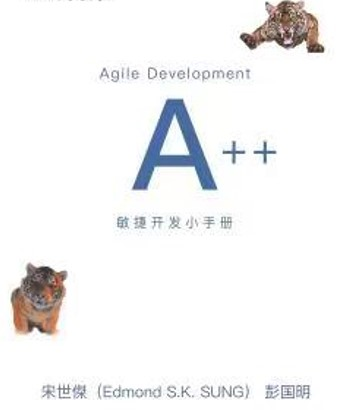
\includegraphics[width=13cm]{aBookCover2latexScreenshot2023-03-08130046.jpg}
\clearpage\newpage \thispagestyle{empty} \mbox{} \cleardoublepage

\thispagestyle{empty} \vspace*{7em}{\centering\Huge A++ 敏捷开发小手册 \par}{\centering -- 从个人提升到 以数据说话 \par}\cleardoublepage

\thispagestyle{empty} \vspace*{\fill} \parbox{.8\textwidth}{\raggedright \scriptsize
\textit{impossible} publisher 2022

printed blindfolded

design: \LaTeX
}
\end{titlepage}
\clearpage \thispagestyle{empty}\cleardoublepage
\newpage % Make sure the following content is on a new page

%----------------------------------------------------------------------------------------
%	TABLE OF CONTENTS
%----------------------------------------------------------------------------------------

\tableofcontents % Prints the table of contents

%----------------------------------------------------------------------------------------
%	INTRODUCTION SECTION
%----------------------------------------------------------------------------------------

%\includeonly(filename,filrname,.......)

%\input(filename)


\chapter*{序} % Introduction chapter suppressed from the table of contents


杨立东 《微管理》作者,四维世景科技(北京)有限公司 总经理

这是一本从事敏捷开发和过程改进的人员的必修之书,作为本书的早期读者,有两个创新让我印象深刻。其一是本书的写法,类似《金刚经》体,全文多是以对话的方式,让读者读起来轻松流畅,少了长篇大论的说教,而是真实和不同IT企业高管、中层、甚至开发团队的问答,在问答中将普遍问题进行归纳总结,并提出解决的方法。其二是案例和数据的引用,虽然很多作者都在书籍中应用案例和大量数据,宋老师则是结合自己多年的从业经验,对案例和数据精益求精,每个案例都颇具经典。通过阅读和理解这些案例,更能体会对话中的问题,以及形成的解决方案的建议。

读过很多管理类的书籍,有些管理数据自始至终贯穿一条主线,例如德鲁克的《卓有成效的管理者》,有些书籍则以故事的形式给企业管理做出启示,例如《目标》。本书的内容始终贯穿过程改进的主题,将宋老师多年在该领域的咨询和培训经验跃然纸上,其中也引用了很多小故事,让书籍活跃了起来,让读者读起来不至于太累。诚然,一千个人有一千个哈姆雷特,具体大家在书籍阅读中去体会吧。

给我感触更深的是宋老师的严谨的写作态度,每次他写完一章,都发给不同的管理者去阅读和提出改进的建议,每次的问题都会得到反馈和在章节中得以应用。这种态度是非常值得尊敬的,毕竟在该领域他才是货真价实的专业人士,而我们这些先期读者只是普通的从业者。

最后,预祝书籍能帮助到那些有志于在管理上提升的从业人员。

\begin{description}
\item[]
\begin{description}
\tightlist
\item[]
2023年3月于北京
\end{description}
\end{description}


\chapter*{感谢 Acknowledgments } % Introduction chapter suppressed from the table of contents

6年前开始把一些培训、评估经验,配合软件工程/项目管理知识,写分享文章,在公司网站和CSDN上发布;2018年在香港教ACP敏捷课也加深了我对敏捷的了解,也发现很多人未了解敏捷开放的重点。初始时候缺乏经验,虽然有些很有趣的题材,但未能组成系列性文章,后面逐步某注销组成系列,分享文章也越来越多被转载。2022年受疫情影响,少出差,可以有更多时间把文章组成书,幸运有各朋友的帮助,终于可以在2023年出版。

非常感谢我的老师、客户、学生和朋友们,如果没有与他们面对面的详细讨论,并在项目过程中反复试验与反馈,不可能写出这本书。这些宝贵经验帮我验证了各种敏捷思路与量化管理的可用性,也让我更加清晰地理解了质量改进的重点。

也感谢朋友圈里各位老师、行业精英们分享经验和意见:其中包括北京的杨立东、王绍军、纪钟涛、武宏伟,天津的韩淑军,上海的周青龙,杭州的胡蕊莉,成都的杨杰等。
感谢杭州的徐洪洋在百忙之中抽空提出了文字上的建议;感谢无锡的陈镜庆、秦瑜不断提出修改意见,并帮助我最后完成本书的编辑;也感谢香港李启良先生对
Mediawiki服务器,Linux,LATEX 等平台的技术支持。%done-1

%\input(xuzhang)

%\chapter*{感谢 Acknowledgments } % Introduction chapter suppressed from the table of contents

6年前开始把一些培训、评估经验,配合软件工程/项目管理知识,写分享文章,在公司网站和CSDN上发布;2018年在香港教ACP敏捷课也加深了我对敏捷的了解,也发现很多人未了解敏捷开放的重点。初始时候缺乏经验,虽然有些很有趣的题材,但未能组成系列性文章,后面逐步某注销组成系列,分享文章也越来越多被转载。2022年受疫情影响,少出差,可以有更多时间把文章组成书,幸运有各朋友的帮助,终于可以在2023年出版。

非常感谢我的老师、客户、学生和朋友们,如果没有与他们面对面的详细讨论,并在项目过程中反复试验与反馈,不可能写出这本书。这些宝贵经验帮我验证了各种敏捷思路与量化管理的可用性,也让我更加清晰地理解了质量改进的重点。

也感谢朋友圈里各位老师、行业精英们分享经验和意见:其中包括北京的杨立东、王绍军、纪钟涛、武宏伟,天津的韩淑军,上海的周青龙,杭州的胡蕊莉,成都的杨杰等。
感谢杭州的徐洪洋在百忙之中抽空提出了文字上的建议;感谢无锡的陈镜庆、秦瑜不断提出修改意见,并帮助我最后完成本书的编辑;也感谢香港李启良先生对
Mediawiki服务器,Linux,LATEX 等平台的技术支持。%done-1

%\input(ganxie)

\chapter*{前言 Prologue} % Introduction chapter suppressed from the table of contents

\begin{quote}
We are uncovering better ways of developing software by doing it and helping others do it.\\
--Agile Software Development Manifesto
\end{quote}

敏捷宣言已经有超过二十年的历史,国内越来越多软件开发团队开始采用敏捷和迭代,但总体效果参差不齐。有些年轻的团队成员听到敏捷不需要文档,以为也不需要注重代码质量,包括代码可读性,导致后面发布的软件产品问题多多,难以维护。要编写出高质量的代码,人本身能力非常关键,但软件工程快速发展,导致编程员人数快速增长,其中很多缺乏专业工程师素养,所有若要敏捷开发真正起作用必须先提升编程员能力。\\
没有数据就无法管理,但很多敏捷团队只是走流程(每天站立会议、看板并非敏捷的重点),缺乏度量,所以管理者一听到敏捷就觉得不靠谱,要求团队用回传统的瀑布开发方式。\\
这二十年来,中外都出版了很多关于敏捷的书,但绝大部分都没有深入去探索以上的问题。这本书就是希望通过解读各种敏捷最佳实践,加上敏捷以外的其他知识,帮助大家理解并更好使用敏捷,提升软件的质量和总生产率,让团队成员与公司管理层获得双赢。\\
同时也希望管理层通过这本书能了解敏捷开发的要素,并能使用敏捷开发模式,帮助公司提升软件产品质量,同时降低成本增加公司的竞争力。\\

\framebox{%
\begin{minipage}[t]{0.97\columnwidth}\raggedright
某技术总监陈总在5天差距分析的最终总结会里问开发团队:

\begin{enumerate}
\tightlist
\item
  你们知道自己是每天产出多少代码行吗?(生产率)
\item
  你们知道平均修复一个系统测试的缺陷花多少工作量(人时)?
\item
  有没有发生过:代码开发完成,系统测试人员尝试运行,但跑不动?(开发人员不能借口说不懂业务,或需求不清,因为你写完代码后,自己连最基本确保代码能运行都没有去做。我还未问你们做开发的有没有做好单元测试/集成测试。)
\item
  你们做测试的知道测试覆盖率是多少?
\end{enumerate}

陈总有丰富开发经验,他最后总结说:
``我以前自己做开发时也是被问过这些问题,我当时也不懂,但我能知耻而后勇------先知道现在的不足,然后按评估老师的最佳实践,持续改进。''\strut
\end{minipage}}

\begin{itemize}
\tightlist
\item
  如果你像陈总下面团队一样,不懂以上问题的答案,这手册可以帮你自己找答案。
\item
  如果你(是管理者或客户/用户)不满意团队的软件开发成果,这手册可以帮你找出根因,启发团队改善。
\item
  如果你已经很了解,恭喜你,但应还可能从这手册里找到一些你未知但有用的方法。
\end{itemize}

\framebox{%
\begin{minipage}[t]{0.97\columnwidth}\raggedright
1980年,STROUSTRUP
先生不满意当时很流行的C语言,因为在70年代,已经有如SmallTalk之类的面向对象语言,C是基于传统步骤式的语言,没有面向对象的功能,所以STROUSTRUP先生就基于C的基础,加上有类功能的C
(C with
Classes)。过了4年,他同事觉得这个名字不好,就改成C++,也出了一本书叫C++,与本来经典的C很相似。后面C++就成为了面向对象的常用语言。\\ A++
继承40年前
C++的思路,希望在敏捷(Agile)开发的基础上,加上增值的元素,更能帮助团队与管理者做好软件开发,让客户满意。\strut
\end{minipage}}
%done-1

%\input(qianyan)

%----------------------------------------------------------------------------------------
%	BOOK PART
%----------------------------------------------------------------------------------------


\chapter{如何改善敏捷开发质量} % Introduction chapter suppressed from the table of contents


\framebox{%
\begin{minipage}[t]{0.97\columnwidth}\raggedright
按瀑布式阶段开发的困难:\\毕业后参加的开发项目,客户是电信行业,很规范,所以有一定的里程碑和阶段要求。有分析阶段、设计阶段、编码阶段,最后交付,里面当然包括一些测试。\\但往往因为客户的需求不断变化,每一两周都会有新的要求,因为电信业面对的市场变化也很大。导致本来我们预计六个月的项目,后面会有三到四周的测试和调试。也因为不断的有需求变化,不断在修改,几乎就没有时间做好测试,导致为了赶本来合同规定的交付时间,后期不准熬夜加班,更惨的是没来得及测试好,很多代码还是有不少缺陷。\\ 其中一个原因,如果可以把本来前面的设计画UML图的时间省略掉,应该可以腾出更好的时间来做后面的开发和测试。所以当张工开始接触敏捷开发,很相信这种快速交付迭代的方式可以对团队有帮助。\strut
\end{minipage}}

\hypertarget{ux67d0ux8f6fux4ef6ux5f00ux53d1ux516cux53f8ux654fux6377ux5f00ux53d1ux8fc7ux7a0bux6539ux8fdbux6848ux4f8b}{%
\subsection{某软件开发公司敏捷开发过程改进案例}\label{ux67d0ux8f6fux4ef6ux5f00ux53d1ux516cux53f8ux654fux6377ux5f00ux53d1ux8fc7ux7a0bux6539ux8fdbux6848ux4f8b}}

\hypertarget{ux6708}{%
\subsubsection{5月}\label{ux6708}}

张工是公司的中层管理,管理好几个开发团队,有五位项目经理向他汇报。\\
他听说老同学的团队都开始用敏捷开发,很感兴趣,并参加了一些敏捷的交流会,觉得可以解决很多传统瀑布性开发的不足,尤其是可以快速交付给客户。\\
他要求部门经理全面推动敏捷开发,对团队成员进行相关培训,例如,SCRUM Master 内部培训。\\
开始时,张工上级部门经理有些怀疑,问:“后面那些工程文档都不做,会不会影响质量和交付?客户都是专门做电信的,不缺钱,但是对质量要求很高。”\\
张工便解释说,“只要利用敏捷把过程变成迭代,快速交付,改善工程的问题不难,主要是人的问题。”\\
部门经理听到敏捷可以比以前更快速交付,之前客户经常因为延误而不满,他希望可以改变这现状,就答应了。 \\

\hypertarget{ux6708-1}{%
\subsubsection{8月}\label{ux6708-1}}

开发组长王工周五下班后与朋友喝酒,开开心心说: “太兴奋了。研发部门经理决定全面推动敏捷开发SCRUM;我们团队刚参加了两天培训,真正对应我们以前的传统瀑布式开发的种种问题,我们会2周一次迭代,快速反馈,我们会定期小步向客户发版,我们会与用户经常交流,获得他们的反馈。\\
现在团队合作不像以前只按工种工作,也会跟产品经理、业务方面更充分合作,给客户带来更高价值。\\
工作方式也改变了,以前要写需求、规格说明书,现在简单化成用户故事和产品需求卡片,以前我们要做过详细项目计划甘特图,现在用改成用燃烧图和白板。每天用便利贴去写要开发什么东西贴在白板上面,开始的时候,贴的越多感觉越敏捷,我们改成叫 SCRUM team,有一系列的海报围绕我们。我们也没项目经理了,自己管理自己。本来的部门经理现在变成产品负责人,敏捷开发方式让我们团队自己做决策,不仅仅是技术方面,项目相关的也由我们项目组一起讨论决定。\\
解除了以前‘瀑布式开发’的种种烦恼,这一切太完美了。“\\

\hypertarget{ux6708-2}{%
\subsubsection{9月}\label{ux6708-2}}

”你们团队学完敏捷SCRUM后,项目如何?”\\
王工充满自豪地说:\\
“我们培训后就SCRUM的方法,定每两周一个冲刺,每次冲刺前都会用故事点来估算每个功能多大,然后按本次冲刺的资源,估计可以完成多少功能?\\
然后用白板来监控模块完成的情况,哪些在开发中,哪些已经完成,团队和管理者都可以一目了然,不用像以前天天问我们了。我们每天早上也按照SCRUM的规定站立会议,每人说自己完成了哪些任务,今天做什么。\\
大家都很兴奋,确实跟以前瀑布的做法不同。”\\

\hypertarget{ux6708-3}{%
\subsubsection{10月}\label{ux6708-3}}

”你们项目如何?”\\
王工听完,想了一下,然后说:\\
“我们本应上周要完成一次冲刺后的割接上线,但被推到下次了。“\\
”为什么?”\\
王工说: ”我们按培训学到的做冲刺计划会,按照产品的待办事项列表,团队利用扑克牌一起估算每一事项所需要的时间。我们总共八位开发人员,其中有一半是刚毕业不久,但大家刚上完培训,很有信心,虽然技术主管张工对我们出来的估算有些顾虑,觉得我们太理想,但大家刚培训完敏捷,张工也希望让部门经理尽快看到敏捷开发可以加快速度,我们就按这‘进取式’估算开展2周冲刺。\\
但因新人多,编码水平有限,虽然大家已经尽快把开发出来的代码交给系统测试人员手工测试,依据测试发现的缺陷修正再测试,但越来越接近答应客户的2周割接上线时间,但是还是很多BUG没改好,最后几天,基本就天天加班,最终到验收时,仍然有不少问题,最终割接前测试,还是不能达到客户要求的水平,没办法,未能上线。\\
大家确实都尽力冲刺了,但未能达到我们本来希望的结果。“ \\

\hypertarget{ux6708-4}{%
\subsubsection{11月}\label{ux6708-4}}

部门经理之前收到客户总监电话,投诉一些技术缺陷,导致好几次不能按计划上线,问为什么正在交付的软件质量变差了?\\

张工被问到是什么原因时无法回答,只能说立马回去探索原因,尽快汇报,但心里想: “开始敏捷后,因为快速迭代,以前要做概要设计、详细设计的过程反而被忽略了,导致有些写出来的代码,后面就很很难适应快速的变化修改,导致要不然就功能做不出来。 因要赶时间,可以按客户的要求时间交付的话,由于本身代码不好,只可以临时凑凑,不长久。”\\
张工从部门经理办公室出来后,找其中一位项目经理李工喝茶,回顾一下发现项目团队对这次敏捷SCRUM的改革有意见。例如上层为了更快速交付,实现敏捷可以快速交付承诺,把一些本来不太可能的进度时间压到团队去,完全不是本来的那种自主团队管理的概念。出现问题多了,就请了敏捷教练过来辅导,但SCRUM的教练也缺乏软件工程的基础,只懂项目管理过程。所以他们也解决不了软件相关的问题。只是把精益管理怎么做迭代,怎么做回顾这些基本过程再解读一下,解决不了实际问题。\\

李工:
”因为我们做这块业务已经很多年了,本来业务的变化不多,只是一些小的功能改动,所以开发人员尽量不去动核心的代码,怕改动了反而会影响投产,切割不了。但有时为了满足一些新功能,继续在老代码的基础上去写,这种做法效率很低,也不长久,估计一两年后会难以运行了,我们会被迫重写整个产品,而老代码开发人员大部分都离开了,后面的代码维护变得非常困难,即使用敏捷也解决不了这个问题。”\\

无论张工或李工也没有能去总结出什么好的解决方案。现在推行敏捷才刚刚三个月,绝不能打退堂鼓,回到本来的状态。但应怎么解决敏捷带来的问题?挽回部门经理与客户的信心呢?\\
\hypertarget{ux5982ux4f55ux6539ux5584}{%
\subsection{如何改善}\label{ux5982ux4f55ux6539ux5584}}

从以上案例看到,本来管理层希望利用敏捷开发,加快软件开发的交付,减少延误,令客户更满意。但因为只注重项目管理,但没注意和改善软件开发本身的质量,人员能力等因素,开发出来的软件缺陷比以往多,导致后面大量返工,恶性循环,后面更导致延误,最终客户投诉。\\
因为软件本身设计有问题,导致软件难以修改,开发人员都不敢改动任何代码,怕可能会引起系统崩溃。\\

怎样可以确保开发出来软件的质量?\\

敏捷开发有很多种方法(SCRUM 只是其一),因为目的不仅仅是管好项目进度,也要确保软件产品的质量。所以SCRUM 只包括项目管理部分,不全面,反过来,例如极限编程(XP eXtreme Programming),因它的发明者Kent BECK 本身是一位精通面向对象的编程员,所以XP不仅仅关注项目管理,也包含编程的最佳实践。下图是 Ron Jeffery 把XP的重点画成从外到内3层: \\

%\href{文件:cleanagile_f1.8.jpg}{500px}。


\includegraphics[width=10cm]{cleanagile_f18.jpg}

SCRUM 只包含了外层的部分,缺乏中间和内层元素。
按XP的12实践(详见附件)都做到了便可以解决张工的问题吗?\\
不一定。

\framebox{%
\begin{minipage}[t]{0.97\columnwidth}\raggedright Dr
Juran,德鲁克(Drucker)和戴明(Deming)博士是同代人,出生日期相差不超过十年,他们3位都在战后去过日本,帮助日本企业家改善他们的质量。\\在50年代,当德鲁克被ASQ记者问为什么他声称Dr
Juran是现代生产管理之父?\\ 德鲁克解释说:\\现在我们常用的精益(Lean)生产和JIT,其实都是源自Joe
(Joseph Juran)
的过程管理思路,他一直主张要从工作过程入手,从产出反过来决定过程应该如何配合。虽然他没有用"精益"这个词,但他很明白要管理好生产,必须以如何使工人能最好发挥为本,但他这思路被美国很多学术界人士和工业工程师反对:``为什么不是应该由管理者做主,生产者反而成为主角?''\\ 其实戴明、Joe和我都很理解从上而下那一套管理方式是行不通的。日本战后急于回复经济,很接受我们的管理思路,并立马执行,例如丰田40年代未开始推JIT,赶上并超越美国的工业生产。比如我一直和通用汽车(GM)有交流,发现他们就不懂必须先梳理好过程这个概念,从产出反推生产过程应如何配合。尽管GM投入数以亿计的资金自动化信息化,希望改善机器及物流管理,但却不知道本应从过程入手,导致生产到今天也无法追上日本(那套JIT的汽车生产模式)。虽然Joe的思路很清晰,也知道怎么改进企业的质量,可惜一直默默耕耘,没有受到该有的重视。\\ 注:ASQ=American
Society of Quality; JIT=Just-In-Time\strut
\end{minipage}}


下面我们回顾质量大师Dr JURAN 的质量策划方式,如何提升产品质量。\\
客户问:你说Juran先生?\\
我:是的。\\
客户:会不会他的那套质量改进方法太老了,不适用于我们现代。而且他主要关注制作业,不太熟悉我们IT业。\\
我:你听过乔布斯吗?\\
客户:当然听过了,他是苹果创始人。\\
我:乔布斯被苹果赶出来后,自己开创NEXT公司,希望创作未来新一代的电脑产品。他很希望产品在质量方面比较出众。当时,他觉得美国很多企业家都忽略了质量,感觉到被日本的竞争对手赶上。乔布斯便邀请了Dr
Juran从美国东岸飞到西岸,帮他的NEXT公司做辅导,改进过程。(关于他对Dr
Juran的评价,详见附件)

%\href{文件:jobs1Screenshot_2022-06-12_082703.jpg}{100px\textbar{}缩略图}

\includegraphics[width=10cm]{jobs1Screenshot_2022-06-12_082703.jpg}

后面乔布斯回到苹果,大部分NEXT工程师也跟着他一起进入苹果。所以我们现在用一些苹果产品,多多少少都会受当时NEXT质量改进的影响。

我:首先要定义质量是什么?\\

\framebox{%
\begin{minipage}[t]{0.97\columnwidth}\raggedright
质量包括两部分:

\begin{description}
\tightlist
\item[]
满足客户需要 (客户包括外部客户和内部客户)

没有缺陷\\
\end{description}

这定义不仅仅适合于制作业、也适用于服务业,IT业。\\
\strut
\end{minipage}}



我:记得您比较懂财务,对吗?\\
客户:是的,其实我对软件开发还是外行,但较了解财务。\\
我:财务管理是不是包括财务策划、财务监控,财务改进?\\
客户:是的\\
我:Dr
Juran就用财务管理比喻质量管理,同样也有质量策划、质量控制和质量改进。你觉得这个大框架再细分要如何制定质量目标,如何来制定度量等。

%\href{文件:finAnalogyScreenshot_2022-10-07_212149.jpg}{文件:finAnalogyScreenshot
%2022-10-07 212149.jpg}

\includegraphics[width=10cm]{finAnalogyScreenshot_2022-10-07_212149.jpg}

从下表可以看得出来。所以如果我们希望利用敏捷开发,不仅仅是走迭代,确保进度没偏差,还要确保软件产品的质量,也应该用Dr
Juran的质量管理框架去看整个敏捷过程,才能更全面了解如何才可以确保软件开发的质量,也控制好交付工期,不延误,让客户满意。\\
质量策划还包括:

\begin{enumerate}
\tightlist
\item
  设定目标,包括外部和内部目标
\item
  识别内部需求
\item
  依据客户需求制定产品的功能特征
\item
  制定产品和过程的目标
\item
  设计过程来达到这些目标,最后验证过程能力\\
\end{enumerate}

可以用下图了解质量控制和质量改进,比如图的左面就是在过程之前的策划部分。如我们发现缺陷比率为20\%,这就是过程的能力,这个能力是策划的时候已经定好的,过程控制没有什么可以做,只是当缺陷有变化,比如特别高的时候,需要做一些措施返回本来的水平。要改进必须用质量改进,比如希望把缺陷百分比从20\%降到3\%,这就必须驱动一系列的改进计划。改进计划必须要按项目推行执行,没有其它办法。\\
%\href{文件:JuranImprovementScreenshot_2022-10-23_211444.jpg}{500px}

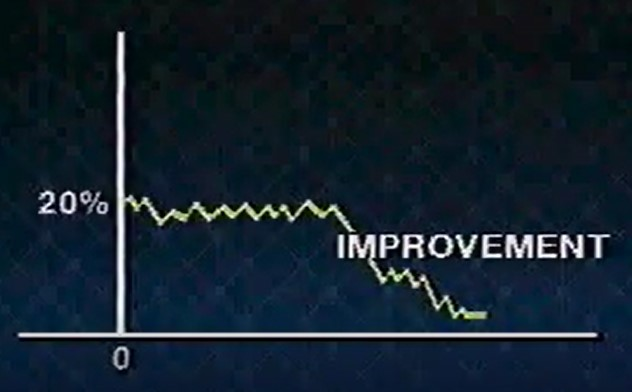
\includegraphics[width=10cm]{JuranImprovementScreenshot_2022-10-23_211444.jpg}

过程改进的计划一般包括:

\begin{enumerate}
\tightlist
\item
  如何识别选择项目。
\item
  组织改进项目的项目团队
\item
  找出缺陷根因
\item
  制定改进措施
\item
  验证是否在真正操作环境里面有效
\item
  处理团队文化上面的抗击阻力
\item
  控制保持本来的水平\\
\end{enumerate}

%\href{文件:IntroXPnJuranStepsScreenshot_2022-10-27_194505.jpg}{550px}

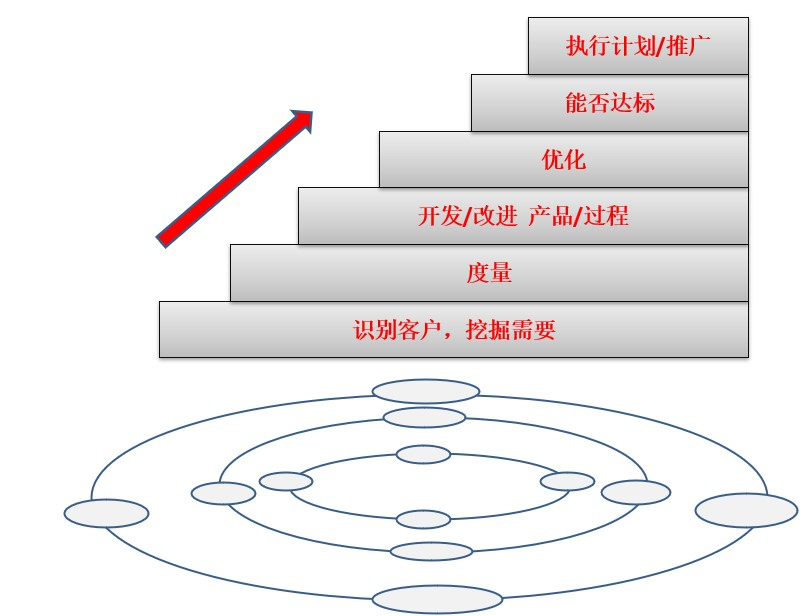
\includegraphics[width=10cm]{IntroXPnJuranStepsScreenshot_2022-10-27_194505.jpg}

客户:你说的策划、控制、改进都挺有道理,但如何跟敏捷,尤其是你说极限编程的实践关联呢?\\
我:任何最佳实践,如果没有定质量目标,配上度量衡量和策划,都只是空想,对长远提升公司文化、团队成员的习惯没有任何帮助。举例:参照上图,例如我们想改善团队的策划和估算。首先要识别客户,哪些是主要干系人
-
甲方有什么要求;内部部门经理,有什么要求。然后从他们的诉求变成过程的功能和特征,但如果特征只是描述,没有数字也没有意义,所以要配合可衡量的度量单位,和用什么方式去收集那些数字,然后依据目标定过程要怎么去做,怎样改。例如

\begin{itemize}
\tightlist
\item
  是否应该从本来的瀑布策划方式制定大的总计划,改用精益的思路,分成迭代,
\item
  每次估算应该怎么做、如何监控等
\item
  然后改进的过程要不断从实验中优化
\item
  最后还要用数字证明这改善比本来好,然后在其他团队全面推广\\
\end{itemize}

而不是单纯`空降'某敏捷流程(例如 SCRUM),便能加快团队的发布速度。
所以虽然极限编程里每一条实践都是最佳实践,也必须配合质量策划,和监控改进才会有效果。

\framebox{%
\begin{minipage}[t]{0.97\columnwidth}\raggedright
很多人都知道戴明环代表PDCA(Plan-Do-Check-Act),其实持续改进的道理也不是戴明博士发明,Juran
对它的了解与应用不会比戴明差。\strut
\end{minipage}}

要注意在整个过程里,高层起非常关键的作用:\\
所以Dr
Juran强调高层不能把公司的质量工作下放(例如,由某助手负责)。我们的经验就是这种做法往往导致最后质量不会有任何改进。原因很简单,每位中层管理者都有一定的KPI标准,资源也是固定的。如果这些没有根本的改变,质量是不会提升,因为整个管理环境没有变化,项目经理、部门经理还是会按以前的做法继续操作,不会听高层的口号或宣传,很快整个质量改进将会失败而终,所有的活动尤其质量相关的,高层必须亲身参与。包括制定质量目标,参与质量提升的高层委员会,定期监督进展等。

这手册会:

\begin{itemize}
\tightlist
\item
  先从个人如何提升,与自我管理开发过程开始
\item
  然后以团队如何做好迭代回顾(复盘)为改进试点\\
\end{itemize}

利用实际案例让大家了解如何开展过程改进。\\
然后,针对每条XP实践,探索如何能在团队里用上,并能改善开发产品的质量(降低客户缺陷密度)。\\
改进都要有衡量才具体,``度量与分析''部分会从基础概念开始,探索如何建立标杆(基线)与预测模型。\\

\hypertarget{ux9644ux4ef6}{%
\section{附件}\label{ux9644ux4ef6}}

\hypertarget{xp}{%
\subsection{XP}\label{xp}}

\hypertarget{ux7f16ux7801ux5b9eux8df5-coding-practices}{%
\subsubsection{编码实践 Coding
Practices}\label{ux7f16ux7801ux5b9eux8df5-coding-practices}}

\hypertarget{cp1ux7b80ux5355ux5730ux7f16ux7801ux548cux8bbeux8ba1-code-and-design-simply}{%
\paragraph{CP1:简单地编码和设计 Code and Design
Simply}\label{cp1ux7b80ux5355ux5730ux7f16ux7801ux548cux8bbeux8ba1-code-and-design-simply}}

\begin{itemize}
\tightlist
\item
  To produce software that is easy to change 使软件易于更改
\end{itemize}

\hypertarget{cp2ux65e0ux60c5ux5730ux91cdux6784-refactor-mercilessly}{%
\paragraph{CP2:无情地重构 Refactor
Mercilessly}\label{cp2ux65e0ux60c5ux5730ux91cdux6784-refactor-mercilessly}}

\begin{itemize}
\tightlist
\item
  To find the code's optimal design 找到代码的最佳设计
\end{itemize}

\hypertarget{cp3ux5236ux5b9aux7f16ux7801ux6807ux51c6-develop-coding-standards}{%
\paragraph{CP3:制定编码标准 Develop Coding
Standards}\label{cp3ux5236ux5b9aux7f16ux7801ux6807ux51c6-develop-coding-standards}}

\begin{itemize}
\tightlist
\item
  To communicate ideas clearly through code 通过代码清晰地传达想法
\end{itemize}

\hypertarget{cp4ux5171ux540cux7684ux8bcdux6c47-develop-a-common-vocabulary}{%
\paragraph{CP4:共同的词汇 Develop a Common
Vocabulary}\label{cp4ux5171ux540cux7684ux8bcdux6c47-develop-a-common-vocabulary}}

\begin{itemize}
\tightlist
\item
  To communicate ideas about code clearly 清楚传达软件设计的想法
\end{itemize}

\hypertarget{ux5f00ux53d1ux5b9eux8df5-develop-practices}{%
\subsubsection{开发实践 Develop
Practices}\label{ux5f00ux53d1ux5b9eux8df5-develop-practices}}

\hypertarget{dp1ux6d4bux8bd5ux9a71ux52a8ux5f00ux53d1tdd-test-driven-development}{%
\paragraph{DP1:测试驱动开发TDD
Test-Driven-Development}\label{dp1ux6d4bux8bd5ux9a71ux52a8ux5f00ux53d1tdd-test-driven-development}}

\begin{itemize}
\tightlist
\item
  To prove that code works as it should 来证明软件正常工作:\\
\end{itemize}

\begin{description}
\tightlist
\item[]
- Test-first programming(prim practice\#)
\end{description}

\hypertarget{dp2ux7ed3ux5bf9ux7f16ux7a0b-pair-programming}{%
\paragraph{DP2:结对编程 Pair
Programming}\label{dp2ux7ed3ux5bf9ux7f16ux7a0b-pair-programming}}

\begin{itemize}
\tightlist
\item
  To spread knowledge, experience and ideas 传播知识、经验和想法:\\
\end{itemize}

\begin{description}
\tightlist
\item[]
- Pair Programming(prim practice\#)
\end{description}

\hypertarget{dp3ux96c6ux4f53ux8d1fux8d23ux5199ux597dux4ee3ux7801vs-ux53eaux987eux8651ux81eaux5df1ux7684ux4ee3ux7801-collective-code-ownership-vs-individual-own-code}{%
\paragraph{DP3:集体负责写好代码(vs 只顾虑自己的代码) Collective Code
Ownership (vs individual own
code)}\label{dp3ux96c6ux4f53ux8d1fux8d23ux5199ux597dux4ee3ux7801vs-ux53eaux987eux8651ux81eaux5df1ux7684ux4ee3ux7801-collective-code-ownership-vs-individual-own-code}}

\begin{itemize}
\tightlist
\item
  To spread the responsibility for the code to the whole team
  将写好代码的责任扩展到整个团队:\\
\end{itemize}

\begin{description}
\tightlist
\item[]
- Whole team(prim practice\#)

- Share code(corollary practice\#)
\end{description}

\hypertarget{dp4ux6301ux7eedux96c6ux6210-integrate-continually}{%
\paragraph{DP4:持续集成 Integrate
Continually}\label{dp4ux6301ux7eedux96c6ux6210-integrate-continually}}

\begin{itemize}
\tightlist
\item
  To reduce the impact of adding new features 降低添加新功能的影响:
\end{itemize}

\begin{description}
\tightlist
\item[]
- Incremental Design(prim practice\#)

- Single code base(corollary practice\#)

- Ten-minute Build(prim practice\#)

- Continuous Integration(prim practice\#)
\end{description}

\hypertarget{ux5546ux52a1ux5b9eux8df5-business-practices}{%
\subsubsection{商务实践 Business
Practices}\label{ux5546ux52a1ux5b9eux8df5-business-practices}}

\hypertarget{bp1ux5c06ux5ba2ux6237ux6dfbux52a0ux8fdbux56e2ux961f-add-a-customer-to-the-team}{%
\paragraph{BP1:将客户添加进团队 Add a Customer to the
Team}\label{bp1ux5c06ux5ba2ux6237ux6dfbux52a0ux8fdbux56e2ux961f-add-a-customer-to-the-team}}

\begin{itemize}
\tightlist
\item
  To address business concerns accurately and directly
  准确、直接地解决业务问题:
\end{itemize}

\begin{description}
\tightlist
\item[]
- Real Customer involvement(corollary practice\#)
\end{description}

\hypertarget{bp2ux8ba1ux5212ux6e38ux620f-play-the-planning-game}{%
\paragraph{BP2:计划游戏 Play the Planning
Game}\label{bp2ux8ba1ux5212ux6e38ux620f-play-the-planning-game}}

\begin{itemize}
\tightlist
\item
  To schedule the most important work 安排最重要的工作:\\
\end{itemize}

\begin{description}
\tightlist
\item[]
- Weekly cycle ; Quarterly cycle ; Slack (prim practice\#)
\end{description}

\hypertarget{bp3ux5b9aux671fux53d1ux5e03-release-regularly}{%
\paragraph{BP3:定期发布 Release
Regularly}\label{bp3ux5b9aux671fux53d1ux5e03-release-regularly}}

\begin{itemize}
\tightlist
\item
  To return the customer's investment often
  尽早交付,让客户看到投资回报:
\end{itemize}

\begin{description}
\tightlist
\item[]
- Incremental Deployment(corollary practice\#)

- Daily Deployment(corollary practice\#)
\end{description}

\hypertarget{bp4ux4ee5ux53efux6301ux4e45ux7684ux901fux5ea6ux5de5ux4f5c-work-at-a-sustainable-pace}{%
\paragraph{BP4:以可持久的速度工作 Work at a Sustainable
Pace}\label{bp4ux4ee5ux53efux6301ux4e45ux7684ux901fux5ea6ux5de5ux4f5c-work-at-a-sustainable-pace}}

\begin{itemize}
\tightlist
\item
  To go home tired, but not exhausted 回家时虽然很累,但不筋疲力尽:\\
\end{itemize}

\begin{description}
\tightlist
\item[]
- Slack (prim practice\#)
\end{description}

\hypertarget{ux4e54ux5e03ux65afux8c08dr.juran}{%
\subsection{乔布斯谈Dr.Juran}\label{ux4e54ux5e03ux65afux8c08dr.juran}}

\framebox{%
\begin{minipage}[t]{0.97\columnwidth}\raggedright
他(NEXT CEO)接受访谈时,对美国企业,质量,和 Dr.Juran
观点的重点内容:\\
美国已经富裕了很多年。很多企业都忘记要获得成功,还是要关注基本功,包括教育。现在我们美国很多企业面临困难,处处感觉被日本领先了。其实不是日本针对我们,而是我们作为美国企业家应反思一下,为什么我们的战略比他们差,为什么我们的策划不如日本?我们知道Dr.Juran
在40/50年代多次去日本,帮助日本企业提升质量。现在他回到美国,希望把他的经验带到美国企业,提升竞争力,可以再一次成为世界第一。

我觉得Dr.Juran
很实在,不是泛泛而谈。我们的工程师也深受他这种风格影响。无论我们之中谁问他问题,总裁还是工程师,他都会全心全意用自己的知识解答。所以工程师和我都很希望用他那套方法来做提升。整个质量提升的道理其实很简单,是一个重复的过程,然后我们需要不断去看,有哪些无效的环节要省略,哪部分要重新设计,不断试验、提升,就这么简单。重点是所有的提升都应该是科学化的,有数据而不是泛泛而谈。

一般管理层的思路是:我是领袖,你们应该听我命令。但应该是反过来,让应如何做好的决定权利放在团队手上,做改进不需要请求管理层的批准。改进是工作的一部分,整个架构扁平化,自己管控日常过程,每位工程师应像以前的工匠,愿意花精力不断做好。然后能以自己最后做出的优质工艺、产物自豪。\strut
\end{minipage}}%done-1

%\part{案例分析}

\part{个人提升}自我改善效率基本功\\

\chapter{克服拖延症} % Introduction chapter suppressed from the table of contents


技术总监问:现在我遇到最大的难题就是如何提升下面技术人员的能力,如果他们全都是高手,我就很轻松了,但实际上高手最多只有三分之一,其他都是中低水平。您接触过这么多软件开发团队,有什么好方案?\\
我:你可以先听听以下故事。\\

\begin{description}
\tightlist
\item[]
= = = = = = = = = =
\end{description}



%\url{文件:超效率目录.png}

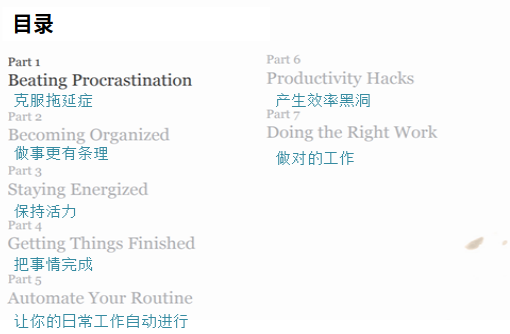
\includegraphics[width=6cm]{Screenshotfrom2023-10-1523-05-00.png}

例如,第一章克服拖延症,这里的内容几乎全部都有帮助:\\



\hypertarget{ux6839ux56e0ux5206ux6790ux8befux89e3ux6848ux4f8b}{%
\subsubsection{周/日目标 (1 Weekly/daily Goals)}\label{ux6839ux56e0ux5206ux6790ux8befux89e3ux6848ux4f8b}}

\framebox{%
\begin{minipage}[t]{0.97\columnwidth}\raggedright
我每天都会定计划,早上希望完成哪些功能,下午完成哪些。当然这个计划也会按实际的进展调整。

周 /
日目标是个人时间管理的基本功。每一天第一件事不是回邮件,而是仔细想想今天要完成什么任务,每一周的开始,也应该想我本周希望完成什么任务。不然的话,每天的时间就很容易被琐碎的小事吃掉,一事无成。\\
\strut
\end{minipage}}

\framebox{%
\begin{minipage}[t]{0.97\columnwidth}\raggedright
背后体现的道理很简单, 要把时间花在重要、但非紧急的活动上,效率才会体现出来。

%\href{文件:紧迫非紧迫_3.0.png}{600px}
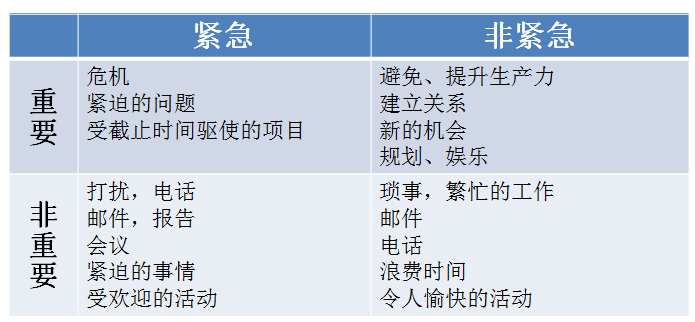
\includegraphics[width=6cm]{紧迫非紧迫30.png}

\strut
\end{minipage}}

\hypertarget{ux6839ux56e0ux5206ux6790ux8befux89e3ux6848ux4f8b}{%
\subsubsection{限定时间 (Timeboxing)}\label{ux6839ux56e0ux5206ux6790ux8befux89e3ux6848ux4f8b}}

\framebox{%
\begin{minipage}[t]{0.97\columnwidth}\raggedright
 把每天的任务安排成时间段,每一段不应超过1.5小时。\\ 
一般人可以专心集中的时间段都不会超过60分钟,小孩可能更短。如果老师叫你星期五5点钟交卷,你不会提前交,都会等到最后十分钟,甚至最后五分钟。所以如果我们把一天的时间切开,分成
1 ~ 1.5 小时时间段,自然有动力,希望在时间之内完成任务。\\
我们写代码的时候应该也是用同样的原理。例如某些编程活动尝试了多次,但没有进展,有时总共会花超过10小时。所以每次当我发现某编程工作超过了2小时,我就会先做其他事情。\strut
\end{minipage}}


\hypertarget{ux6839ux56e0ux5206ux6790ux8befux89e3ux6848ux4f8b}{%
\subsubsection{分解任务 (Dissolving tasks)}\label{ux6839ux56e0ux5206ux6790ux8befux89e3ux6848ux4f8b}}

\framebox{%
\begin{minipage}[t]{0.97\columnwidth}\raggedright
因为都是练习题,所以每一个功能都比较细,不会超过二十行。如果我们平常做开发时,也必须要把一些大、复杂的功能预先拆分成小的功能才有效率。
\strut
\end{minipage}}


\hypertarget{ux6839ux56e0ux5206ux6790ux8befux89e3ux6848ux4f8b}{%
\subsubsection{加强自律 (Building Self-Discipline Muscles)}\label{ux6839ux56e0ux5206ux6790ux8befux89e3ux6848ux4f8b}}


\hypertarget{ux6839ux56e0ux5206ux6790ux8befux89e3ux6848ux4f8b}{%
\subsubsection{晨礼(Morning Rituals) 日常运动 (Make an Exercise Routine)}\label{ux6839ux56e0ux5206ux6790ux8befux89e3ux6848ux4f8b}}


\framebox{%
\begin{minipage}[t]{0.97\columnwidth}\raggedright
不要以为编码是一个单纯的脑力活,整天坐在电脑前面敲代码就可以。如果人的体力、精力没有配合上也会出问题,好在我每天早上一直坚持30
\textasciitilde{}
40分钟的轻量运动,然后晚饭前半个小时到一个小时的骑单车或者慢跑的习惯。中间也是不是整天坐着,一段时间会走一走、喝点儿橙汁等,以确保身体不断在动,这样才不会困,保持动力。

贝多芬每天都会通过去外面散步来获得一些创作的灵感,然后他会立马把这些写在本子上,用于后面的音乐创作。
\strut
\end{minipage}}

我:身体健康,精神状态也同样重要,你每周有锻炼的习惯吗?\\
小李:没有,每天都太忙了,虽然一直觉得身体不如几年前了,也知道锻炼好,但无法抽出时间。\\
我:我也很忙,但深知定期运动对身体非常重要,我一直按以下两方法保持个人身体状态:

\begin{itemize}
\tightlist
\item
  工作时尽量避免长期坐下来,因我主要做培训、咨询、评估,所以可以大部分时间站着或在走动(NEAT\#)。
\item
  尽量每天7点吃早餐前跑圈,疾跑1.5 -
  2分钟,休息半分钟,重复这循环4-6轮(HIIT\#)。
\end{itemize}

\hypertarget{ux6839ux56e0ux5206ux6790ux8befux89e3ux6848ux4f8b}{%
\subsubsection{不会分心的工作场所 (Create a Distraction-Free workplace)}\label{ux6839ux56e0ux5206ux6790ux8befux89e3ux6848ux4f8b}}

\hypertarget{ux6839ux56e0ux5206ux6790ux8befux89e3ux6848ux4f8b}{%
\subsubsection{轻策划、迭代、再策划 (Ready , Fire, Aim!)}\label{ux6839ux56e0ux5206ux6790ux8befux89e3ux6848ux4f8b}}

\framebox{%
\begin{minipage}[t]{0.97\columnwidth}\raggedright
三十年前,软件开发都是一些大型的项目,整个架构要设计好才动手去写代码。现在反过来,需求变化极大,开发都需要敏捷,轻文档、轻计划,尽尽快写好代码,做一些功能给客户,从反馈优化下一轮。我这次的几天开发也是用同样原则,没有花时间在一些设计或者文档。想直接把代码写出来,并通过单元测试,节省了很多耗时间的工作。把有限的时间都放在写好代码上。
\strut
\end{minipage}}


\hypertarget{ux6839ux56e0ux5206ux6790ux8befux89e3ux6848ux4f8b}{%
\subsubsection{不断清洗 (Churning)}\label{ux6839ux56e0ux5206ux6790ux8befux89e3ux6848ux4f8b}}

\framebox{%
\begin{minipage}[t]{0.97\columnwidth}\raggedright
万事开头难。我在开始的半天也是遇到同样问题,不知如何入手,太久没看写代码的书了,很多基本的都不知如何入手。所以我开始的时候不会直接尝试写题目里面的功能,而是重写一些书本的代码,看看跑出来怎么样,然后逐步提升。写一些基本功能,慢慢有了习惯,调整过来了,后面就越来越顺。好比一台旧的水泵,刚开始抽上来的水总是有难喝的铁锈,只要不停止抽水,当污水最终都从系统中抽出后,就能发现底下的净水。
\strut
\end{minipage}}

\hypertarget{ux6839ux56e0ux5206ux6790ux8befux89e3ux6848ux4f8b}{%
\subsubsection{要有好的土壤 (Remove your Hidden Roadblocks)}\label{ux6839ux56e0ux5206ux6790ux8befux89e3ux6848ux4f8b}}

\framebox{%
\begin{minipage}[t]{0.97\columnwidth}\raggedright
在含盐量高的土壤里种植物是结不出果实的。浇水、平衡在阴凉处和阳光下的时间都抵不过根部吸入的毒素。如果我们没有积极性,就可能是土壤的问题。如果没有足够的积极动力,就不会在长假专注写程序,也不会定期要求自己写分享文章。所以要有明确、很想达到的目标驱动。
像一个作曲家,他希望写出很多经典的优秀作品,不满足于现在的状态。觉得自己的灵感或者创造力没有发挥出来,成为可以保留下来的东西。也是这种驱动力让我可以一直努力做这件事。
\strut
\end{minipage}}


\hypertarget{ux6839ux56e0ux5206ux6790ux8befux89e3ux6848ux4f8b}{%
\subsubsection{摒弃拖延恶习 (Quit your Procrastination Vices)}\label{ux6839ux56e0ux5206ux6790ux8befux89e3ux6848ux4f8b}}

\framebox{%
\begin{minipage}[t]{0.97\columnwidth}\raggedright
长假里,大部分人都会把时间用于看视频或电视剧,而我正好没有这个习惯,也一直没有玩网络游戏的习惯,否则肯定完成不了。
\strut
\end{minipage}}

最终我用日程记录(Timelogging),把整件事和什么活动、时间花在什么地方都记录下来了。

小李:我看你上面列出的技巧,我大部分都还没做到。

我:不要紧,我六年前刚开始定期写文章时跟你一样,但只要不放弃,一直往既定目标努力,不良习惯都改正过来了。我常常说人的潜力是极大的。舒伯特你听过吗?\\
小李:好像是一个很有名的作曲家。\\
我:是的,但他31岁就去世了,你猜他一生一共写了多少首歌和音乐作品。\\
小李:我记得中学时,老师介绍过他的艺术作品,如《鳟鱼》,但他31岁就死了,我猜100 \textasciitilde{} 200 首歌?\\
我:他一生写了超过460首歌曲(时长\textgreater{}24小时)。除了歌曲,他还写了其他作品,如9首交响曲(1首未完成,1首只有草稿),20
室内乐,120 钢琴曲等,每一类都包括大量经典作品,对后世影响深远。\\
小李:如果粗算一下,他一生约有600作品,算他有16年时间作曲,平均每月要完成3个作品,真是不得了。\\
我:虽然他的作品有大有小(从一首歌到45分钟的交响曲),他确实生产率极高,而且他最后的7年身体一直都不好,所以他那个时候肯定不会像我们现代996方式工作。
他每天主要是早上用来写作,傍晚便去休息散步。但他会同时做多个创作项目。
如果项目没有灵感,就暂时放下来,创作其他作品。
他著名的未完成交响曲就是个好例子,只有两个乐章(一般交响曲都是四个乐章)
所以他是使用高效技巧的一个成功例子。
每个人都有自己的理想,但如果没有高效率来执行,理想只是天马行空,天方夜谭,不会有任何成就。
除了以上这些技巧外,保持整洁也重要。你有没有试过想找某东西,找半天都找不着?

小李:确实经常发生,而且还会遗漏东西。我上次出差便忘记了iPhone,后面回北京后电话联系当地酒店前台后,我找当地同事去酒店取,然后快递给我,烦死了。\\
我:有听过5S (5S法\#)
吗?例如,如果你把东西都放固定地方,就可以避免同类问题再发生。如果你一直在一个很乱的环境工作,回导致心情烦躁,对工作、身体都不好。

\begin{description}
\item[]
\begin{description}
\tightlist
\item[]
(\#详见附件”锻炼之道”的多了解  NEAT, HIIT;5S法详见第1章附件。)
\end{description}
\end{description}

小李:我大概懂你的意思了,要提升自我能力先要改变习惯,有了良好习惯(如时间管理),才可能提升。\\

\begin{description}
\tightlist
\item[]
= = = = = = = =
\end{description}

总监:我大概懂你的意思了,要提升技术人员的能力先要改变他们的习惯,有良好的习惯(如时间管理),才有机会提升。\\

\framebox{%
\begin{minipage}[t]{0.97\columnwidth}\raggedright
即时笔记 (The Capture Device)
总监边听边在本子上记下那些重点。高效的人都会有工具帮他记录想到的灵感、想法、项目、待做事项等,不会仅仅靠大脑记忆。你提出一个要求,他会立马写在小本子上,你会觉得他应该会按你要求去处理,但反过来如他只是口头说会处理,你会担心很可能没有下文。但我看有些领导,身边只拿个手机,除非他们的记忆力超人,否则我估计他每天都会忘记不少重要事项。
\strut
\end{minipage}}

\hypertarget{ux7ed3ux675fux8bed}{%
\subsection{结束语}\label{ux7ed3ux675fux8bed}}

\framebox{%
\begin{minipage}[t]{0.97\columnwidth}\raggedright
杭州某高级经理的高见
人一定要自律!您说的小技巧确实能起到很大帮助,而且我基本都会使用,但如果不养成习惯,想起来使用下,最终还是改不了拖延症,所以要解决拖延症,一定从根源做起,还是得靠自己,需要培养自己意志力、专注力,坚持好习惯,改掉坏毛病。
\strut
\end{minipage}}

我相信人分高低,但并非取决于基因、种族,主要取决于她后天的习惯、自律与努力。要养成良好习惯要从小开始,深受家庭和教育的影响,所以百年树人。

与公司改进一样,改变个人习惯很难,这些技巧可以帮助个人改善。

\hypertarget{ux9644ux4ef6}{%
\section{附件}\label{ux9644ux4ef6}}


\hypertarget{ux953bux70bcux4e4bux9053-the-truth-about-exercise}{%
\subsection{锻炼之道 The Truth about
EXERCISE}\label{ux953bux70bcux4e4bux9053-the-truth-about-exercise}}

想大家都同意和相信:
``多运动,便多烧耗卡路里,便能帮助减肥,降低体重。''

\framebox{%
\begin{minipage}[t]{0.97\columnwidth}\raggedright
某国家给市民的健康指南:每周起码做150分钟中强度锻炼,或75分钟高强度锻炼。
\strut
\end{minipage}}


但不是每个人都能每天抽时间做锻炼,有什么更好方法?\\
不一定只依赖去健身室锻炼,平常工作生活少坐多走,站着工作、开会,甚至小动作等都有帮助。

\framebox{%
\begin{minipage}[t]{0.97\columnwidth}\raggedright
N.E.A.T. (Non-exercise activity thermogenesis) 小实验;
教授使用有电子传感器的底裤,记录记者、咖啡厅女服务员、商务人员三人一周每天正常工作中消耗多少卡路里。\\
发现:

\begin{itemize}
\tightlist
\item
  女服务员最好。因每天都非常忙碌(尤其是早餐时段),送餐、接单、做咖啡等等。
\item
  商务人员第二。虽然有很多时间坐下来,但每天都会走一公里路见客户,而且每周二、五下班后会去健身锻炼。
\item
  记者最差。每天无论工作或家里,大部分时间都是坐下不动,所以他看起来不胖,但其实体内存有大量脂肪,集中在肝、肾等内脏。
\end{itemize}\strut
\end{minipage}}

这实验告诉我们:如果每天一直坐下不动很不好,就算每天下班后晚上都去健身锻炼也帮不了。

后面记者听教授建议,改变习惯,定期站起来走动。如与同事交流与尽量边走路边交流,减少长期坐下来;
多爬楼梯,少用电梯;骑单车,不开车等方式。
后面,从实验数据分析,发现这些改变帮他增加每天卡路里消耗接近一倍,到500水平。

研究发现不断大量健身锻炼不一定对每个人都有效。
有20\%会没有效果,另一端对15\%的人会非常有效。
这跟人的基因密切相关,所以多锻炼不一定都有效。

\begin{description}
\tightlist
\item[]
= = = = = = = = =
\end{description}

实验发现,如锻炼能快速提升心跳率到最高,然后休息,反复做 4 - 6轮,
效果不会比大量健身锻炼差。
例如,每天做几轮40秒的冲刺,把心跳速度快速提升到极限,
效果可以比长时间的缓步长跑更好。

\framebox{%
\begin{minipage}[t]{0.97\columnwidth}\raggedright
HIIT (High Intensity Interval Training) 小实验;
教授与助手教记者使用运动单车做 HIIT:
用尽全力练20秒,休息,再同样做两轮;每周三次。

记者按教授要求完成了四周HIIT锻炼,虽然帮他提高了血液分解糖份的能力,减少糖尿病风险;
但提升不了他的最高带氧运动量。教授解释这是因记者的遗传基因是属于没有效果的20\%。
\strut
\end{minipage}}

\hypertarget{ux53c2ux8003-references}{%
\section{参考 References}\label{ux53c2ux8003-references}}

1. YOUNG, Scott: "The Little book of Productivity" 《超效率手册》\\


%1011

\part{自我管理开发过程}软件开发工程师自我改进过程\\


\part{利用评估开始过程改进}团队必须先获得管理层的关注与支持\\

\part{从做好迭代回顾开始 }因为项目变数很多,不应传统地制定详细长期计划,然后按这计划执行、监控,而应该按照精益概念,把项目分成多轮迭代( 2 – 4 周),每迭代开发部分功能,并每轮与客户确认能否满足客户需求,避免把精力浪费在一些没有价值的工作。 如果想改进,每次迭代后的回顾是最好时机:团队分析本迭代数据,识别有那些不足,找出根本原因,制定可在下轮迭代执行的纠正措施。\\

这部分讲述应如何做好迭代回顾,分4章讨论迭代回顾的:\\

1.成功基础要素\\
2.根因分析的主要部分\\
3.详细步骤与常见问题\\
4.最后怎样可以从定性提升到定量(利用数据预测模型)\\



\chapter{根因分析} % Introduction chapter suppressed from the table of contents

\hypertarget{ux5206ux6790ux4e8bux6545ux6839ux56e0ux4e0aux96c6}{%
\subsection{分析事故根因:上集}\label{ux5206ux6790ux4e8bux6545ux6839ux56e0ux4e0aux96c6}}

北京的某软件开发公司,专门为电信供应商做定制软件开发与运营,比如用短信做些推广活动等。公司希望做过程改进。\\
我:
过程改进的主要目的是帮助企业更好地达成业务目标。你们应该是最清楚自己有哪些不足的,请问你觉得哪些方面有改进空间?\\
总经理:
我不太熟悉技术细节,只能从客户视角来看。例如,去年因为软件的一个错误导致客户损失了几十万元,我立即在公司内部开会,希望找出根因,最后发现是因为某个开发人员粗心大意,在编码时把两行数字搞错了,在测试人员针对这项功能进行测试时,虽然收到短信了,但并没有仔细看短信的内容,也就没有发现这个缺陷,测试通过了。这起事故不仅招致了公司的经济损失,更影响了客户对我司的信任度,也影响公司在行业内的口碑。\\
我: 公司采取了哪些纠正措施?\\
总经理:
之后我们加强了对代码的评审工作,要求这类代码都需要经过主管审查,还增加了相应的惩罚措施,
如果再次发生同类事件,项目经理和部门负责人都要承担连带责任。\\
我:采取这个措施之后,效果如何?\\
总经理:很好,大家都注意了,到现在都还没有再发生同类的问题。

\begin{description}
\item[]
\begin{description}
\tightlist
\item[]
= = =
\end{description}
\end{description}

你认为以上的纠正措施能避免同类问题的再次发生吗?\\
你可能赞同以上事故的主因是人员疏忽,但很多事故的主因其实不仅仅是人员疏忽。

\hypertarget{ux9999ux6e2fux5357ux4e2bux6d77ux96be}{%
\subsection{香港南丫海难}\label{ux9999ux6e2fux5357ux4e2bux6d77ux96be}}

\framebox{%
\begin{minipage}[t]{0.97\columnwidth}\raggedright
2012年10月1日晚上8时,任职港九小轮的黎细明驾驶海泰号(注)由中环出发前往南丫岛榕树湾。15分钟后,任职港灯的周志伟驾驶南丫四号从榕树湾出发,接载港灯员工及亲友到维港观赏国庆烟花。两船于8时20分相撞,南丫四号船尾迅速沉没,造成39人遇难。

(注:海泰号是大型喷射双体船,速度与载客量都远比南丫四号高。)

\strut
\end{minipage}}

南丫四号船尾沉没,消防处安排潜水员紧急救援:\\
%\href{文件:LammaAccidentScreenshot_2023-06-01_194248.jpg}{550px}

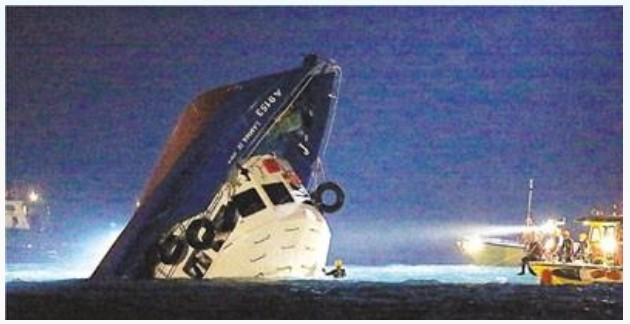
\includegraphics[width=6cm]{LammaAccidentScreenshot_2023-06-01_194248.jpg}

黎细明(左,56岁),小二文化程度,1982年任职小轮公司,2008年成为船长。\\
%\href{文件:CaptainScreenshot_2023-06-01_195518.jpg}{200px}

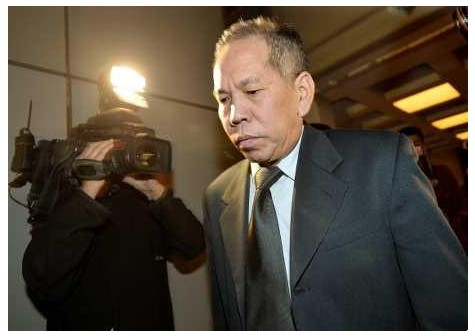
\includegraphics[width=6cm]{CaptainScreenshot_2023-06-01_195518.jpg}

%\href{文件:Captain2Screenshot_2023-06-01_195805.jpg}{150px}\\

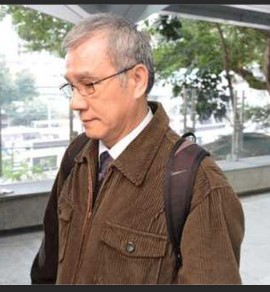
\includegraphics[width=6cm]{Captain2Screenshot_2023-06-01_195805.jpg}

周志伟(58岁),小六文化程度,已婚,育有两女,1974成为海员,1993年开始担任船长。

\framebox{%
\begin{minipage}[t]{0.97\columnwidth}\raggedright
2015年,开庭审判两船长:\\
周:碰撞发生前,南丫四号曾右3转度避撞,但海泰号违规左转3度,且海泰号船速较快及操控性较高,故南丫四号的避撞措施均被海泰号的相反举动抵消。

黎:造成大量乘客死亡的原因是南丫四号船身有问题,包括部分船舱并非水密舱等,而且海上的雾灯及其他背景灯光也影响了我的视线,难以观察到南丫四号。

专家:海泰号没有根据"国际海上避碰规则"右转,反而左转3度,属"极度危险",南丫四号虽曾按规则向右转,但"幅度太小、转得太迟"。

\begin{itemize}
\tightlist
\item
  陪审团以7比2 裁定黎细明误杀罪成立,法官判入狱8年
\item
  陪审团以8比1 裁定周志伟误杀罪不成立,但危害他人在海上安全罪以7比2
  裁定罪成,法官判入狱6个月
\end{itemize}
\strut
\end{minipage}}


你赞同两位船长的失职是本次海难的根因吗?

政府经过3年多的事件调查,最终做出调查报告。报告显示,在海难中沉没的南丫四号,从设计到验收,每个环节都存在纰漏,每个环节都有出错,例如包括:

\begin{itemize}
\tightlist
\item
  没有安装水密门 (导致南丫四号在碰撞另一艘船之后,迅速沉没)
\item
  座位的螺丝松动
  (导致撞船后,因船尾沉没水中,所有座位都松脱,跌到船尾,影响乘客逃生)
\item
  没有儿童救生衣等
\end{itemize}

因此导致南丫四号在碰撞海泰号之后,迅速沉没,并且导致罹难人数众多,政府展开内部调查,怀疑海事处有十七名职员应负责任。

除了南丫四号的问题,你是否觉得小轮公司也应负责任,例如:

\begin{itemize}
\tightlist
\item
  对船长的培训/监督是否足够
\item
  是否有定期检查船上救生设备
\end{itemize}

你可能要反驳,像``南丫四号''这类小型船,预算少,所以关注度、监控度都低,如果是大型项目应该不会出现这类纰漏事故,请看看美国NASA的太空穿梭机(Space
Shuttle)计划因发生了两次致命的事故,最终被叫停的案例。

\framebox{%
\begin{minipage}[t]{0.97\columnwidth}\raggedright
太空穿梭机灾难 (Space Shuttle disasters) \\
1986:挑战者号(Challenger),挑战者号航天飞机升空后,于发射后的第73秒爆炸,机上7名宇航员全部罹难。(
相关视频可以在网上搜到)\\
2003: 哥伦比亚号
(Columbia)航天飞机在返回地球时,因为左翼的隔热保护胶在十六天前升空时被固体火箭助推器外层脱落的乳胶击破损坏,导致航天飞机返航时进入大气层的第1000秒钟,在35,000米高空因过热解体,7名宇航员全部罹难。\\
Sally RIDE 在2003哥伦比亚号灾难事故调查回顾说
:我很诧异这两次事故的原因非常相似 (她也是挑战者号事故调查组员),86
年引起挑战者灾难的陋习又再出现 :
为了赶上计划升空日期,而忽略了之前性能报告的发现,没有注意前线技术工程人员提出的安全隐患,也缺乏安全保障措施。其实从哥伦比亚号在1981年首次升空开始,每次都有出现升空时燃料缸外的保护乳胶掉落的事故,但管理层一直都没有关注,工程师因为赶进度,每次升空前,都没有时间预先处理好。

%\href{文件:2_Space-Shuttle-Columbia-team.jpg}{250px\textbar{}有框\textbar{}左\textbar{}图3:
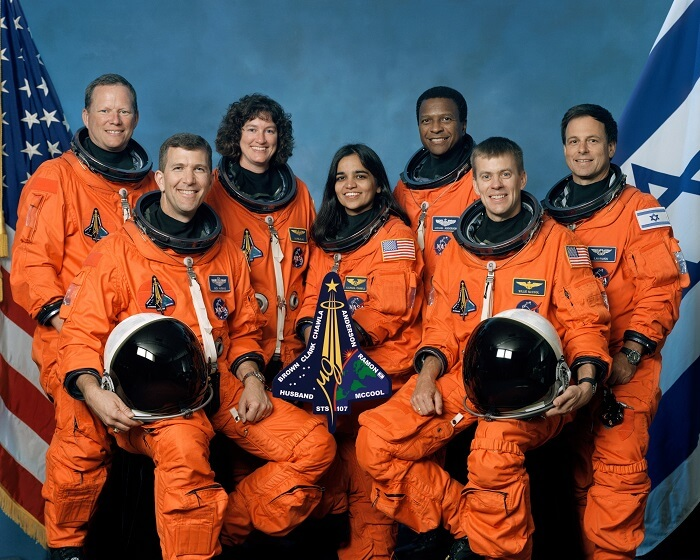
\includegraphics[width=6cm]{2_Space-Shuttle-Columbia-team.jpg}
%7名哥伦比亚号宇航员}\\
\strut
\end{minipage}}

如果管理层、工程师只关注项目的成本与进度,忽略了质量与安全,便会导致灾难。

其它很多相似的航空或海上灾难,虽然当事人(如船长)的失误引发了事故,但这并非根因,背后系统的不足才是主因。

上面总经理的纠正措施能避免同类问题再次出现吗?\\
不一定。因为已经导致公司极大的损失,而且引发了高管的关注,开始的时候大家会注意,但并不能长久,因为这仅仅依赖于个人的习惯,很可能在几个月后还会再次发生。

\hypertarget{ux6839ux56e0ux5206ux6790ux7684ux4e3bux8981ux5143ux7d20}{%
\subsection{根因分析的主要元素}\label{ux6839ux56e0ux5206ux6790ux7684ux4e3bux8981ux5143ux7d20}}

如果想挖掘系统的不足,便必须找出根因,根因分析主要包含那些元素?可参考CMMI模型的根因分析(Causal
Analysis \& Resolution CAR):

%\href{文件:CMMIHM_02.png}{文件:CMMIHM 02.png}

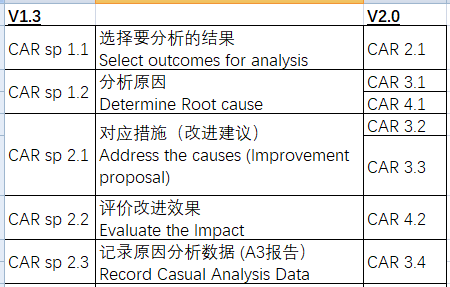
\includegraphics[width=6cm]{CMMIHM_02.png}

\begin{enumerate}
\tightlist
\item
  利用二八原则识别引起大部分问题的最主要因素
\item
  分析背后的主要原因
\item
  对应改进措施
\item
  判断改进效果
\item
  总结成根因分析报告
\end{enumerate}

可参考附录A:
"绅士俱乐部过程改进"了解QC圈如何按意识根因分析元素完成为期七个月的过程改进。本章附件也有二八原则与帕累托图的介绍。但不要误以为只要使用各种根因分析方法,如帕累托图、鱼骨图等,就能做好根因分析.

\hypertarget{ux6839ux56e0ux5206ux6790ux8befux89e3ux6848ux4f8b}{%
\subsubsection{根因分析误解案例}\label{ux6839ux56e0ux5206ux6790ux8befux89e3ux6848ux4f8b}}

\framebox{%
\begin{minipage}[t]{0.97\columnwidth}\raggedright
某公司过程改进组(共4人)分析以往一年项目,做根因分析,希望改进交付的质量,减少交付验收时的缺陷数。

%\href{文件:Epg-car3.1-1.png}{400px}\\
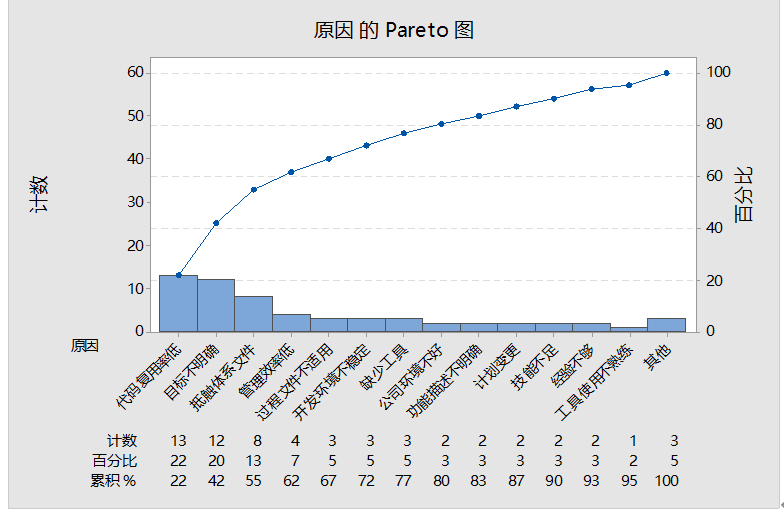
\includegraphics[width=6cm]{Epg-car31-1.png}

\strut
\end{minipage}}

我:请问这帕累托图的依据?\\
组长:针对客户缺陷密度较高的现状,我们做了敏感度分析。发现需求引入的缺陷数跟它相关性最高,我们接下来就用鱼骨图分析,四个人一起头脑风暴,识别出以下十几项主要的原因种类,然后我们就按每人三票,各自单独投票得出这个排序,然后我们就依据二八原则选择了头三项原因是主要的对象,然后我们根据这三项原因发现,这些项目是导致需求缺陷的原因,包括流程图画不好等。

我听完以上根因分析故事,便在投影仪投出以下某机场某年导致航班延误的原因统计表,问项目经理:``假如你是顾问团队,要为机场管理层高层分析导致航班延误的主因并提出改进方案你会怎么利用二八原则画帕里托图?''

\begin{description}
\item[]
\begin{description}
\tightlist
\item[]
香港启德国际机场1996年航班延误统计:
\end{description}
\end{description}

%\href{文件:CRairportDelayScreenshot_2023-06-02_191306.jpg}{600px}
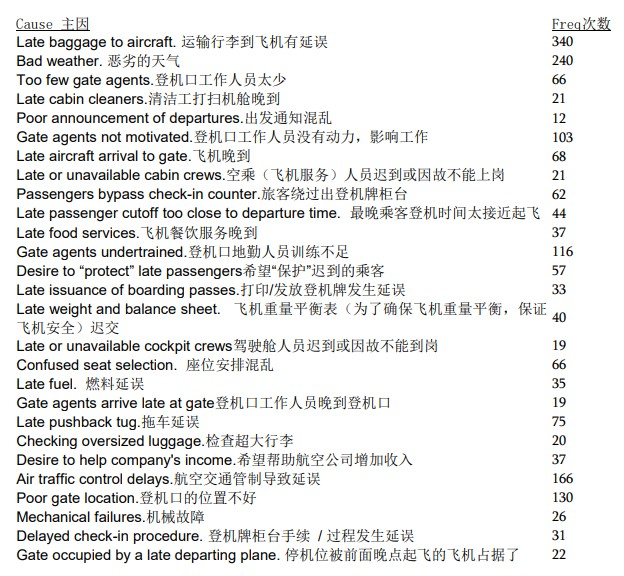
\includegraphics[width=6cm]{CRairportDelayScreenshot_2023-06-02_191306.jpg}


然后我解释:\\
我们不应直接把几十条原因,按每条原因对问题的影响度,从最高排到最低做帕累托图,而应先把原因进行分类。用上面机场延误为例,比如,哪些是不可抗力的天然原因(如天气原因),哪些是跟闸口管理相关的问题,那些是跟机场打印登机牌相关等,例如,如果识别出是跟闸口管理类的问题最多,后面便针对这进一步分析根因。分组才有针对性、有意义。

你们的分类,帕累托图依据的``数据'',都只是用数字形式表达你们头脑风暴的主观判断,
所以你用这种帕累托图其实跟直接用头脑风暴做出做出的结论没什么差异,只是你们用了投票数据使结果看起来``量化''了,其实是没有客观数据支撑。

例如,你们的分类有问题:
例如,只有``功能描述不明确'',难道``非功能需求描述不明确''(如性能、安全性等)就不需要考虑吗?\\
你们现在的分类有不少是重复的,同样一个问题有可能归属于两个、三个分类。

你们度量操作定义有问题,例如,你是如何根据历史项目的数据去判断哪些原因归属于``功能描述不明确''?

如果想做好,应该预先按你们想要解决的问题,识别出相关的度量项,然后针对这些度量项,例如,缺陷,定义如何分类(详见附件``二八原则与数据分类'')并收集数据后,做分析。有了客观的数据分析,才是你们根因分析的第一步。

\begin{description}
\item[]
\begin{description}
\tightlist
\item[]
= = =
\end{description}
\end{description}

我:你们现在的找出的其实并非根因,只是浮在水面上的现象,你们有听过5W吗?\\
组长:有, What When ..\\
我:不,你说的是5W+1H
,5W是五个为什么(why),所以你们应一直追问,才能更好地识别出背后的主因,并针对主因采取纠正措施,才能避免同类问题重复发生。\\
我继续向他们讲述丰田汽车大野耐一先生的5W故事。(详见附件``大野耐一先生5Why例子'')

除了通过问``为什么''之外,模型(例如 CMMI, XP
极限编程等)也可以帮你们更全面地找出根因。
很多原因会导致项目延误。``功能描述不明确''可能只是其中一个原因,例如:

\begin{itemize}
\tightlist
\item
  利用检查单做好需求评审
\item
  与干系人(客户)确认需求
\end{itemize}

如果能做好这些,即可帮助团队确保需求质量,减少项目延误,以上两条都是
CMMI 里的最佳实践,所以模 型可以帮助团队更全面地看问题。

\hypertarget{ux600eux6837ux624dux80fdux505aux597dux6839ux56e0ux5206ux6790}{%
\subsubsection{怎样才能做好根因分析}\label{ux600eux6837ux624dux80fdux505aux597dux6839ux56e0ux5206ux6790}}

从前面各例子看到,有些团队没有根因分析的意识 :
不理解核心思路,只是表面``做''了根因分析的步骤,其实未找到根因。所以,要做好便必须利用培训,提高大家的根因意识。大家从以下日本回国技术总监的故事可以更好理解什么是``根因意识''。

\hypertarget{ux6280ux672fux603bux76d1ux7ecfux9a8cux4e4bux8c08}{%
\subsection{技术总监经验之谈}\label{ux6280ux672fux603bux76d1ux7ecfux9a8cux4e4bux8c08}}

\framebox{%
\begin{minipage}[t]{0.97\columnwidth}\raggedright
总监之前一直在日本带领开发团队,十年前回大陆。最近为他们做过程差距分析,总监开车送我去机场时分享他的日本经历。\tabularnewline
\strut
\end{minipage}}

你说我们团队没有找出真正根因,我非常赞同。日本人在根因分析方面做得特别好。我之前在日本工作,带领小组做开发,当时我们团队共5人,有2位来自大陆,其他是本地人,有一次,因为我们开发计算公积金出错,QA一直追问问题的原因。当时我还没有找出根因的概念,不明白QA的意图,以为只是问责,希望找个人背锅。其实他们确实是希望找出问题的源头,避免同类问题再发生。当时主管追问原因,要求我发问题报告。我的报告只说了一些开发问题,人员经验不足等。主管一直追问为什么。``如果你说培训不足,你有什么相关的培训计划来避免?''我回答不上来。最后发现,原来是日本计算方法和大陆不同,他们不四舍五入,导致我们两位大陆开发人员的计算便和本地的不同。
很多大陆工程师没有根因分析概念,认为质量依靠个人保证,``我负责,有问题我承担''。日本人不是这个思路,他们希望挖掘到问题的根本原因并避免。后面我回国发展,开始时兼职做咨询工作,帮一位老朋友看看某软件开发公司团队的问题,发现很多大陆团队对质量方面的要求远远不如日本,很不习惯。

\framebox{%
\begin{minipage}[t]{0.97\columnwidth}\raggedright
日本产品质量\\
98年,我在香港富士通工作,试图在香港市场推富士通的服务器,富士通服务器跟美国太阳(SUN)匹配(compatible),但价位反比美国太阳服务器高,一直想不出什么原因。后来我去东京出差,发现原来日本公司,例如富士通,对质量特别有要求,产品测试设计等都要通过很多关卡,才可以出厂。有些富士通在澳大利亚的工程师就不明白为什么总公司要求这么苛刻,需要不断测试,觉得浪费资源。他们不清楚原来日本本土客户对质量要求特别高,无论是消费品或电子产品,如果达不到高水平质量要求,基本上卖不出去。富士通公司电子产品以满足本土市场为主,所以必须有很高的质量要求。

客户(甲方)是否对质量有高要求也是促进产品质量的重要因素。\strut
\end{minipage}}

所以如果公司高层没有产品质量的要求,单靠团队学习根因分析技巧不会有改进效果。

\hypertarget{ux7ed3ux675fux8bed}{%
\subsection{结束语}\label{ux7ed3ux675fux8bed}}

根因分析包括下图各主要元素:

%\href{文件:微信截图_20230707090950.png}{600px\textbar{}无}

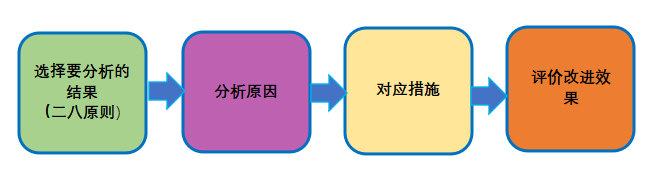
\includegraphics[width=6cm]{微信截图_20230707090950.png}

从上面案例,大家看到如能用好根因分析,应可帮助团队避免同类问题重复发生,帮团队提升。

但要真正做好根因分析不能单靠学理论与方法,必须利用实际数据让团队成员动脑筋和讨论,才能真正用好根因分析,取得效果。

下一章,我们探索针对软件开发如何利用根因分析做好过程改进。

\hypertarget{ux9644ux4ef6}{%
\section{附件}\label{ux9644ux4ef6}}

\hypertarget{ux4e8cux516bux539fux5219ux4e0eux6570ux636eux5206ux7c7b}{%
\subsection{二八原则与数据分类}\label{ux4e8cux516bux539fux5219ux4e0eux6570ux636eux5206ux7c7b}}

帕里托(Pareto)
,16世纪意大利威尼斯人,他发现虽然威尼斯很富有,但财富并非平均分布,80\%财富在20\%手里,他也发现很多其他分布都非平均。

%\href{文件:ToolsParetoScreenshot_2023-06-02_191628.jpg}{400px}

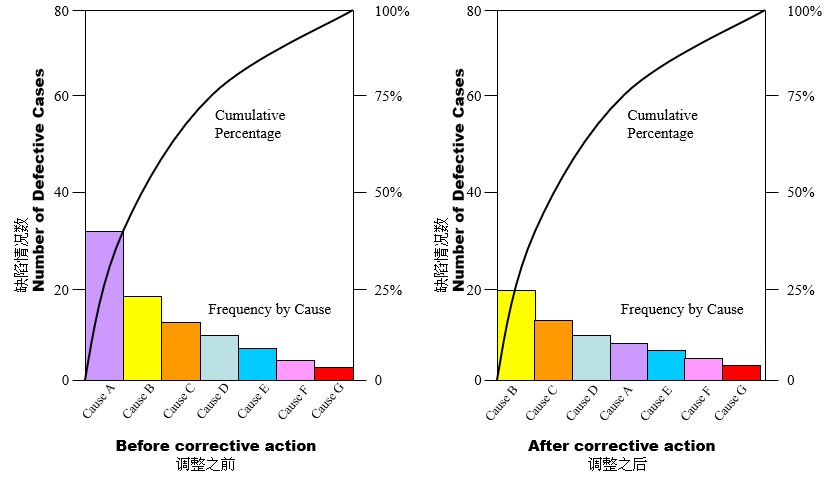
\includegraphics[width=6cm]{ToolsParetoScreenshot_2023-06-02_191628.jpg}

因为过程改进需要公司额外的资源投入,必须有针对性地找出最容易取得改进效果的原因,才可能拥有最大的成功机会。所以,应该利用二八原则去识别影响最大的几个因素.
以上图为例,原本A类问题出现最多,针对这类问题做过程改进之后, A
类问题就少了很多,下一轮便应针对最多的B类问题做改进。

有些人以为,只需要对某个维度做分析即可,并没有从多个维度进行分析

例如,某纸制产品工厂会计数据显示,八成的产品问题相关成本都归属于5类,例如:质量不合格、赔偿、售后现场服务等(共有20类)。
针对5类中最大的一类质量不合格,
发现里面八成的成本都由于六个产品引起(共有50个产品)
针对这六个产品把成本按缺陷种类细分,发现B产品断裂缺陷的成本最高,
我们就应该针对这一问题研究如何改善。

%\href{文件:Ar2_缺陷类型造成的损失.jpg}{文件:Ar2 缺陷类型造成的损失.jpg}

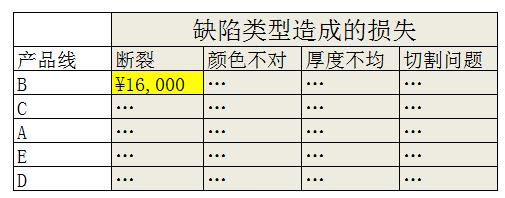
\includegraphics[width=6cm]{Ar2_缺陷类型造成的损失.jpg}

\hypertarget{ux5927ux91ceux8010ux4e00ux5148ux751f-5-why-ux5b9eux4f8b}{%
\subsection{大野耐一先生`` 5 Why
''实例}\label{ux5927ux91ceux8010ux4e00ux5148ux751f-5-why-ux5b9eux4f8b}}

有一次,大野耐一先生见到生产线上的机器总是停转,虽然修过多次但仍不见好转,便上前询问现场的工作人员。\\
(1-Why)问:``为什么机器停了?'' 答:``因为超过了负荷,保险丝就断了。''\\
(2-Why)问:``为什么超负荷呢?'' 答:``因为轴承的润滑不够。''\\
(3-Why)问:``为什么润滑不够?'' 答: ``因为润滑泵吸不上油来。''\\
(4-Why)问:``为什么吸不上油来?''答: ``因为油泵轴磨损、松动了。''\\
(5-Why)问: ``为什么磨损了呢?'' 答:
``因为机器打磨金属零件,空气混进了铁屑等杂质,并掉进机器油缸里。''\\
经过连续五次不停地问``为什么'',找到问题的真正原因(润滑油里面混进了杂质)和真正的解决方案(安装过滤器)。由现象推其本质,因此找到永久性解决问题的方案,这就是5
Why。



%1011
\chapter{如何降低软件开发质量成本} % Introduction chapter suppressed from the table of contents

软件开发不同于工业生产,因都是人的行为,依赖团队成员自己收集。(工业生产依赖自动化机器,容易得到数据。)

\hypertarget{ux6570ux636eux6536ux96c6}{%
\subsection{数据收集}\label{ux6570ux636eux6536ux96c6}}

``如何才能收集到开发质量相关数据,来分析根因,制定纠正改进措施?
因为没有度量,便无法谈改进。''这是很多研发经理想解决的问题。\\
收集软件开发数据有各种困难,如果没有收集到可信的数据,便无从分析与改进。\\
是否可以依赖加强组织级度量与监控?
我们先看看一家过万人,主要提供金融软件产品,公司遇到的困难,公司一直都很强调量化管理,收集各种项目的系数、度量并分析。\\

\hypertarget{ux81eaux52a8ux5316ux7edfux8ba1ux5206ux6790}{%
\subsection{自动化统计分析}\label{ux81eaux52a8ux5316ux7edfux8ba1ux5206ux6790}}

质量部经理:我们每次都跑全量,公司引入低码平台,更多的是在需求设计阶段做好质量保证,
所以我们很注重量化质量管理,能否通过自动化来统计分析,
如何通过量化或工具方式实现自动评审。

我:为什么要自动化?

经理:从去年开始我们搞度量分析, 发现员工就会造数据, 结果导致失真,
度量哪里就造哪里,
所以还是想通过工具代替人工方式,除了能提升效率,也能帮助判断数据是否合理。\\
现在我们的主管很反感度量,一度量就有人造数据。

我:度量本来是件好事。 经理:是的,就是大家知道算法原理就开始造假。
因为我们搞了红黑榜,
但很多人头脑都很聪明,会想办法,但用于不合适的地方。

我们有很多数据统计分析,比如看测试用例与需求的比例。
其实客户发现的缺陷比例也降低了,但因为我们这行对质量特别注重,产品经过多年的逐步演化,过程很复杂,导致软件缺陷的修复很耗时,客户不太满意。
而且公司要求交付的频率要比以前高了很多,我们团队做这些分析都忙不过来,所以需要员工设自动化工具等加快速度才可以。\\
让我给你看看我们大数据分析。

我:等等,但我们首要解决如何能收集到真正的数据,不然数据分析没有意义。

经理:好的,有什么建议?

我:还记得我们上次交流,要让团队自主,不能单靠标准过程并用指标监控执行情况。

%\href{文件:Diagram_2.0.png}{500px}

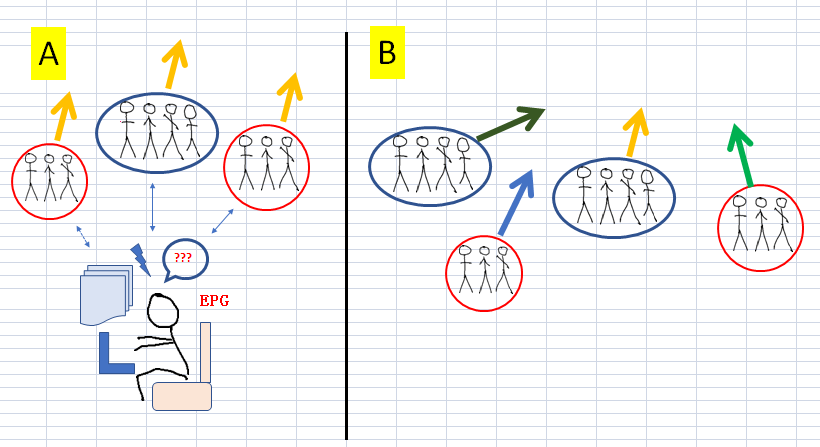
\includegraphics[width=6cm]{Diagram_20.png}

我:请问你们是采用左面还是右面的方法做过程改进?\\
经理:好像我们现在度量分析是采用你图里左面的方法。

我:是的。总体分析还有另一不足:各个项目特性不一样,你们现在几十个项目总体趋势分析,
很可能找不对根因,因每个项目的问题(根本原因)很可能不同。
比如,同样是一个测试用例比例数,你的范围就很宽,从最低的0.3到最高的超过200。但你们取平均值5.1
来做分析。

收集数据也是问题,因为收集数据是挺花精力的工作。

经理:完全同意。

我:但正因为不同项目有各种特性,要对收集到的数据做分析也很耗时。
这些辛辛苦苦做出来的分析报告其实不仅仅是给高层(或者项目经理),
使每一个团队成员都看到才有意义
。(度量分析要反馈回数据提供者,他们才有动力继续收集数据)要把那些分析好的报告再跟每一个团队成员解释要花多大精力?

\textbf{度量的主要目的是从数据分析找出根因做改进而不是仅仅为了监控}

%\href{文件:Ma4CarScreenshot_2021-12-27_205004.png}{400px}

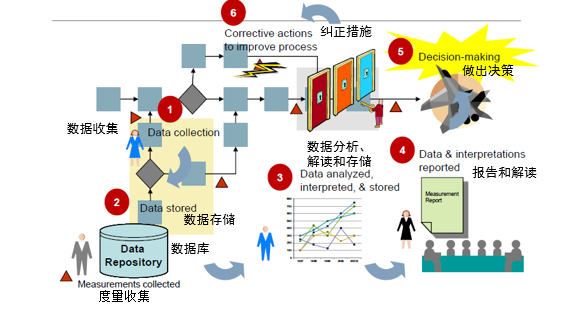
\includegraphics[width=6cm]{Ma4CarScreenshot_2021-12-27_205004.png}

如果把数据分析下放到团队自己搞,便灵活多了;也正因为他们有参与收集和分析讨论,
你们也可以节省很多沟通的成本。

所以你们领导应该定位自己是内部老师,辅导团队怎么做好数据分析,效果会更好。

经理:团队自己讨论便可以得到改进吗?不需要我们领导?\\
我:
如果团队有能力,就应该放手让他们自己收集数据、利用数据进行分析并做出改进。你们应把自己重新定位为团队的教练,去辅导他们如何收集与分析数据。千万不要以为这项工作会比以前自己做分析更轻松,其实你们需要更熟悉整个过程,才能真正辅导好团队。但因为你们之前积累了经验,所以辅导团队应该不会太难。更大的挑战反而是要让管理层了解并赞同,敏捷开发需要团队自主的思路。

\hypertarget{ux6570ux636eux6536ux96c6ux9891ux7387}{%
\subsection{数据收集频率}\label{ux6570ux636eux6536ux96c6ux9891ux7387}}

几个月后,质量经理问:请问老师有没有写过关于客户满意度与产品研发/质量/过程改进之间的关系的文章?我想从研发改进或质量改进的角度,正向推导出如何帮助提升客户满意度的方法。

\begin{description}
\tightlist
\item[]
(公司一直很注重每年的客户满意度调查,高层也会参考满意度调查结果,作为
KPI系数之 一,确定绩效,并决策公司资源的投放等。)\\
\end{description}

我:我没有写过你说的这类分析文章,但有写过客户的案例分享:某香港公司,他们在广州有开发中心专门为香港的客户做软件维护工作,他们的项目采用
SCRUM
敏捷开发,每两周一个冲刺,他们每次做完迭代后,都会要求客户填写满意度调查表,然后做数据分析。(这分享文章的部分内容,详见附录B:``分析迭代客户满意度调查数据'')\\
经理:我刚才看了你发的案例分享,挺好的,但我想要的不是通过分析每一次迭代的客户满意度,让团队做过程改进,我想更宏观一些。每年,我们公司有独立部门做客户满意度调查,已经持续了十年,高层会根据调查的结果判断是否继续向事业部投放资源,也会影响到员工绩效等等,所以其他部门都很关注。但后面越来越发现那些数据的作用不大,因为各事业部都清楚,客户满意度调查的分数很重要,高层也关注,所以都会在调查之前拜访客户,做好准备,确保结果不会太差。\\
我:你们做了这么多年,应该最清楚自己的问题所在,你觉得现在的做法有什么不足?\\
经理:我们的客户满意度调查是每年随机抽样一些客户来做,因为是抽样,又是在每年年底才做,有些时候可能项目在上半年的四五月已经结束了。到年底时,客户对很多几个月前的情况都忘记了。\\
我:是的,为什么不在项目发布后立马就做?\\
经理:这项工作是由独立部门去做,因工作量比较大,每年都是独立策划安排的。其实我们也有在项目发布后就做的调查,不过时间跨度没有年度这么宽。只是一些简单的高中低打分,由一线人员直接去做。\\
我:为什么不能安排你们的客户满意度调查也是在项目的结束时间去开展,这样不就更及时吗?\\
经理:主要是他们的人力有限,资源有限。\\
我:这个不太说得通,我没有说你们每次发布后都要做调查,这会增加工作量,但你们还是可以随机抽样调查,这样及时性就好多了,不会等到几个月后才调查。你们为什么只在每年年底做调查并更新标杆?\\
经理:还有另一个原因,高管很注意客户满意度调查的结果,以此来判断部门的绩效和对事业部的资源投放,所以调查需要与公司年底的预算同步。\\
我:标杆(基线)的更新不应每年只更新一次,而是实时变化的,如果有显著的变化就更新。还有一个问题,你刚才说因为客户满意度调查的结果会被公司高管用来判断部门的绩效和对事业部的资源投放,所以业务部门肯定会非常关注,并想尽办法得到好的结果,比如预先拜访等等。其实这个不但污染了数据本身的准确性,也影响了数据的可信度,让数据变得不客观。\\
经理:好的,我会根据你的意见,在明天讨论如何改革客户满意度调查时,提出建议。\\


\hypertarget{ux54eaux91ccux6700ux8017ux5de5ux4f5cux91cf}{%
\subsection{哪里最耗工作量}\label{ux54eaux91ccux6700ux8017ux5de5ux4f5cux91cf}}

软件开发特点,超过95\%的成本都是人力成本。按二八原则,应先识别最耗工作量的地方?

首先利用二八原则识别出哪类问题的影响最大。在软件开发中,如想提升团队生产率(降低工作量),应先探索哪类工作最耗费工时。

\framebox{%
\begin{minipage}[t]{0.97\columnwidth}\raggedright
\textbf{请你把过去一年的软件开发项目,按不同工种占项目总工作量的比例,从最多到最少排个序?}

\begin{enumerate}
\tightlist
\item
  编码与代码设计
\item
  交付后的所有工作,包括维护、更新与缺陷修正
\item
  交付前的评审,静态扫描,测试与缺陷修正
\item
  项目管理与监控
\end{enumerate}\strut
\end{minipage}}

可以参考本章附件中的“开发项目工作量(成本)分布”,看你的选择与典型分布相差多远。

软件开发项目最大的工作量通常是花在找出与修正缺陷上(开发里的`测试与评审',详见本章附件),
根据软件开发度量专家卡铂斯·琼斯 (Capers JONES)
先生在2012年的研究,对于超过10,000功能点、计划使用25年的大型系统,有接近一半的工作量是与找出并修正缺陷相关。

很多项目中的缺陷大部分还是到后期才发现,这导致了大量返工。如果能提前发现并解决这些缺陷,就可以大大降低研发成本(不仅仅是提升产品质量):\\
::(绝大部分公司都类似:发现缺陷最多的是在系统测试阶段,验收测试阶段其次)\\
%\url{文件:AR1缺陷数.jpg}


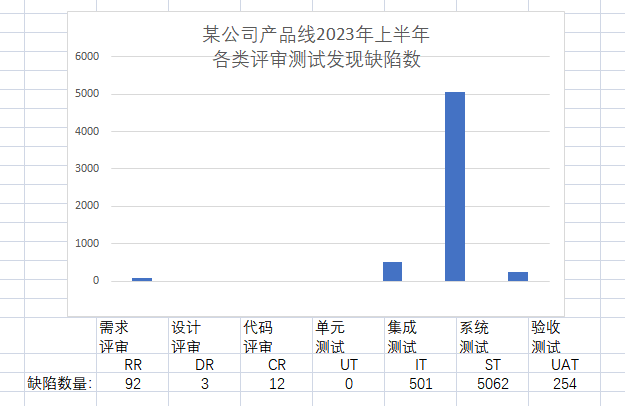
\includegraphics[width=6cm]{微信截图_20231023085822.png}

%由于测试与缺陷修复而造成返工的总工作量,在整个开发项目中占比很高\\

但很多开发人员误以为编码是项目主要工作,忽视了大量因质量问题引起返工,所以只有当管理层了解了尽早发现并排除缺陷是很好的改进方向,并引起重视,公司才有机会改进。

\framebox{%
\begin{minipage}[t]{0.97\columnwidth}\raggedright
有些偏业务的领导可能会质疑,客户不一定关注缺陷密度,只要达到可接受的水平就可以了。

我解释“在软件开发中,减少后期测试才发现的缺陷,不仅仅能提升产品质量,更重要的是能降低研发的总工作量,所以最终能帮助公司省钱。”(详见附件“公司高层不一定关注质量”)
\strut
\end{minipage}}

\hypertarget{ux5206ux6790ux7f3aux9677ux6392ux9664ux7387ux964dux4f4eux8d28ux91cfux6210ux672c}{%
\subsection{分析缺陷排除率降低质量成本}\label{ux5206ux6790ux7f3aux9677ux6392ux9664ux7387ux964dux4f4eux8d28ux91cfux6210ux672c}}

%\href{文件:jalote_emm_7.1_1.0.png}{500px}

\includegraphics[width=6cm]{jalote_emm_71_10.png}

Figure7.1,从需求到设计、编码、单元测试、系统测试、验收,整个开发过程大家都很熟悉(缺陷只会源自需求、设计、编码);需求、设计、编码后都会评审/测试来排除缺陷,但仅仅做评审/测试不一定能确保质量。因为最终验收缺陷数取决于每个步骤能否有效排除当前的缺陷。

所以可以用缺陷排除率(Defect Removal Efficiency DRE)
来衡量测试或评审的效率:

%\href{文件:Ma3_1.0.png}{文件:Ma3 1.0.png}

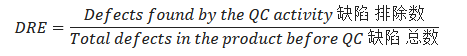
\includegraphics[width=6cm]{Ma3_10.png}

缺陷排除率除了可以用于整个项目,包括测试,也可以用于前面评审、扫描等。

有些人会认为尽早发现并解决缺陷对质量肯定好,但会耗费工作量,增加项目成本,老板不一定愿意。
其实如能在前面预先发现并修正缺陷,便能减小后面测试和修改缺陷的工作量,最终只会减少总项目工作量。

%\href{文件:AR1FixVarCostScreenshot_2022-12-10_144400.jpg}{600px}

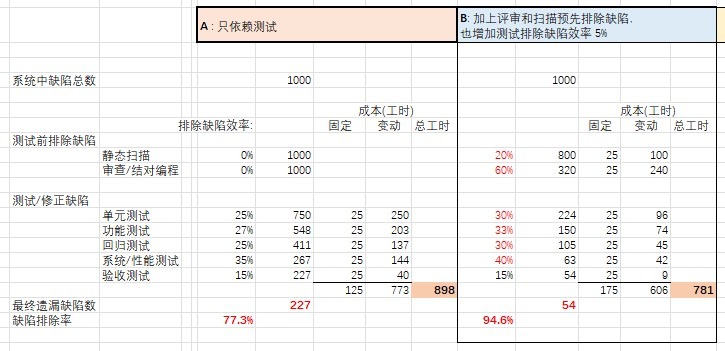
\includegraphics[width=6cm]{AR1FixVarCostScreenshot_2022-12-10_144400.jpg}

比较以上两种策略的质量成本(COQ)就能看出:

\begin{itemize}
\tightlist
\item
  增加测试前扫描与审查,并加大测试效率,不仅减少最终缺陷数到54(对比227),也降低总质量成本(总人时)
\end{itemize}

\framebox{%
\begin{minipage}[t]{0.97\columnwidth}\raggedright
假设:每项任务的固定成本都是25人时;测试前的缺陷修复:每缺陷用
0.5人时;测试缺陷修复,上面计算假定每缺陷用1人时,详见下表:

%Screenshotfrom2023-10-1023-21-23.png
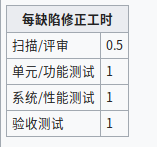
\includegraphics[width=6cm]{Screenshotfrom2023-10-1023-21-23.png}

:*
通常测试里的缺陷修复每缺陷不只1人时,例如在验收阶段时可能要用20人时;我通常会打开这XLS
表,填上客户的估计值。从上表看到,即使用最少的1人时来算,还是不亏。\strut
\end{minipage}}


因为缺陷已经提前被排除系统测试的缺陷减少,测试阶段的工作量减少大于前面扫描评审上的投入。

可以进一步利用COQ概念,增加早期预防缺陷措施,如用原型与客户交流,做好需求调研,进一步减少缺陷和成本。
例如使用原型/场景与客户挖掘需求,可进一步把缺陷降到43,也降低总质量成本:

%\href{文件:est缺陷表3.jpg}{600px}

\includegraphics[width=6cm]{est缺陷表3.jpg}

\texttt{注:你可能会质疑使用原型方法不只25人时,但即使加大到100人时,还是不亏。因它能预防缺陷,使整体缺陷数下降20\%,使总质量成本下降超过100人时。}

正如质量大师裘兰博士 (Dr JURAN) 强调,过程改进应从认同必须改善质量(Proof
of the
Need)开始。如果大家都觉得现在的缺陷水平(例如系统测试超过200个缺陷)是常态,任何公司级质量改进计划都不会有好结果。\\
如果管理层了解现在未能尽早发现并排除缺陷是最好的改进方向(80/20原则)并开始重视,应如何开始?\\
``应先考虑如何能收集到修复缺陷相关工时数据?因没有度量,便无法谈改进。一般团队(如果用系统管理缺陷)只有缺陷统计数据,缺少缺陷返工工作量,测试工作量数据。''
没有缺陷返工工作量数据,开发团队便不会觉得需要前面预先发现缺陷并解决,会以为应让测试人员找出问题,开发人员才修正。
这措施适合于敏捷迭代项目,后面会探索如何在迭代回顾做好数据收集。(但如果用传统瀑布式开发,确实难以解决以上度量难题。过程改进周期会是迭代的好几倍。)\\

\hypertarget{ux7ed3ux675fux8bed}{%
\subsection{结束语}\label{ux7ed3ux675fux8bed}}

可以让团队迭代回顾时收集并分析数据,解决公司级统一收集数据的困难。除了收集开发数据,也需要收集客户反馈数据,才全面,但也应每轮交付收集,才能及时分析数据。缺陷返工占软件开发工作量最多,缺陷越后发现,返工量越大。可以分析缺陷排除率,加强前面的代码扫描与评审,单元测试等,尽早发现并解决缺陷,不仅仅提供产品质量,也降低质量成本,提升团队生产率。

\begin{itemize}
\tightlist
\item
  为了确保质量应该用精益的概念。每一小步确认限制级,确保达标。然后与客户确认,而不是先定一个总体的几个月计划。按总计划监控任务是否延误?因为后者会把团队的关注点都放到按时交付去,无法确保最终的产品达到高质量要求。
\item
  迭代回顾让团队可以每走一小步,回顾有那些不足,分析根因,下一步做改善。如果要从``救火''的管理思路变成基于根本原因找出预防措施的思路,就需要管理者`放手',让团队自己收集数据,自己分析与制定纠正措施。
\item
  收集数据很重要:

  \begin{itemize}
  \tightlist
  \item
    收集数据应与迭代冲刺同步,除了收集团队内数据,也要收集客户的意见,才能全面看清问题
  \item
    如果把数据关连到绩效,很可能会`污染'数据,影响数据的正确性
  \item
    数据有显著变化时,便应更新基线,不要等到年底才更新
  \end{itemize}
\end{itemize}

下一章,我们探索如何策划好迭代回顾与相关培训,让团队回顾后能提升质量和生产率。

\hypertarget{ux9644ux4ef6}{%
\section{附件}\label{ux9644ux4ef6}}

\hypertarget{ux8d28ux91cfux6210ux672c-coq-cost-of-quality}{%
\subsection{质量成本 COQ (Cost of
Quality)}\label{ux8d28ux91cfux6210ux672c-coq-cost-of-quality}}

质量成本由三部分组成:

\begin{enumerate}
\tightlist
\item
  失效(Failure)成本\\
  把缺陷修复好的成本,包括在客户现场被发现的缺陷。
\item
  评测(Appraisal)成本\\
  包括各类测试,如系统测试,集成测试,单元测试等,所花的工时
\item
  预防(Prevention)成本\\
  包括技术评审 (注:有些人把评审归为评测成本,这里按 Mr.Juran
  定义,归属于预防成本)
\end{enumerate}

如变通理解以上COQ定义,``如何通过提高评审效率来降低质量成本``便可对应COQ各部分:\\
失效(Failure)成本:原本所有与缺陷相关的成本\\
评测(Appraisal)成本:增加测试前的静态扫描、评审,减少失效(Failure)成本,使总COQ下降\\
预防(Prevention)成本:减小缺陷的产生,例如用原型做好需求,进一步使总COQ下降\\

\hypertarget{ux516cux53f8ux9ad8ux5c42ux4e0dux4e00ux5b9aux5173ux6ce8ux8d28ux91cf}{%
\subsection{公司高层不一定关注质量}\label{ux516cux53f8ux9ad8ux5c42ux4e0dux4e00ux5b9aux5173ux6ce8ux8d28ux91cf}}

\framebox{%
\begin{minipage}[t]{0.97\columnwidth}\raggedright
{问}:在传统 IT的
公司,无论是 缺陷(Bug)
率还是其他质量指标对业务的影响的相关性都不容易度量,只有重大事件才会让公司在客户面前失去信任,所以高层不会真正的重视质量。\\
{答}:理解,但软件BUG的暴露越往后,返工的工作量就越高,而且是几何级数的增加(例如在单元测试或评审发现都可以1人时内解决;系统测试通常要花起码20人时,客户使用后才发现便更高)。但在很多IT公司,大部分缺陷都是在系统测试、甚至到验收测试才发现。如果能把软件缺陷的发现前移,把通过系统测试、验收测试发现的缺陷减半,便可以大量降低质量成本,提升开发生产率。所以我建议利用缺陷数估算返工的工作量来引起老板重视。(而不是仅仅说降低缺陷率)\\
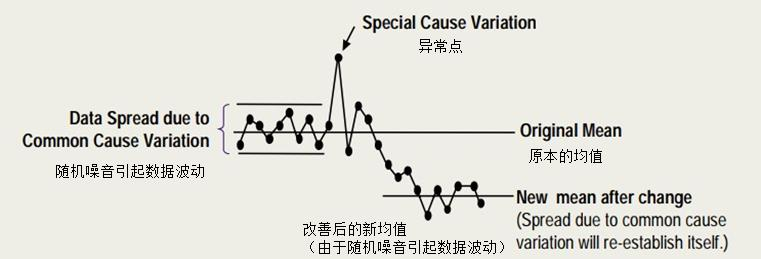
\includegraphics[width=6cm]{MGR_f11.jpg}
\strut
\end{minipage}}

\hypertarget{ux5f00ux53d1ux9879ux76eeux5de5ux4f5cux91cfux6210ux672cux5206ux5e03}{%
\subsection{开发项目工作量(成本)分布}\label{ux5f00ux53d1ux9879ux76eeux5de5ux4f5cux91cfux6210ux672cux5206ux5e03}}

参考Capers JONES先生 2012 的例子,汇总成以下比例:

%\url{文件:AR1成本占比.jpg}
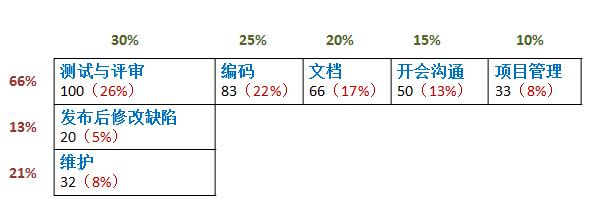
\includegraphics[width=6cm]{AR1成本占比.jpg}

测试与评审一般占开发工作量的30\%,测试与评审一般占总质量成本(包括发布后维护与改缺陷工作)的66\%,把所有工作量都加起来,测试与评审还是占最大(26\%)
, 编码第二 (22\%)。

\framebox{%
\begin{minipage}[t]{0.97\columnwidth}\raggedright
注意:测试与评审包括所有与缺陷相关的成本,包括单元测试、静态扫描、评审与相关的缺陷修正,
而编码只包括设计与编写代码部分。 例如有些人会觉得比例应该是
开发30\%,测试和bug修改25\%,需求和设计20\%,项目管理和沟通20\%,文档5\%。

但如果按上面的定义,开发部分很可能已包括单元测试、静态扫描与改正缺陷工作,
如把这些都归到测试评审里会变回类似上图的比例。\strut
\end{minipage}}


%1011
\chapter{如何做好准备} % Introduction chapter suppressed from the table of contents

\hypertarget{ux5206ux6790ux4e8bux6545ux6839ux56e0ux4e0bux96c6}{%
\subsection{分析事故根因:下集}\label{ux5206ux6790ux4e8bux6545ux6839ux56e0ux4e0bux96c6}}

我:陈总,听说你3年前开始锻炼马拉松,所以现在身体这么好,有什么心得可以让我学习一下?\\
总经理:本来我很胖,也常常很困,体检指标不太理想,我听说可以用长跑锻炼身体,便开始尝试。开始的时候并不容易,因为一直都没有锻炼,先跑五六公里,按程序逐步提升,后面便慢慢养成习惯。最终经过三年锻炼完成马拉松,身体也觉得比以前好多了。\\
我:开始的时候,请问您怎么去持续维持,因为很多人还是一时冲动去锻炼,但持久不了,例如买了跑步机,但一两次后面就没再用了,您有什么心得?\\
总经理:现在支持长跑运动员的度量挺多,最简单的指标就是一公里要多少分钟。我就一直都有度量这个系数来监控进展。比如我开始的时候一公里要接近8分钟,跟走路差不多,后面慢慢就变成7分钟、6分半、6分钟......是锻炼出来的,所以有了这个数,我就知道自己现在是什么水平,是否在进步。\\
我:好比每天跑步锻炼,如果没有手表帮你度量时间速度,你是不知道是否有进步;数据可以给做事的人反馈,让当事人知道差距有多少,所以如果可以从定性提升到定量管理,也可以产生同样的作用。例如评审发现缺陷数量太少,团队应该担心,因为很可能有不少缺陷未被发现,后面到了客户使用时才暴露,代价更大。感兴趣吗?\\
总经理:很感兴趣。\\
我:首先须要利用以往项目数据,建立标杆(基线)例如下图:

%\href{文件:微信截图_20230605130227.png}{500px\textbar{}无}

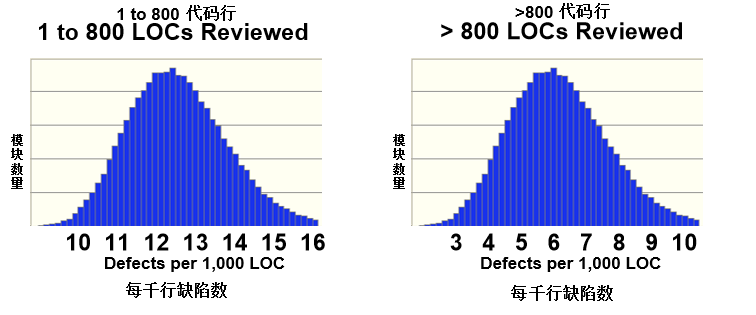
\includegraphics[width=6cm]{微信截图_20230605130227.png}

如果代码是800行以下,每千行代码的缺陷密度均值与范围。800行以上的缺陷密度会低一些,因分母较大。\\
如果某次代码评审,700行的模块,代码评审发现的2个缺陷,比基线下限7个缺陷(注)低很多,团队便应担心,很可能存在不少缺陷未暴露。\\
总经理:但我希望团队有提升,不仅仅是维持,团队怎样可以利用度量数据帮助提升?\\
我:可以利用水晶球模拟,利用缺陷排除率,预估如使用新方法后的缺陷范围。\\
如果也收集团队的缺陷返工工作量,我们更可以预估能降低多少返工。
从降低后面缺陷返工入手,能提高产品开发质量,也能提高团队的生产效率,降低开放成本\\
注:从基线左图,如按每千行代码有10个缺陷为下限,700行代码便应发现起码7个缺陷

\framebox{%
\begin{minipage}[t]{0.97\columnwidth}\raggedright
我用实例在白板上估算提前发现解决缺陷能降低研发成本接近一半。\strut
\end{minipage}}

总经理:很好,应怎么样开始?\\
我:你们有没有团队已经是按迭代开发? \\
总经理:有的,我们去年开始已经有些团队按一个月一个迭代交付,有些更短可能2到3周。\\
我:你们这些团队人员的能力主动性如何?\\
总经理:我觉得还是挺不错的。\\
我:如果你可以识别出2到3个正在在迭代开发的团队,就可以开始做量化的回顾,你们那些迭代团队以前有每轮迭代后做回顾的习惯吗?\\
总经理:都没有。\\
我:首先就要让他们了解什么是根因分析?为什么要做回顾/复盘?希望达到什么目的? 你们管理层也需要有心理准备。开始的时候人员要花时间学习,因为你们也准备参加CMMI评估,团队做好量化迭代回顾就可以帮助你们从3级水平提升到CMMI4级,并开始利用项目迭代数据,建立基线和预测模型。但团队要做好第一次迭代回顾,就像要小孩学游泳,不能只是扔他到水池里面要他自己自学,必须先有培训帮助他。首先要安排这些团队参加根因分析和回顾培训,也需要你们内部的管理层包括有经验的主管作为内部教练,辅导团队,你们愿意尝试吗?\\

\begin{description}
\tightlist
\item[]
= = =
\end{description}

有了高层的支持,我们便可以试点,找团队做好迭代回顾,但不会是立马点石成金,是持续改进过程。

要利用根本原因分析做改进,必须有数据, 也需要有机会立马实验改进方法,评判效果,所以迭代回顾(或复盘)是做根本原因分析的最佳时机。 但很多团队只在迭代回顾时,讨论如何解决迭代暴露的缺陷与相关职责分工,没有探索根本原因和讨论如何能避免同类问题再发生。

想了解如何做好回顾,先看回顾的主要步骤。

\hypertarget{ux56deux987eux6d41ux7a0b}{%
\subsection{回顾流程}\label{ux56deux987eux6d41ux7a0b}}

冲刺回顾可按下图的5步,确保各成员都全心投入参与,并能从分析形成行动,达到改进效果:\\


\begin{enumerate}
\tightlist
\item
  设置舞台 --`破冰'
\item
  收集数据(除了收集“硬”数据,如缺陷、工作量、进度偏差等,也要收集“软”数据,如团员感受)。
\item
  分析,找出根因
  (除了鱼骨图,FMEA、也可参考附件里的KJ分析法,大家利用便利贴做分析)。
\item
  决定做什么 (必须明确下个迭代的具体改进行动到人、任务、时间)。
\item
  结束。
\end{enumerate}

%\href{文件:RetrospectiveScreenshot_2021-09-21_173119.png}{500px}

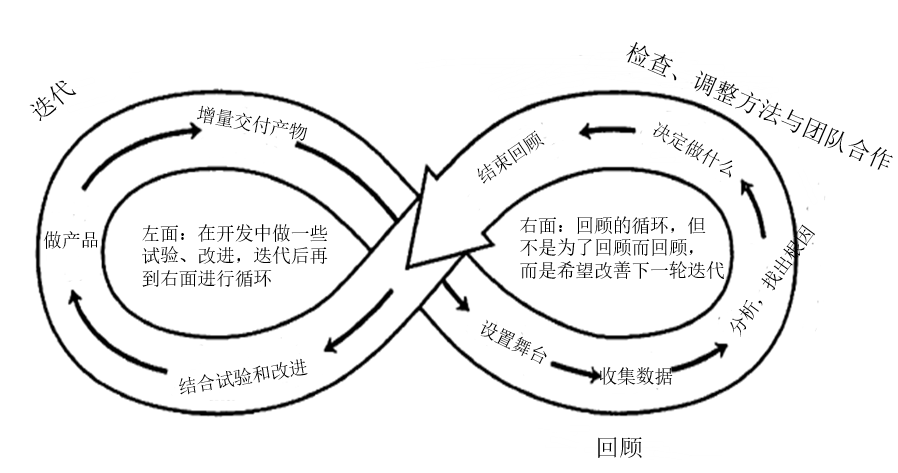
\includegraphics[width=6cm]{RetrospectiveScreenshot_2021-09-21_173119.png}

以上只是根因分析的技巧,若要团队做好迭代复盘,取得效果,还要注意以下原则。

\hypertarget{ux505aux597dux56deux987e4ux539fux5219}{%
\subsection{做好回顾4原则}\label{ux505aux597dux56deux987e4ux539fux5219}}

1. 回顾让数据提供者能即时收到反馈\\


\begin{itemize}
\tightlist
\item
  软件开发与工业生产不一样,大部分的数据必须开发人员自己收集,不能单靠机器/系统(例如:返工工作量)
\item
  如果回顾时分析根因是依据迭代数据,除了能帮助根因分析更具体外,也让团队成员有动力收集数据(因他们知道会一起分析数据)
\end{itemize}

因为软件开发是知识性工作,例如,某活动所花的工时,必须靠个人记录(具体步骤可参考`个人量化管理')

\begin{itemize}
\tightlist
\item
  但记录数据要花精力,如果不了解收集的数据,后面有什么用途,便难以维持不断收集数据的习惯
\item
  反之,当大家都清楚到迭代回顾时会一起分析团队数据,并制定改进措施,就有动力继续迭代里统计数据
\end{itemize}

2. 整个团队(所有相关干系人)参与\\
整个团队分析全局问题。例如,如果只是从测试人员的角度,他可能以为缺陷都是来自开发;需求分析人员(或产品经理)会觉得自己做得很好,因需求评审里没有什么问题被发现。但如果团队所有成员聚在一起(包括项目经理、需求、设计、编码、测试),把所有的缺陷列出来,让团队所有岗位一起分析,才可以全局看问题,才可能发现不少问题是因为需求没有明确,导致后面做出来的功能并不是客户要的。后面可扩大参与回顾的干系人,例如客户代表,可以更全面分析。\\
3. 让团队自己寻找改进方案 \\

\texttt{~必须参与一起分析、讨论,才有动力后面采取行动。}

\framebox{%
\begin{minipage}[t]{0.97\columnwidth}\raggedright
``我们团队回顾都是全部成员参加,一起讨论''某团队组长说。
以下是团队一起讨论后的根因分析结果:

%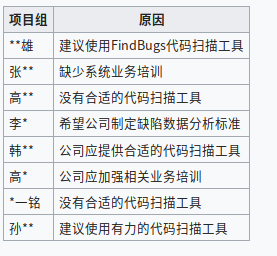
\includegraphics[width=6cm]{Screenshotfrom2023-10-3104-24-58.png}

\begin{tabular}{|c|c|c|}
\hline
项目组&原因&投票数\\
\hline
**雄&建议使用FindBugs代码扫描工具&1\\
\hline
张**&缺少系统业务培训&基1\\
\hline
高**&没有合适的代码扫描工具&2 \\
\hline
李*&希望公司制定缺陷数据分析标准&1\\
\hline
韩**&公司应提供合适的代码扫描工具&3\\
\hline
高*&公司应加强相关业务培训&2\\
\hline
*一铭&没有合适的代码扫描工具&4\\
\hline
孙**&建议使用有力的代码扫描工具&5\\
\hline
\end{tabular}

有没有看到组长提出建议使用代码扫描工具后,其他7位团队成员中4位也提类似原因?\\
所以当团队一起围着开会时,很多人都会避免提出与众不同意见,所以如果用投票方式,让大家对提出的``原因''进行投票时,票数最多的通常也是组长提出的方案(扫描工具)。
\strut
\end{minipage}}

从Asch1951群众压力实验(详见附件),看到人容易受群众压力影响(尤其当大家不认识),不敢独立表达个人看法,所以很多会议都只是项目经理一言堂,其他人只是观众,没有投入分析。为了鼓励每人畅所欲言,表达独立看法,并达到共识需要:

\begin{enumerate}
\tightlist
\item
  鼓励每人用实例讲关于质量、过程的观点/经验(寻找大家的共通点)。
\item
  鼓励每人分享个人感受、想法、满意开心/困惑的时刻(让大家相互了解)。
\end{enumerate}

\begin{itemize}
\tightlist
\item
  当大家感受到都是面对类似的问题,才会放开自己,分享个人看法。
\item
  教练的目标是让每人都有充分机会表达自己的观点。
\end{itemize}

所以在回顾时,也要想办法避免发生这种心理上的影响,导致不能真正挖掘问题的原因。所以在回顾需要大家开放,以下两方法可以减少团队压力,让大家更投入,能畅所欲言:

\begin{enumerate}
\tightlist
\item
  回顾开始时
  (设置舞台,``破冰''),用互动游戏,让团队放开顾虑,全心投入讨论
  (可参考附件里``游戏:应与否'')。
\item
  KJ分析法(详见附件):每人都有一支水笔+便利贴 ,一起找根因,每人都可以写上自己的意见。而不是传统开会方式。很多时候都只是某人讲,其他人听。无法得到团队成员充分参与。如果可以给团队自主权,他们就更能发挥、更能达到目标。\\
\end{enumerate}

如果能让每位团队成员都有充分机会表达意见,不单能集思广益,做到更好的对应方案,也能提升团队后面执行改进方案的积极性,因为一般人都会更喜欢自己的选择,这道理在两个心理实验得到验证:

\begin{enumerate}
\tightlist
\item
  Brehm1956决策影响实验(详见附件)。
\item
  粮食分配实验 (详见前面第二章附件)。
\end{enumerate}


4. 看全局,寻找大家的共同点\\
避免局部最优(Sub-optimization),避免盲人摸象,
最终希望可以全面从每个角色的视角全面分析。

某公司管理层一直非常关注度量,对各过程,包括需求、开发、测试等,都订了七八个KPI指标,并每月监控。但各个过程按指标做好不一定代表总体效果会好。
每个过程都会影响软件开发最后遗漏到客户的缺陷数,迭代回顾的时候,团队可以用缺陷排除的预测模型让团队`看见'如果代码评审排除率提升如何影响每个过程的缺陷数,不仅仅是定性的讨论分析。

例如,为什么要用`设置舞台'开始迭代回顾?(例如`应与否'是其中一种方法,详见附件),目的是让整个团队全心参与,如大家没有担心,愿意提意见,才能更全面看问题,寻找共同点,而不是辩解。

\framebox{%
\begin{minipage}[t]{0.97\columnwidth}\raggedright
例如发现大量缺陷大部分都在系统测试和验收测试才暴露,
大部分缺陷未在前面评审和单元测试发现并解除,根因分析讨论后发现单元测试没有任何要求,依赖程序员自己测。但很多时候程序员就因为时间压力都没认真去测。因为大家都忙,没有时间去深入去看,代码评审也没有发现多少问题。针对这些点大家觉得可以加强静态扫描工具,尽早发现一些语句基本问题,或重复代码等问题,减轻依赖人工查看;单元测试可以用脚本写,并规定有一定的语句覆盖率要求(例如,\textgreater{}80\%)。但如果团队只是按这些去做,没有定量化目标就很难衡量,做得够不够?不然要等到迭代最后复盘时才知道效果如何。

好比要设计一座新的80层高楼,建筑师预先用工程模型预估它防地震、防台风的能力,不要等到建好才知道有问题。团队可利用蒙地卡洛预测模型预先依据以往迭代的数据,把参数输入模型,比如每个阶段引入的缺陷数,每个阶段的缺陷排除率。首先可以利用蒙地卡洛模型,看看它出来的缺陷分布,验证是否对应以往迭代数据,预估范围是否可以覆盖以往数据。

第二步,就可以使用蒙地卡洛模型做一些实验:例如,我们估计用了静态扫描可以把代码评审的排除率从本来的10%提升到50%,团队利用蒙地卡洛模型可以预估这种搭配的各个过程的缺陷分布,我们就可以看到如果这个排除率提升的话,评审应该出发现多少缺陷,比以往提升多少。团队也可以加入利用脚本的单元测试的缺陷排除率,例如估计能从本来的排除只有20%提升到55%,看到对整个缺陷分布的变化?这样的话,我们就可以团队有下一轮迭代各个过程的缺陷预估范围参考。如果发现在代码扫描后这个缺陷数达不到本来的预期目标,便可立马采取纠正措施,不要等到最后迭代回顾时才发现未能达不到本来的预期效果。

如果有好几种方法选择,蒙地卡洛预测模型更可以帮我们做选择一个最优的最佳搭配,比如我们只是先做好评审,还是先做好单元测试,因为那些都会增加一些工作量,还是两边种方法都做,我们就可以要用蒙地卡洛以总成本最低选最佳搭配。反过来,如果没有这种蒙地卡洛工具的话,团队是很难看到每一种变化总体的效果,像盲人摸象。

因为工具可以反映过程之间的相互关系,如果我前面评审发现多了,遗漏到后面的缺陷就会减少,一层一层的关系,它利用那个缺陷排除的关系模型就可以估计总体的效果,也帮团队迭代回顾从定性改进分析,提升到定量。(如何从迭代的缺陷数据,利用蒙地卡洛预测模型,做定量分析,详见附件。)
\strut
\end{minipage}}

\hypertarget{ux56e2ux961fux8fedux4ee3ux56deux987eux6839ux56e0ux5206ux6790ux5e38ux89c1ux95eeux9898}{%
\subsection{团队迭代回顾根因分析常见问题}\label{ux56e2ux961fux8fedux4ee3ux56deux987eux6839ux56e0ux5206ux6790ux5e38ux89c1ux95eeux9898}}

\begin{enumerate}
\tightlist
\item
  没有利用缺陷数据做帕累托图分析,不清楚应针对哪一类,不清楚哪一类问题最多,导致根因分析讨论没有针对性。有些缺陷分类没有定义好,不明确或重同一缺陷可以归到几个类别,导致分析结果没有参考作用。
\item
  不清楚怎么是根因,只找到表面看到的现象,例如人经验不足,对技术不熟悉,对业务不熟悉等。没有抓到系统的根本问题。
\item
  没有量化目标,只有定性的根因分析,下轮迭代难以判断效果能否达到。
\item
  回顾时间不够。
\item
  设备、纸张、工具等未准备好。
\end{enumerate}

\framebox{%
\begin{minipage}[t]{0.97\columnwidth}\raggedright
除了教团队根因分析技巧(定性)以外,也需要展示如何使用水晶球蒙提卡罗预测模型,预估各类缺陷数范围,有了范围才可以判断最终结果是否达标,差多远。识别出哪些过程有差异,下一轮回顾才能更有针对性。如果团队想下一个迭代降低遗漏到客户的缺陷数,尽量提前用评审或测试预先发现并解决。如果仅仅提一些改进方法,比如加强评审,使用工具等,效果很有限。例如团队一般也有做评审,例如需求评审,但无法判断评审质量如何? 例如,发现四个缺陷是否足够呢?我们就可以用缺陷排除率配合蒙地卡洛模型,估计使用新提升方法后,预计的缺陷数范围,让团队立马知道缺陷数没达到预期,而不仅仅是走过程。(关于缺线排除率配合蒙地卡洛的原理,详见附件)
\strut
\end{minipage}}



以上前3点可以利用培训加强相关能力,为了确保团队能做好第一次迭代回顾,建议要之前和团队做培训。
后两点可以做好准备,预防问题发生,所以若要做好回顾,除了要理解上面4原则,也需要注意以下两条件:

\begin{itemize}
\tightlist
\item
  回顾的环境、设备: 有大白纸贴在墙上、水笔、便利贴等。
\end{itemize}

\framebox{%
\begin{minipage}[t]{0.97\columnwidth}\raggedright
有时便利贴可能太小,或字很小,原因是如果用一般的白板笔,字就太大了,如果用平常的0.5mm水笔,太细,字太小,都不合适。应该买一些比如2MM粗的水笔,才合适写便利贴。让大家可以在一到两米距离都能看得清。还有那些便利贴是不适合直接贴在普通白板上的,所以必须先从图文店买一卷比如两米宽的卷纸,用泥胶稳固在墙上;因便利贴只是上边有粘性,要在便利贴下部背面贴上一点泥胶,便不会出现便利贴下面翘起来,影响整个KJ报告看不清的情况。整个房间应该有充分的空间让大家活动,而不是那种传统一个大长座的会议室,因为越是让大家活动流动,才能投入。\\
\end{minipage}}

\begin{itemize}
\tightlist
\item
  足够的时间,起码3小时。
\end{itemize}

\framebox{%
\begin{minipage}[t]{0.97\columnwidth}\raggedright
某成都客户场景\\ 我问:现在你们团队开始做迭代回顾,团队一起分析根因,持续改善。您觉得效果如何?

研发总监:挺好,但是还是感觉他们开回顾会,耗时太长了,2个小时以上

我:因需要团队收集数据,分析,讨论下迭代措施,所以通常要3小时,熟练后会快一点,底线是改进的节省应大于回顾的投入。

高层的支持是任何改进的重要成功要素。所以首先要让管理者赞同迭代回顾能为公司带来回报(省钱),可以节省的成本(工作量)大于回顾的人力投入;也要让他理解任何改变都有个混沌的过渡期,要经过几轮回顾后,团队才能自己持续改善。
\strut
\end{minipage}}

\framebox{%
\begin{minipage}[t]{0.97\columnwidth}\raggedright
如果回顾只能1 ~ 1.5 小时的话,就不够时间让团队针对缺陷分组分类、画帕累托图做分析,没有根据实际数据分析根因,也影响到团队没有动力在后面迭代花精力去收集数据。例如,缺陷返工数据一直都非常难获取得到的,也需要在迭代根因分析时给时间团队讨论统计,所以通常1个完整的迭代根因分析回顾不会小于3小时。要做好这块如果有本地的教练可以更好控制整个回顾的节奏。不会在某一个环节耽误太多时间,也不会太长,也确保大家团队人员都全程投入讨论参与。这个我们在下一章会详细讲。
\strut
\end{minipage}}

\hypertarget{ux57f9ux8badux7b56ux5212ux4e0eux51c6ux5907}{%
\subsection{培训:策划与准备}\label{ux57f9ux8badux7b56ux5212ux4e0eux51c6ux5907}}

培训能让团队能先了解利用模拟工具量化管理的原理,也让团队为收集迭代数据做准备,所以建议先做模拟互动培训。

培训的目的:

\begin{enumerate}
\tightlist
\item
  让团队用模拟数据体验量化迭代回顾应如何进行。
\item
  知道为什么要收集缺陷和返工工作量的用途。并利用类似一般开发项目的环境的缺陷数据模拟。
\item
  收集到团队真实数据是最大的挑战,培训过程中也要团队自己讨论准备如何收集迭代的数据。因为没有数据是无法做好量化迭代回顾。
\end{enumerate}

下面是一天互动培训的时间安排:(上午是做上一章迭代回顾的互动练习,下午是使用蒙特卡洛预测模型预测下迭代的互动练习。)

%\href{文件:微信截图_20230830093612.png}{500px}

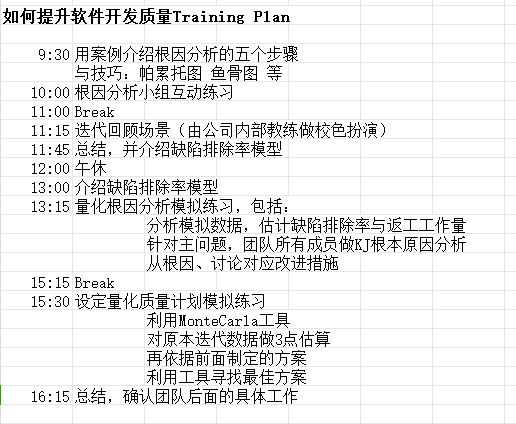
\includegraphics[width=6cm]{微信截图_20230830093612.png}

\hypertarget{ux65f6ux95f4ux5b89ux6392}{%
\subsubsection{时间安排}\label{ux65f6ux95f4ux5b89ux6392}}

如果是首次根本原因分析培训,建议先在培训当天早上做以下根因分析小组互动练习,让大家先熟悉根因分析的重点:

\begin{itemize}
\tightlist
\item
  提供模拟数据,要求团队利用帕累托图加KJ分析,找出根本原因与改进措施。
\item
  目的:让团队先感受如何基于数据,找出根本原因。
\end{itemize}

\hypertarget{ux57f9ux8badux5bf9ux8c61}{%
\subsubsection{培训对象}\label{ux57f9ux8badux5bf9ux8c61}}

\begin{itemize}
\tightlist
\item
  后面会参与试点的项目组,培训后可以把学过的在项目里实践。
\item
  所有团队角色都参加。
\end{itemize}

\hypertarget{ux51c6ux5907ux6570ux636eux8ba9ux56e2ux961fux6a21ux62df}{%
\subsubsection{准备数据,让团队模拟}\label{ux51c6ux5907ux6570ux636eux8ba9ux56e2ux961fux6a21ux62df}}

要做量化根本原因分析就必须要有数据,所以内部教练须要预先准备下面缺陷与返工工作量数据,类似一轮冲刺后的场景:

\begin{enumerate}
\tightlist
\item
  系统测试缺陷数据,建议从缺陷管理工具里抽取,40 - 60 项。
\item
  开发个人系统测试BUG返工工时统计表:那个BUG号 / 总修复工时 / 备注。
\item
  开发个人开发期间用于修复评审/单元测试返工工时统计表:那个模块 /。
  总修复工时 / 备注
\end{enumerate}

\begin{itemize}
\tightlist
\item
  打印以上的数据表,发给团队做练习时参考
\end{itemize}

例如,互动练习时,要学员利用开发人员工时表
(模拟他们迭代中用于改缺陷的工时,与评审缺陷数,与开发和修正代码的工时):

%\href{文件:缺陷表4.1.jpg}{500px}

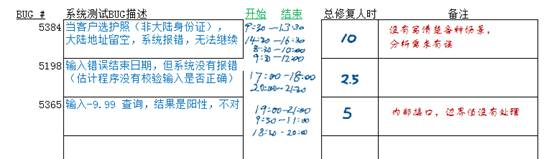
\includegraphics[width=6cm]{缺陷表41.jpg}

%\href{文件:缺陷表5.1.jpg}{500px}

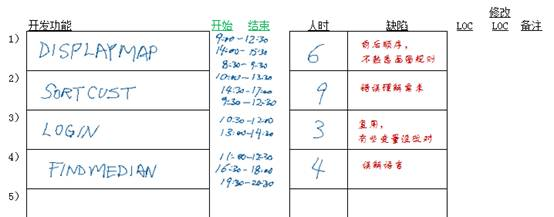
\includegraphics[width=6cm]{缺陷表51.jpg}

\hypertarget{ux51c6ux5907ux5de5ux5177}{%
\subsubsection{准备工具}\label{ux51c6ux5907ux5de5ux5177}}

\begin{itemize}
\tightlist
\item
  分2-4组,6-8人一组,,需要有一个大而光亮的会议室,
  方便小组互动,大白板和架子,各种颜色的水笔,墙壁可以贴上小组的白纸。
\item
  教练提供有水晶球工具的笔记本电脑。
\end{itemize}

\hypertarget{ux4f7fux7528ux4e8cux516bux539fux5219ux4e0ekjux5206ux6790ux6839ux56e0ux5b9eux4f8b}{%
\subsection{使用二八原则与KJ分析根因实例}\label{ux4f7fux7528ux4e8cux516bux539fux5219ux4e0ekjux5206ux6790ux6839ux56e0ux5b9eux4f8b}}

\hypertarget{ux516cux53f8ux80ccux666f}{%
\subsubsection{公司背景}\label{ux516cux53f8ux80ccux666f}}

多年来,这家公司一直做医疗IT解决方案,门槛很高,不仅要懂IT,也要懂行业知识。医院或医疗机构都对质量有要求。\\
工作压力也很大 ------
去年业务扩展很快,除了要增加软件产品数量以外,也非常注意产品质量。
例如,公司用系统统计客户反馈的缺陷。要求过程改进小组,按月统计客户反馈的缺陷,看是如何逐步到得到改进、不断完善。因员工人数快速增加,公司也注重控制成本,如研发成本。

\hypertarget{ux4eceux9879ux76eeux51b2ux523aux7684ux56deux987eux590dux76d8ux5f00ux59cb}{%
\subsubsection{从项目冲刺的回顾复盘开始}\label{ux4eceux9879ux76eeux51b2ux523aux7684ux56deux987eux590dux76d8ux5f00ux59cb}}

质量经理把我引到回顾复盘现场,技术总监(高层)也参加,测试人员投影了本次迭代的缺陷分析,展示下面2个缺陷分布图
:

\begin{itemize}
\tightlist
\item
  开发人员排名(最多的排头)
\item
  按模块来区分(最多的排头)
\end{itemize}

团队组长便按照缺陷的严重程度询问每位开发人员 -\/- 是否知道怎么修改?\\
大家都说知道了。组长要求大家提出问题,如果没有问题就准备散会。

我问:大家好,你们有没有兴趣做个小实验。
后面让我们暂时抛开自己本身是什么岗位。
大家一起看看有哪些地方能减少缺陷?

例如,除了按照人员与模块区分。 我们可否把缺陷简单按下面类型分组 :
需求/设计/编码 ?

他们就让测试人员,展示本冲刺发现的34个缺陷,让大家逐一讨论,找出缺陷是源自哪过程
,最后把总数写在白板上:

%\href{文件:DefectsBySourceScreenshot_2021-09-20_155232.png}{400px}

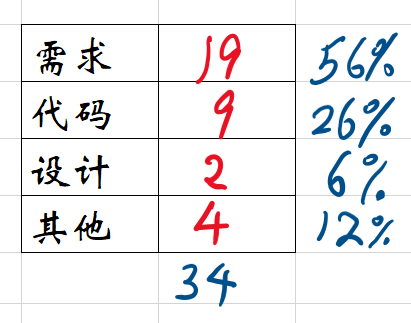
\includegraphics[width=6cm]{DefectsBySourceScreenshot_2021-09-20_155232.png}

让我们看看是怎么分布? 为什么这类缺陷最多呢?大家估计背后是什么原因?
针对需求(最多的类别),我辅导团队利用KJ方法{[}详见附件{]},识别主因。最终汇总成以下结果:\\
%\href{文件:!!reqKJfinal微信图片_20210920125228.jpg}{400px}

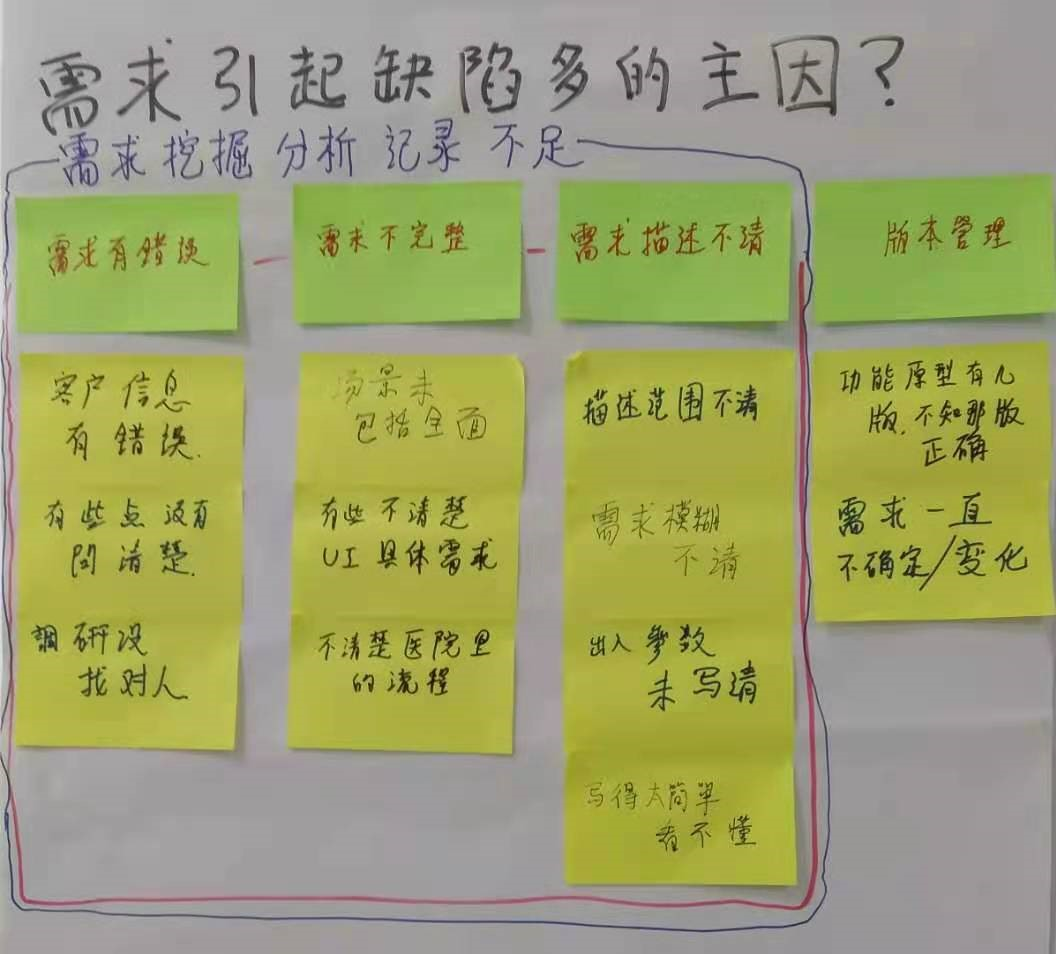
\includegraphics[width=6cm]{!!reqKJfinal微信图片_20210920125228.jpg}

\hypertarget{ux5206ux6790ux95eeux9898---ux6839ux56e0---ux884cux52a8}{%
\subsubsection{分析问题 - 根因 -
行动}\label{ux5206ux6790ux95eeux9898---ux6839ux56e0---ux884cux52a8}}

我:针对我们刚才一起找出的主因,根本原因是什么?
如何可以避免同类缺陷再发生?

总监:要加强对需求人员的培训,提高他们的能力。\\
我年初已察觉到确实很多需求没有表达清楚。
导致开发出来的东西不符合客户要求,或不是客户要的。

总监接下来说:

\framebox{%
\begin{minipage}[t]{0.97\columnwidth}\raggedright
我见过以下用户故事:

患者或他的家属能容易找到他选择的服务。\\
理由:他们熟悉网上购物,习惯了方便和快速的响应时间。\\
我问需求人员怎样才算容易找到,验收标准?

我估计她记得我说过需求必须可测量,她想了一会,说验收标准:``普通患者能够在6秒钟内通过不超过3个动作定位任意一项服务。''

我说如果把`普通患者'改为`90\%以上的患者'更好。

必须把模糊,有二义性的需求变成可以测量。

所以不能仅仅说 ,“新功能很酷,很创新",
而应明确验收标准为:引入了新功能的3个月之内,60\%的用户应该用它来完成规定的工作。75\%以上的用户对产品表示赞许。

所以3个月前,我已经开始 准备正式规划产品经理与需求分析师岗位,
要经过挑选,考试,然后培训,达标才能正式上岗。
本来计划2周后会正式公告,现在既然你们问到,我就预告一下。\strut
\end{minipage}}

我:既然高层已经有长远的规划,我们团队就应该针对下一个冲刺,我们可以做到的事情。\\
团队:我们每个岗位都已经尽了全力,没有什么可以做了。\\
我:你们有做评审吗?如需求,设计评审。\\
团队:有。\\
我:需求评审发现多少缺陷,设计评审发现多少?\\
团队:好像2、3个。\\
我:发现什么问题?\\
团队:记不清了,当时直接就修改了。\\
我:请问评审总共花了多少时间?多少人参加?\\
团队:我们6个人,那次评审大概用了接近2小时。\\
我:2小时?\\
团队:我们不仅仅发现需求问题,也一起讨论如何修改\\
我:如果评审只找缺陷、记录,应不会超过1小时,如果大家事前做好准备,估计可能半小时可以完成。所以通常检查(Inspection
)不会当场讨论如何修改。\\
我接着说:我们刚才分析系统测试缺陷,不是识别出超过一半是源自需求吗?为什么我们不能在评审时预先发现?你们觉得可以下一个冲刺,评审时可以发现更多缺陷吗?\\
我立马用5分钟与大家分享有效评审能提高产品质量,降低成本的例子。

团队:估计应该可以,但不知道怎么做?\\
我:你们评审有检查清单吗?\\
团队:没有。\\
我:清单可以帮助我们吸收以往的经验,避免以后同类问题再发生。例如刚才我们都识别了跟需求挖掘/分析/记录不足相关的具体问题吗?
可否利用这些,更新评审检查单的检查项,提醒我们要避免同类问题。如果大家同意,我们现在就行动。我们要改进便要制定目标,例如计划下次需求评审、系统测试等各过程发现的缺陷数。这些目标你们可以下周一策划2周冲刺时定。

组长安排了小李更新检查单。准备在下次评审前与需求文档,预先发给参评人员。

我:谢谢大家,我没有其他要说了,下次回顾,我或总监会来参加,看看冲刺的效果。

要利用根本原因分析做改进,必须有数据,
也需要有机会立马实验改进方法,评判效果,
所以迭代回顾(或复盘)是做根本原因分析的最佳时机。
但很多团队只在迭代回顾时讨论如何解决迭代暴露的缺陷与相关职责分工,没有探索根本原因,
和如何能避免同类问题再发生。

\hypertarget{ux7ecfux9a8cux6559ux8bad}{%
\subsection{经验教训}\label{ux7ecfux9a8cux6559ux8bad}}

很多开发人员虽然编码/测试很有经验,但不熟识统计分析,蒙地卡洛模拟等,所以整个培训需要有内部教练辅助他们怎么利用那些工具技巧去分析数据。团队只是提供数据和分析结果,不一定要很了解里面的数据分析,但必须真正了解根因分析,所以我们培训会以根因分析开始,用前面的丰田故事,日本绅士俱乐部原因分析故事。让大家了解根本原因分析的重点。然后给小组前面的机场延误数据,让他们利用KJ模拟方式和帕累托图,自己动脑筋找出根因,我们的经验:越多互动练习,他们就越感兴趣,越主动参与。所以如果时间有限,尽量可以压缩讲理论的部分,甚至要他自己先阅读了解,大部分时间让他利用数据分析根因。有了这个基础就可以进入第二部分,利用内部教练准备好的几十条系统测试缺陷,要他们按缺陷排除的方式,找出缺陷的主要来源,并估计返工工作量,再利用蒙地卡洛模拟估计每一个过程的缺陷范围。经过培训,他们便可以在下一个迭代回顾时用同样思路,分析自己的迭代数据,找出根因并制定下一轮迭代的纠正措施。培训结束前,内部教练在总结时要求大家团队讨论后面有什么方式可以收集到做迭代回顾所需要的数据,例如缺陷数、返工工作量等。

\hypertarget{ux7ed3ux675fux8bed}{%
\subsection{结束语}\label{ux7ed3ux675fux8bed}}

要做好迭代回顾,首先必须得到高层的支持,并取得所需的资源与时间。策划与培训是成功的第一步。因一般团队没有回顾与根因分析的概念,教练如何现场辅导也很重要。

下章会分享如何在回顾中的注意事项和如何持续。

\hypertarget{ux9644ux4ef6}{%
\section{附件}\label{ux9644ux4ef6}}

\hypertarget{ux6e38ux620fux5e94ux4e0eux5426}{%
\subsection{游戏:应与否}\label{ux6e38ux620fux5e94ux4e0eux5426}}

在迭代回顾中使用。

\hypertarget{ux76eeux7684}{%
\subsubsection{目的}\label{ux76eeux7684}}

帮助建立有效沟通的思维模式。帮助参与者抛开指责和判断,以及对指责和判断的恐惧。

\hypertarget{ux6240ux9700ux7684ux65f6ux95f4}{%
\subsubsection{所需的时间}\label{ux6240ux9700ux7684ux65f6ux95f4}}

8 \textasciitilde{} 12分钟,取决于小组的大小。

\hypertarget{ux63cfux8ff0}{%
\subsubsection{描述}\label{ux63cfux8ff0}}

在描述这些模式之后,参与者讨论这些沟通模式的意义。

\hypertarget{ux6b65ux9aa4}{%
\subsubsection{步骤}\label{ux6b65ux9aa4}}

\begin{enumerate}
\tightlist
\item
  将注意力集中在``应与否''(见下图),并简要阅读。
\item
  组成小组,每组不超过4人。要求每组用一对词来定义和描述。如果有4对以上的词对/组,如果有多个组有相同的词组对,也可以。
\item
  让每个小组讨论他们的2个单词的意思和它们所代表的行为。让他们描述各自对团队和回顾的影响。
\item
  每个小组向整个小组汇报他们的讨论情况。
\item
  询问大家是否愿意使用左面的方式。
\end{enumerate}

\href{文件:_游戏1应与否1.png}{500px}

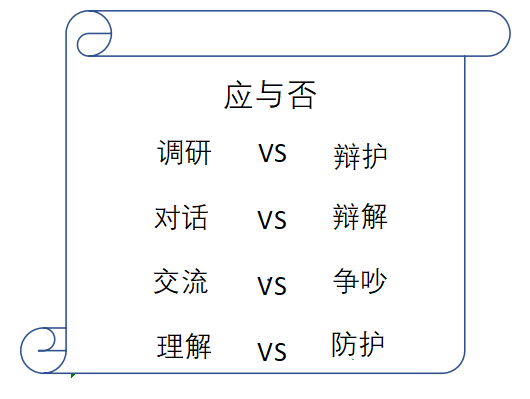
\includegraphics[width=6cm]{游戏1应与否1.png}

\hypertarget{ux7528ux89d2ux8272ux626eux6f14ux4e3aux505aux597dux56deux987eux6253ux57faux7840}{%
\subsubsection{用角色扮演为做好回顾打基础}\label{ux7528ux89d2ux8272ux626eux6f14ux4e3aux505aux597dux56deux987eux6253ux57faux7840}}

学员用各种角色扮演什么是吵架、什么是交流,让观众和表演者更能感受到量化回顾先要有对事不对人的心态:


%1498.png\textbar{}对话 1499.png\textbar{}辩解

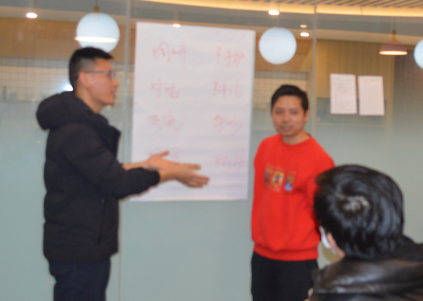
\includegraphics[width=6cm]{1498.png}\textbar{}对话 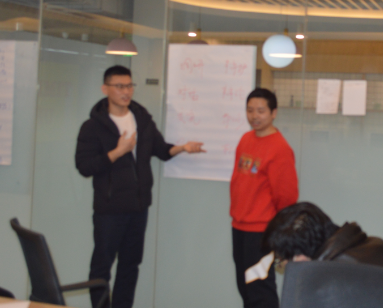
\includegraphics[width=6cm]{1499.png}\textbar{}辩解

\hypertarget{ux5982ux4f55ux5728ux8fedux4ee3ux56deux987eux65f6ux5206ux6790ux7f3aux9677ux6570ux636eux5f97ux51faux9884ux6d4bux6a21ux578bux53c2ux6570}{%
\subsection{如何分析缺陷数据得出预测模型参数,出分布图}\label{ux5982ux4f55ux5728ux8fedux4ee3ux56deux987eux65f6ux5206ux6790ux7f3aux9677ux6570ux636eux5f97ux51faux9884ux6d4bux6a21ux578bux53c2ux6570}}

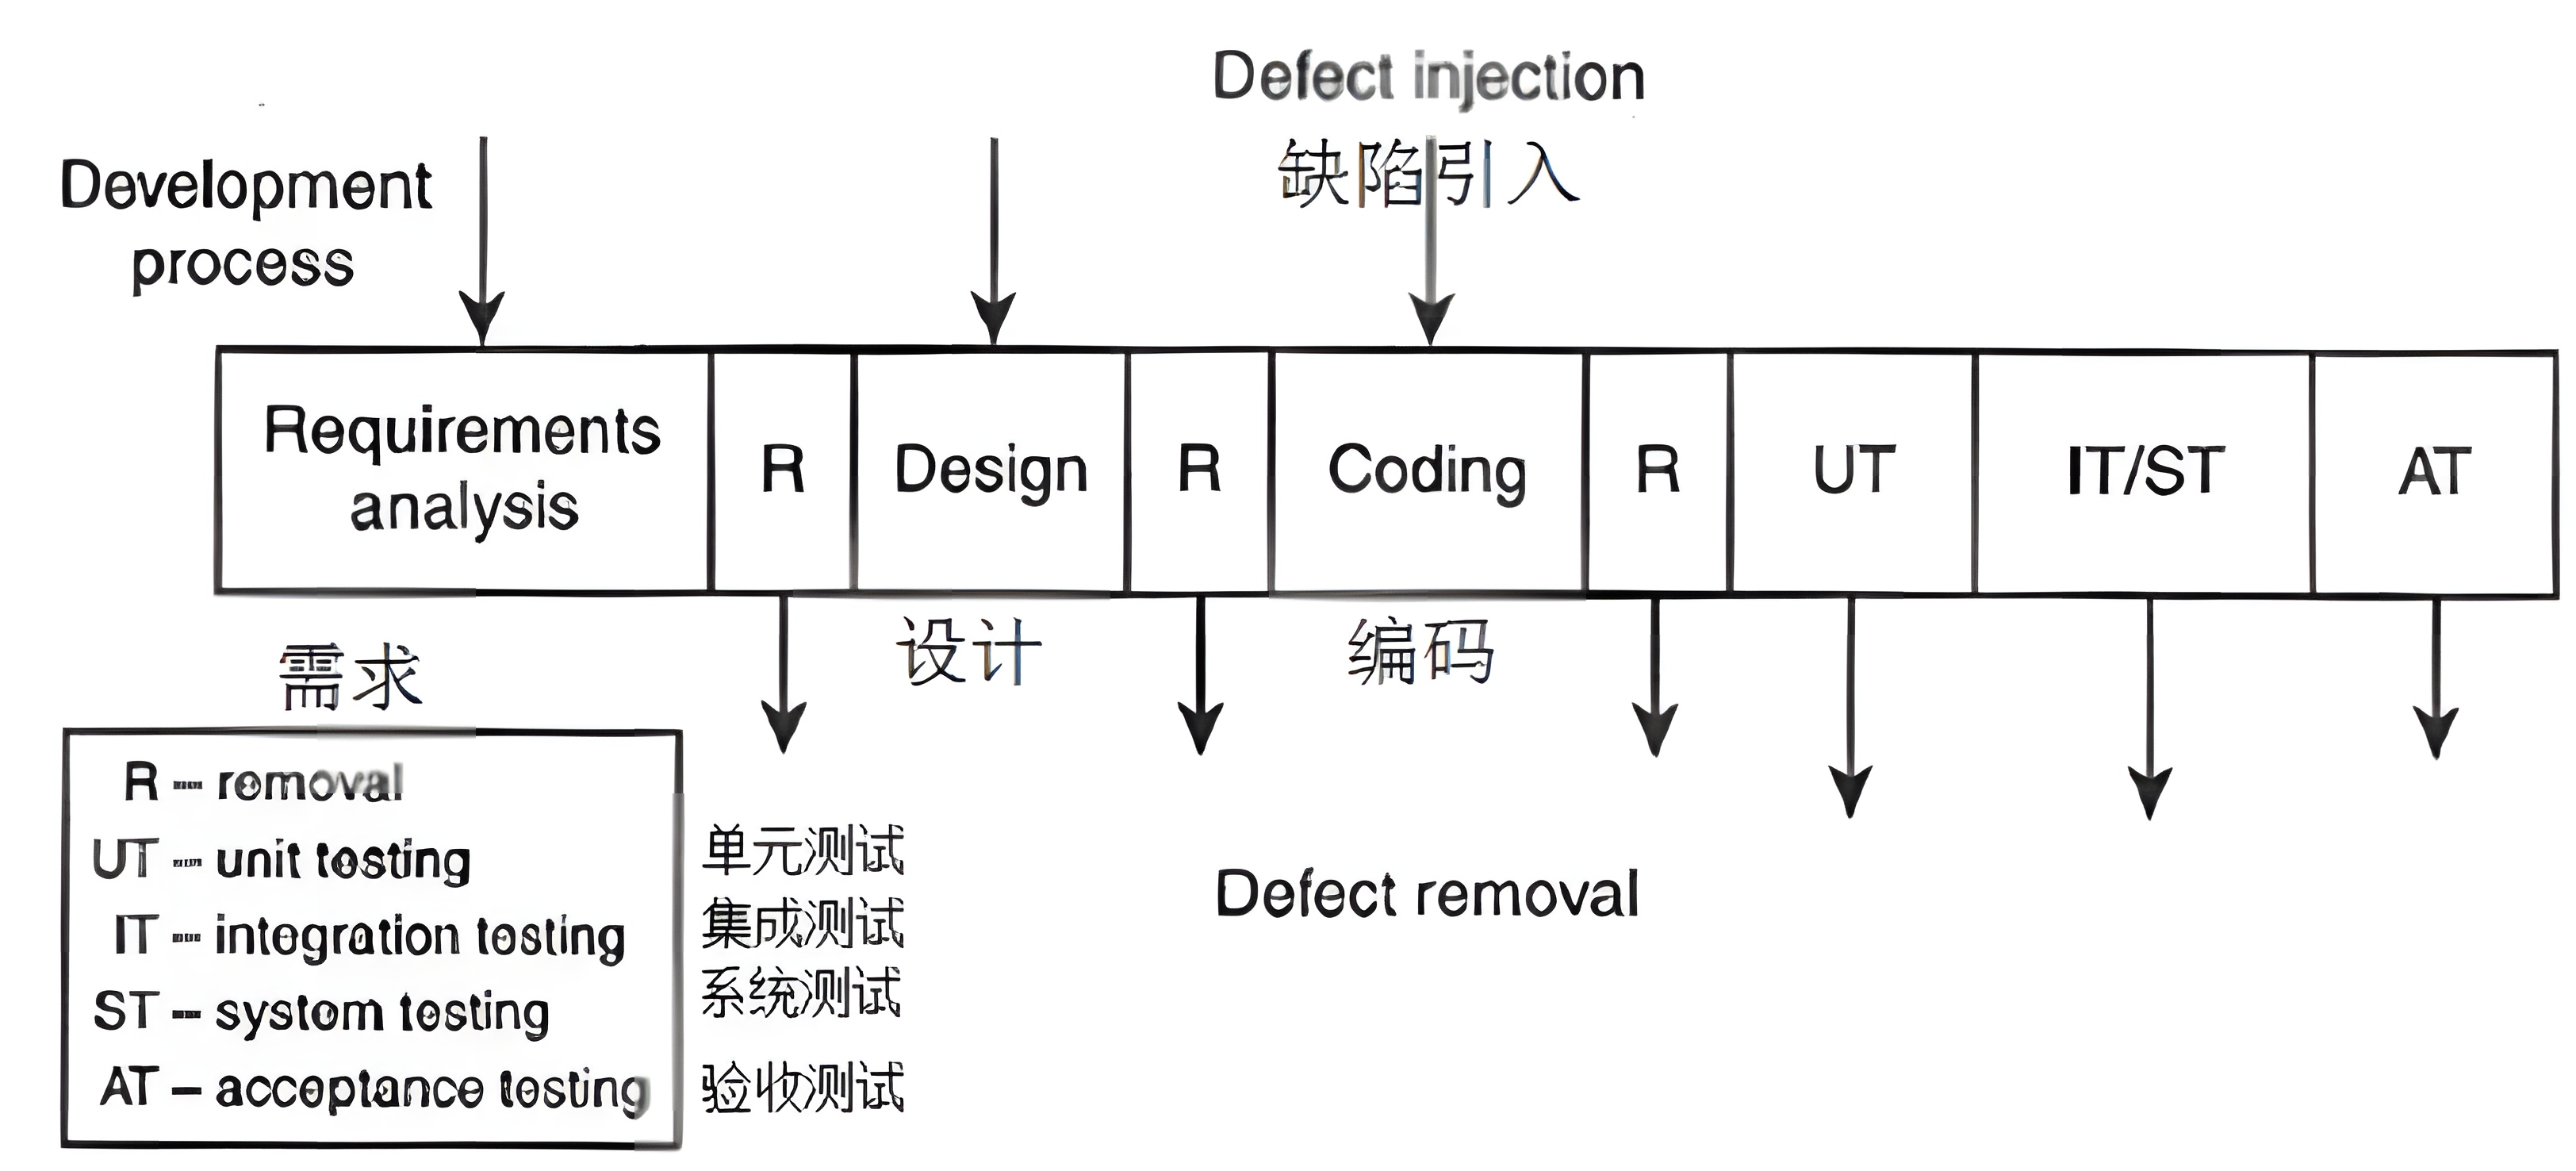
\includegraphics[width=6cm]{Jalote_emm_71-1.jpg}

需求、设计、编码后都会评审/测试来排除缺陷,但仅仅做评审/测试不一定能确保质量。因为最终验收缺陷数取决于每个步骤能否有效排除当前的缺陷。\\

可以用缺陷排除率(Defect Removal Efficiency DRE) 来衡量测试或评审的效率:


%\href{文件:Ma3_1.0.png}{文件:Ma3 1.0.png}

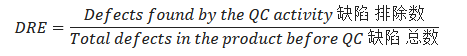
\includegraphics[width=6cm]{Ma3_10.png}

有些人会认为尽早发现并解决缺陷

对质量肯定好,但会耗费工作量,增加项目成本,老板不一定愿意。

其实是反过来,如能在前面预先发现并修正缺陷,

便能减小后面测试和修改缺陷的工作量,

最终只会减少总项目工作量。

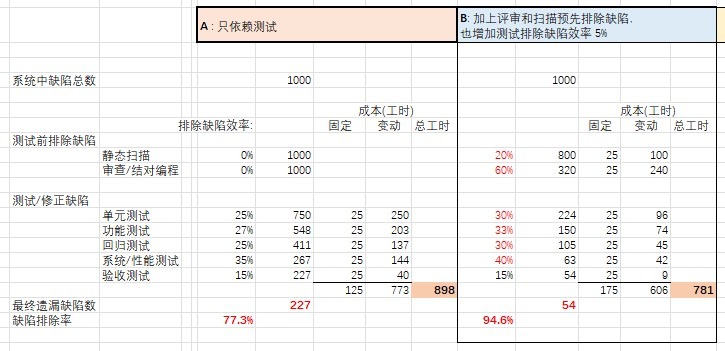
\includegraphics[width=6cm]{AR1FixVarCostScreenshot_2022-12-10_144400.jpg}

比较以上两种策略的质量成本(COQ)就能看出:

\begin{itemize}
\tightlist
\item
  增加测试前扫描与审查,并加大测试效率,不仅减少最终缺陷数到54(对比227),也降低总质量成本(总人时)
\end{itemize}

\framebox{%
\begin{minipage}[t]{0.97\columnwidth}\raggedright
假设:每项任务的固定成本都是25人时;测试前的缺陷修复:每缺陷用
0.5人时;测试缺陷修复,上面计算假定每缺陷用1人时,详见下表:

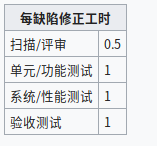
\includegraphics[width=6cm]{Screenshotfrom2023-11-0302-29-26.png}
%Screenshotfrom2023-11-0302-29-26.png

%通常测试里的缺陷修复每缺陷不只1人时,例如,在验收阶段时可能要用20人时;我通常会打开这XLS
%表,填上客户的估计值。从上表看到,即使用最少的1人时来算,还是不亏。

\begin{itemize}
\tightlist
\item
  通常测试里的缺陷修复每缺陷不只一人时,例如,在验收阶段时可能要用20人时;我通常会打开这XLS
表,填上客户的估计值。从上表看到,即使用最少的1人时来算,还是不亏。
\end{itemize}

\strut
\end{minipage}}

因为缺陷已经提前被排除系统测试的缺陷减少,测试阶段的工作量减少大于前面扫描评审上的投入。

可以进一步利用COQ概念,增加早期预防缺陷措施,如用原型与客户交流,做好需求调研,进一步减少缺陷,和成本。
例如,使用原型与场景与客户挖掘需求,可进一步把缺陷降到43,也降低总质量成本:

%\href{文件:est缺陷表3.jpg}{600px}

\includegraphics[width=10cm]{est缺陷表3.jpg}\\

\texttt{注:你可能会质疑使用原型方法不只25人时,但即使加大到100人时,还是不亏。因它能预防缺陷,整体缺陷数下降20\%,使总质量成本下降超过100人时。}


下面我们介绍一下怎么从引进量化管理来提高开发质量:\\
\#设定量化目标。例如希望最终遗漏到验收发现的缺陷数降多少?

\begin{enumerate}
\tightlist
\item
  并设定中间阶段目标缺陷数,从而预测能否达到最终目标,不要等到最后才知道不满足
\end{enumerate}

可用缺陷排除率来判断每一个过程的质量:\\
如果要最终质量好,缺陷排除率就要高。但计算缺陷排除率,必须要等到整个开发完成才可以计算,我们可以建立一个预测模型,模拟这个过程:\\
需求会引入缺陷,然后需求评审排除缺陷等等。把各引入缺陷数,排除率输进蒙地卡罗预测模型,然后使用它估计每个阶段的缺陷数量范围。

Infosys PCB的缺陷分布(Defect Distribution in Infosys's PCB)

%Screenshotfrom2023-10-1023-46-22.png

%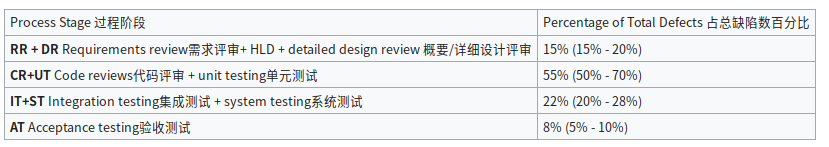
\includegraphics[width=6cm]{Screenshotfrom2023-10-1023-46-22.png}

\begin{tabular}{|c|c|}
\hline
Process Stage 过程阶段&Percentage of Total Defects 占总缺陷数百分比\\
\hline
RR + DR Requirements review需求评审+ HLD + detailed design review 概要/详细设计评审&15\% (15\% - 20\%) \\
\hline
CR+UT Code reviews代码评审 + unit testing单元测试&55\% (50\% - 70\%) \\
\hline
IT+ST Integration testing集成测试 + system testing系统测试&22\% (20\% - 28\%)  \\
\hline
AT Acceptance testing验收测试&8\% (5\% - 10\%) \\
\hline
\end{tabular}

如果我们按上面 infosys
公司的各阶段缺陷利率百分比,设计与需求排除缺陷15\%,代码评审与单元测试55\%,集成/系统测试22\%,验收测试8\%,下面按缺陷总数为100,
得出算出设计与需求排除共15缺陷, DR+RR=15,CR+UT=55, IT+ST=22,
AT=8,求出各阶段的缺陷输入与缺陷排除率,把参数输入蒙地卡洛预测模型:\\
表D1:\\
%\href{文件:1113correctEgScreenshot_2021-11-13_212414.png}{400px}
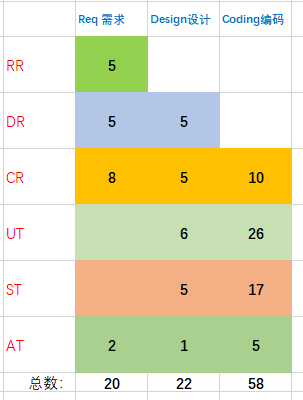
\includegraphics[width=6cm]{1113correctEgScreenshot_2021-11-13_212414.png}

%\href{文件:1113corrDreScreenshot_2021-11-13_212509.png}{600px}
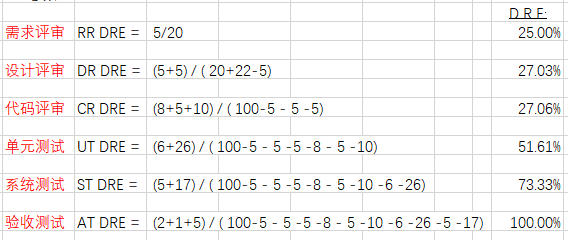
\includegraphics[width=6cm]{1113corrDreScreenshot_2021-11-13_212509.png}

得出下面的表,缺陷分布是中间最高头尾低,右面与左面不同,有条长尾巴,类似估算软件开发项目工作量的
Rayleigh 曲线。

%\href{文件:jalote_emm_7.2.png}{500px}
\includegraphics[width=6cm]{jalote_emm_72-1.jpg}

模型假定每个阶段的缺陷排除率都比较稳定,在某个范围之内,不同阶段引入的缺陷也在一定范围之内。蒙地卡洛模型让我们可以设定缺陷排除率和缺陷输入数量的波动范围,预测各阶段缺陷排除分布范围,不仅仅看单点数(前面在第三章里介绍过如何使用蒙地卡洛模型做三点估算)。

\hypertarget{ux57f9ux8badux5bf9ux8c61}{%
\subsubsection{使用水晶球蒙地卡罗模型实例}\label{ux57f9ux8badux5bf9ux8c61}}

\begin{itemize}
\tightlist
\item
  在模型参数输入部分输入估计对应缺陷排除百分比的上下限与均值,工作量也类似。例如,代码走查的缺陷排除率是55%;评审工作量(不包含修正缺陷)为20人时。如代码正式审查排除率是85%,但工作量会增加到35人时 。如下图:

\end{itemize}

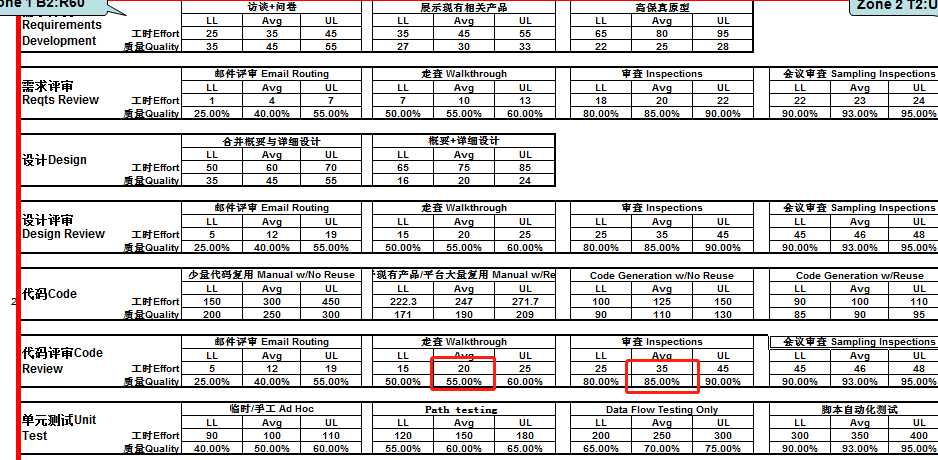
\includegraphics[width=6cm]{微信截图_20211027011246.png}

\begin{itemize}
\tightlist
\item
  模型会自动按输入的最大最小值用PERT方程式计算标准差,变成分布(正态(Normal)分布、),水晶球模型会依据 Decision 格的数字选取对应的分布,

\end{itemize}

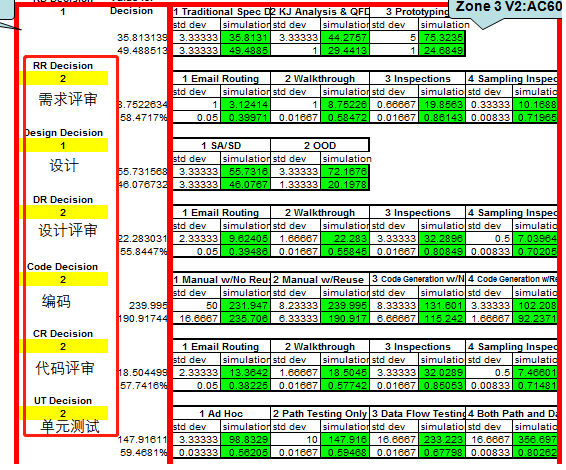
\includegraphics[width=6cm]{微信截图_20231027140307.png}

\begin{itemize}
\tightlist
\item
  成本参数:例如 Quality 行:修复一个系统测试发现的缺陷,平均要用8000元,最高9200,最低6800。例如 Effort 行:平均人时成本,平均是600元,最750,最低500。水晶球模型就会依据输入依据三角形分布估算单位成本的分布,放在绿格里。
\end{itemize}

\includegraphics[width=6cm]{微信截图_20231027140341.png}

\begin{itemize}
\tightlist
\item
  估算质量成本:水晶球会依据质每过程的缺陷分布和单位成本分布,预估质量成本的分布。例如这例子是需求评审用审查(2),设计评审用走查(2) ,代码评审也用走查(2),单元测试是手工(1),系统测试估计走3轮(2),验收测试预计走3轮(2)的预估分布结果。(括号里的数字代表在模型参数表里那一栋,从1至4。如想了解水晶球如何把每个过程”加”起来,详见‘三点估算’附件:蒙特卡洛模拟)
\end{itemize}

\begin{itemize}
\tightlist
\item
  模型经过 10,000 次模拟得出质量成本分布,和过程的缺陷分布与范围(90\%置信区间)
\end{itemize}

\hypertarget{asch-1951-ux7fa4ux4f17ux538bux529bux5b9eux9a8c}{%
\subsection{Asch 1951
群众压力实验}\label{asch-1951-ux7fa4ux4f17ux538bux529bux5b9eux9a8c}}

%\href{文件:Asch0Screenshot_2022-07-09_161023.jpg}{150px}
\includegraphics[width=6cm]{Asch0Screenshot_2022-07-09_161023.jpg}

问题:\textbf{请问右面那条线 (A、 B、 C) 的长度最接近左面线的长度?}

%\url{文件:Asch2Screenshot.2.png}
\includegraphics[width=6cm]{Asch2Screenshot2.png}

实验设计:\textbf{随机邀请几位志愿者(包括你)
参加,实验之前与(除了你以外)所有人预先说好,都选A,并且要假装成经过深思熟虑。实验时,你是最后一位作答。}

结果:

\begin{itemize}
\tightlist
\item
  有群众压力时,大概\textbf{37\%}会从众选择错误答案
  (虽然不同人有差异,但总体只有\textbf{25\%}能坚持自己的正确答案。)
\item
  个人自己作答,接近100\%选对,错误率\textbf{少于1\%}。
\end{itemize}

影响因素:

\begin{itemize}
\tightlist
\item
  前面选择错误答案的人数越多,错误率越高:
\end{itemize}

\begin{enumerate}
\tightlist
\item
  一位:接近0\%答错
\item
  两位:大概14\%
\item
  三位: 32\%(详见下图)
\end{enumerate}

%\href{文件:Asch3Screenshot_2022-07-08_201341.1.png}{500px}
\includegraphics[width=6cm]{Asch3Screenshot_2022-07-08_2013411.png}

\begin{itemize}
\tightlist
\item
  如果前面有一位``战友''选了正确答案,你的错误率就显著降低(大约原本水平的1/4,看下图黄线),并让你感到与他更亲切。
\end{itemize}

%\href{文件:Asch4Screenshot_2022-07-08_201502.1.png}{500px}
\includegraphics[width=6cm]{Asch4Screenshot_2022-07-08_2015021.png}

\begin{itemize}
\tightlist
\item
  尴尬场景(例如迟到),你的错误率会更高。

  \begin{itemize}
  \tightlist
  \item
    实际你没有晚到,只是让你觉得确实迟到了,觉得尴尬。
  \end{itemize}
\item
  如果不是要你说出答案,而是让你把答案写在纸上,错误率会降低1/3。
\end{itemize}

\hypertarget{brehm-1956-ux51b3ux7b56ux5f71ux54cdux5b9eux9a8c}{%
\subsection{Brehm 1956
决策影响实验}\label{brehm-1956-ux51b3ux7b56ux5f71ux54cdux5b9eux9a8c}}

\textbf{实验设计}:

\begin{enumerate}
\tightlist
\item
  提供10多种不同礼物,包括台灯、多士炉、挂钟、收音机等。
\item
  请你按自己喜好对礼物排序
  。例如最喜欢的选一,如果同样喜欢两件礼物,可以不分高低,写同一个数字。
\item
  让你从两件同样喜好的礼物,让你选其中一件,让你拿走。
\item
  但在你离开之前,请你再对所有礼物按喜好排序。
\end{enumerate}

\textbf{结果}:

\begin{itemize}
\tightlist
\item
  绝大部分人都会抬高自己选择拿走的那一件礼物排序,调低非选择的那件礼物排序。
\item
  但如果不是自己选择,而是由老师选好给你,你后面的礼物排序就没有变化。
\end{itemize}

\textbf{结论}:

\begin{itemize}
\tightlist
\item
  人都会觉得自己的选择比较好。
\item
  例如选大学、选汽车、选伴侣。如果是由你自己决定选择(非被安排),你会不会都会觉得自己的选择较好。
\end{itemize}

\hypertarget{kjux5206ux6790ux65b9ux6cd5ux6b65ux9aa4}{%
\subsection{KJ分析方法步骤}\label{kjux5206ux6790ux65b9ux6cd5ux6b65ux9aa4}}

\includegraphics[width=6cm]{Kj1Screenshot2023-11-01133052.jpg}

\emph{一种头脑风暴方法,每人把自己想法写在便利贴上,一起轮流把所有便利贴排放分组}

\includegraphics[width=6cm]{微信图片_20231027091622.jpg}

\includegraphics[width=6cm]{微信图片_20231027091728.jpg}

\begin{description}
\item[]
\begin{description}
\tightlist
\item[]
\end{description}
\end{description}

\begin{enumerate}
\tightlist
\item
  把主题以问题形式写在大白纸的头顶。
\item
  把相关的事实写在便利贴上面,用黑色。
\item
  搜集相关的事实,如果是一组人的话,分散到不同人手上。
\item
  (团队)查看描述是否不清楚,是否要整理?
\item
  每人轮流把相关的便利贴组合在一起。
\item
  当每人都已经调整过便利贴组合后,一起把每一组便利贴加上一个题目,用红色标识。
\item
  红色的标题下包含相关事实的内容。
\item
  把相关的红色题目(最好不超过3个)组合在一起。
\item
  给这大组一个题目 -- 蓝色。
\item
  在题目下放上相关的红色小组。
\item
  把蓝色的题目和剩下红色的小组或单独没有分类的便利贴都在墙上放好,也可以用一些箭头描述它们的因果关系。

\end{enumerate}


%\href{文件:KJ_1.0.png}{600px}
\includegraphics[width=6cm]{KJ_10.png}

\hypertarget{ux6c34ux6676ux7403ux8499ux7279ux5361ux6d1bux9884ux6d4bux6a21ux578b}{%
\subsection{水晶球蒙特卡洛预测模型}\label{ux6c34ux6676ux7403ux8499ux7279ux5361ux6d1bux9884ux6d4bux6a21ux578b}}

\begin{itemize}
\tightlist
\item
  在模型参数输入部分输入估计对应缺陷排除百分比的上下限与均值,工作量也类似。例如,代码走查的缺陷排除率是55%;评审工作量(不包含修正缺陷)为20人时。如代码正式审查排除率是85%,但工作量会增加到35人时 。如下图:
\end{itemize}

%\href{文件:微信截图_20211027011246.png}{450px}

\includegraphics[width=6cm]{微信截图_20211027011246.png}

\begin{itemize}
\tightlist
\item
  模型会自动按输入的最大最小值计算标准差,变成分布(如:正态(normal)分布、三角形(triangular)分布),水晶球模型会依据黄格里的数字选取对应的分布,
\end{itemize}

%\href{文件:微信截图_20211027011403.png}{450px}

\includegraphics[width=6cm]{微信截图_20231027140307.png}

\begin{itemize}
\tightlist
\item
  成本参数:例如 Quality 行:修复一个系统测试发现的缺陷,平均要用8000元,最高9200,最低6800。例如 Effort 行:平均人时成本,平均是600元,最750,最低500。水晶球模型就会依据输入依据三角形分布估算单位成本的分布,放在绿格里。
\end{itemize}

%\href{文件:微信截图_20211027012006.png}{450px}

\includegraphics[width=6cm]{微信截图_20231027140341.png}

\begin{itemize}
\tightlist
\item
  估算质量成本:水晶球会依据质每过程的缺陷分布和单位成本分布,预估质量成本的分布。例如这例子是需求评审用审查(2),设计评审用走查(2) ,代码评审也用走查(2),单元测试是手工(1),系统测试估计走3轮(2),验收测试预计走3轮(2)的预估分布结果。(括号里的数字代表在模型参数表里那一栋,从1至4。如想了解水晶球如何把每个过程”加”起来,详见‘三点估算’附件:蒙特卡洛模拟)
\end{itemize}

\begin{itemize}
\tightlist
\item
  模型经过 10,000 次模拟得出质量成本分布,和过程的缺陷分布与范围(90\%置信区间)
\end{itemize}

%\includegraphics[width=6cm]{StartQUA95.PNG}
%1011


\chapter{实施与维护} % Introduction chapter suppressed from the table of contents

\hypertarget{ux51c6ux5907ux8fedux4ee3ux56deux987e-qa}{%
\subsection{准备迭代回顾
Q\&A}\label{ux51c6ux5907ux8fedux4ee3ux56deux987e-qa}}

两个月前,为北京某企业做差距分析,发现大量缺陷在系统测试才被发现,建议加强迭代回顾根因分析。质量经理便开始尝试内部推动,并在两周前做了一次团队回顾辅导。

\hypertarget{ux505aux597dux73b0ux573aux8f85ux5bfc}{%
\subsubsection{做好现场辅导}\label{ux505aux597dux73b0ux573aux8f85ux5bfc}}

质量经理:我们计划下周三就会与另一项目组做迭代回顾,他们团队共7-8人,2周前与另一团队使用便利贴做根因分析,确实能听到更多不同的声音。应如何准备好,让今次这团队能放开并做好根因分析?\\
我:让我分享一下我的相关经验:\\

\framebox{%
\begin{minipage}[t]{0.97\columnwidth}\raggedright
如果他们没有学过根因分析,应先用15分钟介绍根因分析的主要元素(可用绅士俱乐部案例),然后立马请他们分两组,使用机场延误数据做45分钟互动练习。
(因利用数据,动脑筋,是最佳学习方式。因大家都坐过飞机,也遇过延误,应能理解机场的大概情况,所以不需要用实际团队缺陷数据。)

练习过程中,我只会定时提醒时间(需要在45分钟后跟管理层汇报),有时候在做练习时,学生会问我,''我做对不对啊?是否做错?``除非他们犯了基础错误(例如,用电脑打帕里托图,或只是按延误数据被一条按数字从最大排到最少等错误),我不会说你应该怎么做,尽量让团队自己讨论分析。团队都做完汇报以后,我才总结有哪些误解,那些做得好。
要做好回顾,准备很重要,例如要用大白纸,要有足够空间。如果团队成员都是围着一个大桌,坐下来讨论,不会有好结果。但反过来,如果我们在墙上贴上大白纸(1.5米
x
3米),并提供便利贴,大号、小号水笔,每个人有自己水笔写的时候,他们就会一直在走动,讨论,写字,画图,并不断交换位置,互相帮忙,这样就更能体现他们的团队意识更投入。

\includegraphics[width=6cm]{131.jpg}

\begin{description}
\tightlist
\item[]
(时间管理很重要。电脑投屏显示每轮活动剩下的时间(分钟),让团队即时知道还有多少时间。例如最后时间到会显示
"TIME'S UP")
\end{description}

机场飞机延误练习有几个很重要的特点:

\begin{itemize}
\tightlist
\item
  真实的数据让团队可以按练习依据数据去分析根因,而不是纯粹头脑风暴,定性分析。
\item
  有明确的任务目标(45分钟后给机场管理层汇报),给团队时间压力,团队便更有动力。只要任务明确,团队人员通常都有足够能力管理好自己分工,完成目标。
\end{itemize}

所以导师的任务不是教他一步一步怎么做,只要提醒时间,先定好目标,让他们团队自己发挥,自己讨论效果会更好。只要他们清楚需要做什么,大部分团队都能自己分好工,例如有些人画帕累托图,有些人做总体根因分析,或画鱼骨图,他们整个团队可能有五到八个人,我们作为导师就不需要帮他预先分工,他们自己会讨论自己会做好分工更好,尤其是已经是熟悉的、合作过的团队。

\strut
\end{minipage}}
质量经理:你的意思是要减少干预,尽量让团队自己动脑筋。但因未做过,可否再举些例子?\\
我:不如我反过来,建议你作为导师应该避免说什么:

\begin{enumerate}
\tightlist
\item
  其实你们团队我见到的其他团队好或者差(因这都是个人观点、感觉,非事实)
\item
  本来只需要你们画帕累托图和鱼骨图,为什么你们还画了个脑图?
\item
  你们都已经讨论了很多细节,要立马赶紧时间做最后总结
\item
  你们讨论好像都只是针对机场闸口的问题,是否应该也考虑其他?
\end{enumerate}

\framebox{%
\begin{minipage}[t]{0.97\columnwidth}\raggedright
为什么要鼓励团队表达不同意见?

如果团队要改进,首先应让大家充分理解各成员的差异,充分讨论后大家便应能自己找出共通点,才有机会一起改进。
\strut
\end{minipage}}


如果大家可以在回顾时开放讨论,把自己的具体看法说出来,就可以让大家看到全貌,真正的情况。

所以内部教练尽量要鼓励不同的声音发出来,ASCH
1951``从众实验''证明,只要有一位战友,团队成员就愿意表达自己意见.所以内部顾问尽量要让每个人都有充分机会发声,越多不同的意见提出来,大家越能了解真正的情况,找出一个大家都赞同的改进方案。(详见附件:功能性分组帮助团队成长实例)

例如,如果发现团队一起开大会,
因人多,不愿意发言,可能要分成小组讨论,效果更好。

有些团队比较``慢热'',便需要给他们多点时间,不怕沉默,等一下.只要等到有第一个人开始发言,后面就好办理了。

\hypertarget{ux5206ux6790ux5168ux8fc7ux7a0b}{%
\subsubsection{分析全过程}\label{ux5206ux6790ux5168ux8fc7ux7a0b}}

质量经理:好的,你说我们上次做了回顾还没有找到真正根因,但不知道如何改善。\\
我:可考虑分析流程。\\
某家电力服务公司的内部软件开发团队,公司规定每两周固定日期发新版,因客户对软件质量要求很高,每次都必须通过一系列的评审和测试才可以发版。\\
如果不能按发版时间完成项目交付,经理和团队会复盘整个过程,以识别在整个过程里哪些地方出现了失效点,然后针对失效点分析根因。所以除了模型,流程图也可以帮助分析过程并找出根因。画了流程图后,便可以利用FMEA方法针对每个失效点,找根因,和对应纠正措施。(详见附件``FMEA
实例'')

\framebox{%
\begin{minipage}[t]{0.97\columnwidth}\raggedright
某家公司专门为电信供应商做客服管理软件系统,因客户对质量有要求,每次发布后都分析有哪些发版后的问题。有些软件开发相关问题不容易排查根因,例如某次发布后发现报表的数字对不上,但这些错误不是立马使用时就出现,开始的时候没问题但使用时间长了,就会产生错误。

团队花了很长时间分析整个过程,最终发现错误是由于有些内部接口,没有考虑到所有传输数据是否正常,有些有错但没拒收,导致开始时没问题,但累积多了就会出现最后的报表错误。最后也针对这问题改正了。

讨论分析如何能避免同类问题:

%\href{文件:微信截图_20230928135611.png}{500px}
\includegraphics[width=6cm]{微信截图_20230928135611.png}


如果按系统产品集成的流程,识别有那些点可避免问题发生(FMEA思路)。可以在集成测试时和系统测试时,增加类似的场景,加大类似的压力测试,应可预先暴露问题;集成测试时,如果都测试所有接口传输的数据,也可以避免问题;如果我们前面做好设计和代码的评审(根源与设计有关),也应该可以避免。例如如果针对这种问题,完善评审检查单的检查项,以后应可避免同类问题再发生。
\strut
\end{minipage}}

所以从这实例可以看到针对技术问题,我们可以先画出从总体流程/路线图,每一个环节有什么风险,就可以更好的帮我们挖掘根因。

质量经理:你说我们上次缺乏具体量化目标,应如何改善?\\
我:用水晶球预测模型可以帮团队制定缺陷范围目标:\\

\hypertarget{ux56e2ux961fux7b2cux4e00ux8f6eux56deux987eux5b9eux4f8b}{%
\subsubsection{团队第一轮回顾实例}\label{ux56e2ux961fux7b2cux4e00ux8f6eux56deux987eux5b9eux4f8b}}

\begin{itemize}
\tightlist
\item
  团队分析迭代缺陷数据,缺陷是源自需求/设计/编码,得出以下分布表:
\end{itemize}

%\url{文件:微信截图_20220316093044.jpg}
\includegraphics[width=6cm]{微信截图_20220316093044.jpg}

\begin{itemize}
\tightlist
\item
  按DRE公式,计算出各个过程的缺陷排除率
\end{itemize}

%\href{文件:2DreEstimateScreenshot_2021-12-01_212049.1.jpg}{文件:2DreEstimateScreenshot
%2021-12-01 212049.1.jpg}\\

\includegraphics[width=6cm]{2DreEstimateScreenshot_2021-12-01_2120491.jpg}

\includegraphics[width=6cm]{微信截图_20231031153027.png}


%\href{文件:4reworkByPhaseScreenshot_2021-12-01_214838.1.jpg}{450px}


\includegraphics[width=6cm]{4reworkByPhaseScreenshot_2021-12-01_2148381.jpg}

\begin{itemize}
\tightlist
\item
  从团队工时表估算各过程的缺陷返工工作量。例如 最下面一行Quality
  那行输入:\$20,000 (因为验收测试缺陷平均修复工时是20,假定每工时成本为
  \$1,000);系统测试那行:\$5,800(因为系统测试缺陷平均修复工时是5.8)
\end{itemize}

\includegraphics[width=6cm]{微信截图_20231031153355.png}

\begin{itemize}
\tightlist
\item
  估算质量总成本:水晶球会依据质每过程的缺陷分布和单位成本分布,预估质量成本的分布。按本来迭代需求引入缺陷数=10(3),需求评审缺陷排除率等于10\%(4),设计引入缺陷数=20(2),设计评审排除率=10\%(4),代码引入缺陷书=34(4),代码评审排除率=18\%(1),单元测试缺陷排除率=35\%(2),系统测试缺陷排除率=88\%(1),验收测试缺陷排除率=99\%(3)来估算质量成本分布。结果如下:(括号里的数字代表在模型参数表里那一栋,从1至4。)
\end{itemize}

%\href{文件:2AxtalBallPredictScreenshot_2021-12-01_212455.1.jpg}{400px}\\

%\includegraphics[width=6cm]{2AxtalBallPredictScreenshot_2021-12-01_2124551.jpg}

\includegraphics[width=6cm]{startQUA.PNG}

从上图看到质量成本的分布, 90\% percentile = \$365,043

\begin{itemize}
\tightlist
\item
  团队经过根因分析找出纠正措施包括:

  \begin{itemize}
  \tightlist
  \item
    完善需求评审检查单,估计可以把评审缺陷排除率从10\%提升到80\%,但因为要完善检查单评审工时也会从本来的23人时增加到40人时。
  \item
    使用审查方式评审后台设计,估计可以把设计评审缺陷排除率从10\%提升到69\%,但评审工作量也会从48人时增加到65人时。
  \item
    使用代码走查方式,估计可以把代码评审缺陷排除率从18\%提升到35\%,但评审工作量也会从12人时增加到20人时。
  \end{itemize}
\end{itemize}

利用水晶球模型比较以上各种不同的配搭,选出总成本最低是配搭组合。在水晶球参数输入表格,在需求评审、设计评审和代码评审都加上新方法的工时和质量,在模型选最优配置需求评审可选方法(3、4)设计评审方法可选(3、4)代码评审可选方式(1、2)让模型从2
x 2 x 2 = 8种可选搭配中比较,挑选哪个搭配的总成本最低。

下图显示一直水晶球优化的过程,和最终的最``佳''配搭:

%\url{文件:微信截图_20211207132712.1.jpg}

\includegraphics[width=6cm]{YH.PNG}

从上图看到最佳搭配是:

\begin{itemize}
\tightlist
\item
  代码评审(2)采用走查方式
\item
  设计评审(3)采用审查方式
\item
  需求评审(4)不变
\end{itemize}

预测模型也会展示总成本的分布如下:

\includegraphics[width=6cm]{YH-OG.PNG}

\begin{itemize}
\tightlist
\item
  预测模型依据我们输入的缺陷参数,得出每个过程的缺陷范围,例如系统测试缺陷数95\%
  上下限范围是15.2 至 19.1。例如单元测试缺陷数95\% 上下限范围是9.1至11.9
\end{itemize}

\includegraphics[width=6cm]{YH-ST.PNG}

\includegraphics[width=6cm]{YH-UT.PNG}

\begin{itemize}
\tightlist
\item
  如果我们把优化后的缺陷分布(右图)与本来迭代的缺陷分布(左图)比较,能看出改进后,本来在系统测试才发现的缺陷大多数可以预先在评审暴露,降低返工工作量,也可以预估评审缺陷范围,如果实际评审缺陷数未能达到范围,便可预警,尽快纠正。
\end{itemize}

\includegraphics[width=6cm]{MTKL.png}

如果没有预测模型,我们只能主观估计会降低,有了预测模型,便可以估计缺陷分布的变化,也能帮我们挑选最佳搭配,并预估下一轮的缺陷分布范围。

\textbf{解读预测模型最佳搭配选择:}\\
模型以总成本最低可以防止局部最优。例如,需求评审没有选用排除率高的新方法,因为新方法会使用较大评审工作量。如果用质量最优(质量成本最低)便必然会读选用缺陷排除率最高的方法,但用总成本来比较便可以综合考虑工作量(Effort)
和 质量(Quality),避免局部最优。

今次有3种新方法比较,共8个配搭。假如3类评审都有两种新方法可选,我们便要比较
27 (3 x 3 x
3)配搭,每个配搭都单独模拟预估成本,然后统一比较,会非常费时,水晶球的最优功能能帮助快速选出最佳配搭。

质量经理:做了第一轮迭代后,以后的迭代有什么要注意?\\
我:团队累积了多轮迭代数据,便可以开始分析数据,并开始建立标杆。\\

\hypertarget{ux5efaux7acbux56e2ux961fux6807ux6746ux57faux7ebf}{%
\subsection{建立团队标杆(基线)}\label{ux5efaux7acbux56e2ux961fux6807ux6746ux57faux7ebf}}

第一轮做模型估算,有些新方法的参数,例如需求评审排除率,都是随便预估出来。但第二轮迭代回顾时,便有实际的数据依据来调整缺陷排除率,更新模型预测参数,使下一轮的预估缺陷范围更能反应实际、更准确。当团队一直每轮都是用这个方式去完善后,就可以建立团队标杆作参考。

例如代码评审的缺陷率,从以往迭代数据可以得出上下限范围判断新一轮迭代的缺陷率是否超出范围。关于如何利用迭代的数据,用控制图判断是否稳定建立上下限范围,会在控制图(25章)里详细说明。

\framebox{%
\begin{minipage}[t]{0.97\columnwidth}\raggedright
注意:上面我们是说缺陷率发现的缺陷数除以迭代的规模数,而不是说缺陷数,因为每次迭代的规模都不同,迭代的缺陷数是无法比较的,但是缺陷率就可以比较了。所以利用简化功能点估算规模是团队量化管理的基础。
\strut
\end{minipage}}

\hypertarget{ux4eceux8fedux4ee3ux590dux76d8ux5230ux6301ux7eedux6539ux8fdb}{%
\subsection{从迭代复盘到持续改进}\label{ux4eceux8fedux4ee3ux590dux76d8ux5230ux6301ux7eedux6539ux8fdb}}

回顾时做好复盘根因分析,利用数据,改善下一轮开发质量。
如何可以变成团队或公司的持续改进呢?

\framebox{%
\begin{minipage}[t]{0.97\columnwidth}\raggedright
深圳有一家公司专门是做内部IT服务。因为要求很严格,都要经过测试验收都通过,才允许新版本正式投产(发版)。每两周会做一次发版,每次都会统计发版成功率,因为都做了很久,依据以往水平,要求发版成功率不会低于96\%,并一直都监控这个百分比趋势。某一个月发现成功率跌到接近96\%。质量改进组就开始启动根因分析。先看是哪个部门出问题引起发板率低。发现有两个部门表现最差,然后针对这两部门做根因分析找出具体原因。然后也对应一些原因做了纠正措施,比如培训评审等等,做以后发现确实那些问题解决了。发版率的水平也提升了,后面他反而可以把那个变成新的基线,变成一个新的水平。到了98\%,
\strut
\end{minipage}}

从以上例子看到,按成功率,或缺陷率,从趋势,制定标杆,使用根因分析,针对根因采取纠正措施,质量提升,升到一个新的水平。


\hypertarget{ux7ed3ux675fux8bed}{%
\subsection{促进公司过程改进}\label{ux7ed3ux675fux8bed}}

做好根因分析,不仅仅能帮助团队提升,也可以帮助公司加强部门之间的沟通,帮助大家改进、提升。

我本来想问某家专注医院系统产品公司的质量经理,是否有很多缺陷在后期暴露,希望把缺陷前移,减少返工。他觉得这不是他们问题的重点。 

\framebox{%
\begin{minipage}[t]{0.97\columnwidth}\raggedright
他举例,“很多需求只是简单写一句话,所以不仅仅是开发与编码的问题。我们的产品经理都没有做什么过滤分析,直接把客户的简单需求发给开发,导致后面缺陷很多,客户验收时才发现问题。”

然后他打开系统说,“例如,这条需求只是简单一句话写了客户需要简化外科医生的流程,有些审批步骤可以简化。但需求人员没有详细写清整个流程与步骤,整个流程跟相关的页面有什么特殊处理。可以想象,开发人员还是会一头雾水,做出来肯定不能满足客户要求。 "
\strut
\end{minipage}}

为了促进部门之间沟通,我们组织了两天互动工作坊培训,主题是:“X通XX 2024:提升客户体验,实现价值交付",邀请了产品经理、项目经理、研发、设计、测试和实施/交付等都参加,分成四组,每组 8到10人。

第一天早上,先用机场数据学习怎么利用KJ分析方法和帕累托图,让大家开始利用数据分析根因。下午,小组按自己的角色列出满意和不满意的实例,并预计一年后的理想场景,提升大家兴趣与动力,因为如果只讨论解决问题,参与者反而会没有动力。最后引入度量与分析的主要概念,如 SMART 原则,定目标。利用GQM概念(详见附件)收集一些能帮助分析的数据,而不是什么数据都收集。大家按希望的场景列出具体的量化目标。

第二天,分组依据模拟缺陷数据分析根因,并利用水晶球模型预测下轮迭代效果。 


我发现某些组提出的改进建议是超出团队自己可以改进的范围,便说:

过程改进不仅仅是团队提升,也需要公司级配合才有效。如何可以做到公司级提升?例如某些团队需要公司级做好新员工培训,就需要成立过程改进小组,过程改进小组,通常会按功能分工。和你们按分功能分组一样,有专门需求或产品经理的小组、专门做研发的小组、针对设计的小组等,每个过程领域都应该有相关的改进小组专门探索有哪些地方可以改进,如何改进。 


所以我们下午就按这个思路要求每个团队写出希望改进的重点。然后让大家回顾,两轮讨论后,最终形成大家都接受并赞同的改进点和对应的改进行动:短期三个月,和长期行动计划(例如一年)。最终形成一份团体报告,向高层汇报。

\includegraphics[width=6cm]{cdWS2Screenshot_2023-10-31_144622.jpg}

\includegraphics[width=6cm]{cdWS1Screenshot_2023-10-31_144121.jpg}


虽然公司的问题不仅仅是要缺陷前移,但还是可以利用缺陷前移根因分析,带出迭代回顾的重要性和量化管理,加强部门之间的交流沟通。例如:

产品经理能了解到研发人员的困难:研发代表:“今天早上有个紧急需求,下午五点钟前就要交付。”

"需求人员也听得到交付人员的困难:“医院客户要求很高,但因为有些实施人员工程师经验不足,延误了整个部署,导致客户不满。”

以两天工作坊培开始,再配合高层定期监控(例如改进小组每季度汇报),就可以帮公司建立持续改进的文化,加强了部门之间的正面沟通。


某项目经理参加了两天的培训后说,“虽然我们一直都有定期部门会议,但没有机会像这两天这样大家聚在一起讨论并了解,今次确实听到很多其他的部门的声音,让我们可以更全面了解到问题所在,这种沟通也能帮助大家互相协调,不会仅仅是把困难放在自己心里,但却无法解决。” 


\framebox{%
\begin{minipage}[t]{0.97\columnwidth}\raggedright
注意:在这种场景,老师(或内部教练)的任务是鼓励各人“发声”,自由发表自己的意见,反应事实,所以培训开始时要强调以下原则:

    1.让各岗位成员一起寻找改进方案\\
    2.看全局,大家一起寻找共同点(避免瞎子摸象)\\

强调从以前传统的依靠顾问专家指导,变为现在“所有员工参与改进整个系统” 

\includegraphics[width=6cm]{微信截图_20231025084623.png}

所以老师不要希望在工作坊里“教”大家,使他们提升,而是大家自己通过沟通交流,发现共同点,制定改进行动。

我五年前帮另一家北京公司做工作坊互动培训时,尝试教团队如何做好根因分析,引导他们基于公司目标选择自己的度量项等。虽然最后小组还是按我的意思去写了总结报告,展示高层。但培训后果就没有下文了,所以重点不是学员学到什么新的方法,最重要让他们动起来,自己动脑筋自己发现有那些方面立马可以做改进,他们才有动力后面执行,所以应尽量减少干涉,只是要求他们按时间完成指定任务,具体什么根因,什么改进方法让他们自己想,过程中也可利用功能性分组帮助团队成长(参考附件实例)。 

\strut
\end{minipage}}

\hypertarget{ux7ed3ux675fux8bed}{%
\subsection{结束语}\label{ux7ed3ux675fux8bed}}

Kent BECK
先生的极限编程,快速迭代,每一轮交付对客户有价值的产出物,并得到客户反馈,而不是花精力写文档(如,设计文档)。如能做好每次迭代回顾,便可以持续改善(类似丰田方式)。

要推动公司团队做好迭代回顾,必须先获取高层的认同与支持。

\framebox{%
\begin{minipage}[t]{0.97\columnwidth}\raggedright
为了引发领导兴趣,我先问三个问题:

\begin{enumerate}
\tightlist
\item
  你们觉得占工作量最多的是哪一类工作?
\item
  你们现在的缺陷绝大部分是在什么过程暴露?
\item
  你们估计验收/系统测试缺陷的返工工作量是多少?
\end{enumerate}


接下来,我就按“11 如何降低软件开发质量成本”讲,很多人低估了缺陷返工所耗费的工时,导致大部分的工作量都用于修复后期验收/系统测试的缺陷,软件开发的特性是缺陷越后期发现,返工工作量越高,如果每次迭代能把后面才发现的缺陷预先在前面发现并解决,不仅仅提高质量. 同时因减小后面的大量返工,同时也提高团队生产率。

这方法可以有效地在头15分钟让管理层/开发组长体会到针对缺陷前移做好根因分析的好处。
\\strut
\end{minipage}}



有了管理者的关注与支持,要做好迭代回顾,必须所有团队成员都参与,并赋予团队充分时间分析、讨论改进行动。

要基于数据做好回顾分析,最困难不是数据分析,而是怎么收集到真实的数据。所以必须在培训里,让学员知道为什么要收集数据,为迭代收集数据做好准备。

如果希望干系人有执行改进行动的动力,必须要他们在回顾时全心投入参与讨论,一起找根本原因和解决方案。所以培训时,不仅仅是教分析的技巧,更需要多利用互动游戏让他们可以放心发表意见。避免迭代回顾时,项目经理`一言堂'。

当数据不是单点而是分布时,蒙特卡罗预测模型可以帮我们更好处理数据。针对如何把发现缺陷前移,模型可以从每个过程的分布预估总返工工作量成本分布,也可以比较不同的搭配,自动挑选哪个搭配的总成本最低。

分析方法和可以改进的方向很多,这部分主要以一些实例带出每一个步骤的重点。大家掌握了这些节奏之后,就可以融会贯通,持续进行根本原因分析,形成不断优化的良性循环。以提升质量为目标,不再习惯于当前的缺陷水平,觉得大量缺陷在后期测试时被发现是正常。

%请不要误以为这部分提到的方法,工具是做好团队回顾的唯一方法。因大部分团队都有这问题,缺陷相关数据也比较容易收集到,所以建议先从缺陷前移入手,容易快速看到效果。分析缺陷排除根因取得效果后,可以继续探索其他改进方向,例如除了硬数据(缺陷数,工作量等),也可分析软数据(团员的心情,部门间的合作性等)。方法、工具会不断有新的取代,利用数据,分析根因,希望避免同类问题再发生,持续改进这些原则才是做好迭代回顾的重点。

\hypertarget{ux4e0dux4ec5ux4ec5ux9002ux7528ux4e8eux5206ux6790ux8fedux4ee3ux7f3aux9677ux6570ux636e}{%
\subsection{不仅仅适用于分析迭代缺陷数据}\label{ux4e0dux4ec5ux4ec5ux9002ux7528ux4e8eux5206ux6790ux8fedux4ee3ux7f3aux9677ux6570ux636e}}

请不要误以为这部分提到的方法、工具是做好团队回顾的唯一方法。因大部分团队都有这问题,缺陷相关数据也比较容易收集到,所以建议先从缺陷前移入手,容易快速看到效果。分析缺陷排除根因取得效果后,可以继续探索其他改进方向,例如除了硬数据(缺陷数,工作量等),也可分析软数据(团员的心情,部门间的合作性等)。方法、工具会不断有新的取代,利用数据,分析根因,希望避免同类问题再发生,持续改进这些原则才是做好迭代回顾的重点。

\hypertarget{ux9a71ux52a8ux6574ux4e2aux516cux53f8ux7684ux8fc7ux7a0bux6539ux8fdb}{%
\subsubsection{驱动整个公司的过程改进}\label{ux9a71ux52a8ux6574ux4e2aux516cux53f8ux7684ux8fc7ux7a0bux6539ux8fdb}}

分析缺陷排除率,做好根因分析,降低后期的缺陷密度,不仅仅对团队的提升有作用,也可以帮助整个公司,加强部门之间的沟通,帮助大家改进、提升。

例如某家专门是做医院系统产品的公司。我本来想问他是否希望很多缺陷在后期暴露,希望把缺陷前移。他听完以后,觉得这不是公司的问题重点。



\framebox{%
\begin{minipage}[t]{0.97\columnwidth}\raggedright
他举例,“很多需求只是简单写一句话,所以不仅仅是开发与编码的问题。我们的产品经理都没有做什么过滤分析,直接把客户的简单需求发给开发,导致后面缺陷很多,客户验收时才发现问题。

然后他打开系统(他们的缺陷都在系统管理),例如,有一条需求只是简单一句话写了客户需要外科医生的一个流程的简化。有些审批步骤可以简化,但需求人员没有详细写明整个步骤如何,整个流程跟相关的页面有什么特殊处理,可以想象,这种的话扔到开发还是一头雾水,肯定做出来的不能达到客户要求。"
\strut
\end{minipage}}

为了解决这个部门之间沟通,我们的组织了两天互动工作坊培训,主题是:``X通XX
2024:提升客户体验,实现价值交付",邀请了产品经理组商务经理组研发设计测试,和实施交付等都参加,分成四组,每一组8到10人。

第一天,早上先用机场数据要他们用KJ分析方式和帕累托图开始学习,怎么利用数据分析根因。下午就是让每个小组按自己的角色列出他满意和不满意的点。并预计一年后到2024年底理想的状态,因为如果只是谈解决什么问题,反而参与者会没有动力。如果先采用一些希望的未来场景,他们就有动力,更积极参与。最后用一有多小时开始引入度量与分析的主要概念,如
SMART
原则,定目标。利用GQM概念收集一些能帮助分析的数据,而不是什么都收集。要他们按希望的场景列出具体的量化目标。

第二天,我们利用水晶球模拟数据,要求每一组用半天时间就缺陷排除率的根因分析,并利用水晶球模型预测下轮迭代效果。过程里,组里成员就提出一些改进建议,是超出团队自己可以改进的范围。

\framebox{%
\begin{minipage}[t]{0.97\columnwidth}\raggedright
我便趁这个机会总结给团队说:\\过程改进,其实不仅仅是团队个别的提升,也需要整个公司级配合才更全面。如何可以做到公司级的提升。比如有些需要公司级做好新员工的培训等,这就需要成立过程改进小组,过程改进小组,通常会按功能分。正如你们现在分功能一样,有专门是需求或者产品经理的团队,专门做研发的团队,专门做设计等,每个过程领域都应该有相关的改进小组专门探索有哪些地方可以改进,如何改进。
\strut
\end{minipage}}

所以我们下午就按这个思路要求每个团队写出希望改进的重点。然后让大家回顾,两轮讨论后,最终形成大家都接受并赞同的改进点和对应的改进行动:短期三个月,和长期行动计划(例如一年)。最终形成一份团体报告,向高层汇报。

虽然公司的问题不仅仅是要缺陷前移,但还是可以利用缺陷前移根因分析,带出迭代回顾的重要性和量化管理,大家都就可以加强部门之间的交流沟通。

*产品经理能了解到研发人员的困难:研发代表:“今天早上有个紧急需求,下午五点钟前就要交付。”

"需求人员也听得到交付人员的困难:“医院客户要求很高,但因为有些实施人员工程师经验不足,延误了整个部署,导致客户不满。”

以两天工作坊培开始,再配合高层定期监控(例如改进小组每季度汇报),就可以帮公司建立持续改进的文化,加强了部门之间的正面沟通。

某项目经理参加了两天的培训后说,``虽然我们一直都有定期部门会议,但没有机会像这两天这样大家聚在一起讨论并了解,今次确实听到很多其他的部门的声音,让我们可以更全面了解到问题所在,这种沟通也能帮助大家互相协调,不会仅仅是把困难放在自己心里,但却无法解决。''

\framebox{%
\begin{minipage}[t]{0.97\columnwidth}\raggedright
注意:在这种场景,老师,或内部教练,的任务是鼓励各人``发声'',自由发布自己的意见,反应事实,所以培训开始时要强调这原则,也可参考附件:功能性分组帮助团队成长实例。

%\url{文件:johnWeirScreenshot2023-10-20134410.jpg}

\includegraphics[width=6cm]{johnWeirScreenshot2023-10-20134410.jpg}

\strut
\end{minipage}}


\framebox{%
\begin{minipage}[t]{0.97\columnwidth}\raggedright
如何做好迭代回顾:总结

很多项目,大部分缺陷都是在后面客户验收或者系统测试才暴露,导致大量返工.
如果团队能在迭代回顾一起分析缺陷数据,就可以开始定量根因分析。

要做好根因分析,必需全部角色都参与.包括需求开发,测试、项目经理等,也需要大家能开放自己,发表真正的看法.
让大家都听到不同的看法后,才能更容易取得共识,找到大家都赞同的纠正措施。

团队有了以上基础,便可以利用水晶球预测模型,预估各过程的缺陷范围,从定性提升到定量.不需要等到客户验收才知道达不到预估效果。

要可持续,高层的支持很重要,所以要尽早与高层``算账'' -
如果能在前面预先发现并排除缺陷,不仅提升质量,也节省成本。例如,团队本来没做单元测试,后面能做好单元测试应可以把系统测试或客户缺陷数减半。

\strut
\end{minipage}}

\framebox{%
\begin{minipage}[t]{0.97\columnwidth}\raggedright
乔布斯,当NEXT CEO 时,被访问,谈质量:

整个质量提升的道理其实很简单,是一个重复的过程,然后我们需要不断去看,有哪些无效的环节要省略,哪部分要重新设计,不断试验、提升,就这么简单。重点是所有的提升都应该是科学化的,有数据而不是泛泛而谈。

\strut
\end{minipage}}

极限编程(XP)的最佳实践可帮我们发现现在的开发过程有那些不足,也有助找出具体根因和纠正措施,下一部分会探索里面的实践能如何帮助团队提升软件开发质量。

\framebox{%
\begin{minipage}[t]{0.97\columnwidth}\raggedright
\hypertarget{ux4e2aux4ebaux7ecfux9a8cux6559ux8bad}{%
\section{个人经验教训}\label{ux4e2aux4ebaux7ecfux9a8cux6559ux8bad}}

基于数据分析,做好每轮迭代回顾,持续改善,不仅仅能用于敏捷软件开发。

从2022年8月份与出版社签合同,按合同里规定年底交书稿,一直努力写。22年11月8日,离年底要交书的全部初稿给出版社时间不到两个月,书的内容也完成了超过一半,但剩下的时间因为年底密密麻麻很多评估,而且评估就是早上九点开始到下午五六点结束,只有中间一些空档时间和周末可以自由安排,所以我就用Humphrey先生的PSP思路来策划估算是否能在年底完成要求,第一步算出现在到年底可以用在写书的时间,按每周估计可用工时,估计到23.1.9
累积工时 =
167。第二步从历史的数据估算剩下的章节,每个章节需要多少小时,写出计划的完成顺序,然后依据原计划可以使用的每周时间,按最佳使用算出每个章节可以在哪周完成。我用三点估算,得出95\%区间是
78.5 至 82.1。
初看好像时间挺充分,但当我开始每周用挣值分析法去监控进展,便立马发现原本的计划太理想了。例如,本来计划到第二周结束可以完成5个章节,但实际只完成了2章节(可用时间没有本来计划这么多;实际用于章节的工时比原本估计多)。。因离交稿期限很短,只好硬着头皮,看剩下多少章节,预估多少时间完成,填工时表,按进度偏差多少,我和2同事天天努力,一起于二月初完成。后面经过十几轮跟编辑的修定,到了春节整本书编辑完成,虽然与原计划有两个月延误,但觉得已经很不错。

春节后会大陆出差,在杭州看了两本书:Adler先生的经典"How to read a book"
关于怎么读书;``怎样讲好一个故事-哈佛非虚构写作课''怎么用故事打动读者的参考书,发现虽然章节都齐全,书的味道还是不对劲,大体都有现只算初稿,缺少吸引力。\\
\textbf{回顾}:其中主要原因就是犯了敏捷开发针对的问题 -
用传统计划驱动的模式去做准备。几个月里一直只关注项目期限,怎样能在春节前完成,例如,从十一月份开始一直到春节,都只是自己埋头写,一直没有跟干系人沟通拿到他们的反馈,所以质量不好。

\textbf{改进措施}:从5月份开始改变策略,先依据那种写故事的方式按一部分完成,就打包发给30几位朋友圈要他写反馈,开始的时候,虽然有个别五六个人写了反馈但反应不多。后面我再依据敏捷的思路就做了一个问卷,让他们填,效果就好多了。比如我发了17个填后面有12个回复了。然后我按意见完善,并把回复各项打分汇总,一起发给朋友圈,让他们再提意见。当某部分几章初稿完成后,每周在CSDN发布一章,收集更多潜在读者的意见。

\textbf{反思}:这次经验教训让我亲身体验按计划做项目的弊端,与按迭代冲刺的优势:如果管理者只关注项目进度偏差,就会和我一样,团队不可能做出优秀作品;反过来,必须尽快获取干系人的反馈才能确保不走错路。
\strut
\end{minipage}}

\hypertarget{ux9644ux4ef6}{%
\section{附件}\label{ux9644ux4ef6}}

\hypertarget{fmea-ux5b9eux4f8b}{%
\subsection{FMEA 实例}\label{fmea-ux5b9eux4f8b}}

\begin{description}
\tightlist
\item[]
(FMEA: Failure Mode Effects Analysis)
\end{description}

大家可能都遭遇过由于没有管理好时间,而导致迟到的情况.以坐飞机为例,从离开酒店到登上飞机的过程中,很可能因为一些风险导致最后没搭上飞机。\\
你出发的时候,可能用不同的交通方式:出租车、机场大巴等。如果你不能在起飞前45分钟到达机场办理登机牌,你便搭不上飞机。但是你拿了登机牌也有可能最后搭不上,因为飞机都严格执行起飞前15分钟关舱门所以你拿了登机牌,还要在起飞前
15 分钟到达登机口。

Fig 1 登机过程

%\url{文件:风险与机会1.png}

\includegraphics[width=6cm]{风险与机会1.png}


要赶上飞机其实是个过程,中间有很多环节会导致最后失败,所以我们可以通过FMEA过程分析来看如何减少失败的概率。

Fig 2 FMEA 例子

%\href{文件:风险与机会2_FMEA.png}{文件:风险与机会2 FMEA.png}

\includegraphics[width=6cm]{风险与机会2_FMEA.png}

Fig 3 打分参考

%\href{文件:风险与机会3_打分参考_1.png}{文件:风险与机会3 打分参考 1.png}

\includegraphics[width=6cm]{风险与机会3_打分参考_1.png}

以第一个失效为例:如发生便坐不上飞机,所以严重性是最高10。发生的概率还是比较高6。是否容易预防、预警。因不熟悉当地情况,加上我主要靠问酒店前台,有时候她也不清楚,所以我定6。
RPN = 10x6x6=360。

从以上登机的例子可以看出FMEA是以整个过程来管理风险,比如在出发前,就要查询一下各个交通工具要花费的时间,比如你发现在南京,从酒店坐地铁要转车,要花1个小时以上,如果时间太紧就来不及,宁可多花钱打车,才能控制风险。
当你拿了登机牌,还是要经过安检,还要从安检走过登机口。有时候机场很大,到达登机口也要花很长时间,就要先问好路径,提前计算好时间,才不会误点。\\
过了安检到登机口要10分钟以上,就要在起飞前的35分钟完成通过安检,才来得及。这些都可以通过FMEA的形式把整个坐飞机的过程识别出来,找各个阶段会出现的问题,就知道如何控制。

以这坐飞机的风险为例,我自己就多次未赶上飞机,原因很多,但总结一下都是习惯没改过来。我应依据以往差点赶不上的经验,回顾一下,确保每一个过程都控制住,就不会后面再次出问题
,这个和企业做风险管理概念一样。\\
有度量才有管理。人和公司一样,很多做的事情好像是自己主动去想,其实很多都是潜意识习惯,如果你没有定一些量化的控制手段,就不会提高这方面风险意识,还是会搭不上飞机。我先回顾以往几次搭飞机的情况,并把每次到达机场的时间和到达闸口的时间写下(详见下面
Fig 4 )\\
Fig 4 上面是机场柜台关闭(45分钟)前到达时间,下面是关闸口前到达时间
(分钟)( X 代表赶不上飞机)

%\url{文件:风险与机会4.png}

\includegraphics[width=6cm]{风险与机会41.png}

最近一次赶不上飞机是因为未能在关闸门前到,之前已发生过两次 -\/-\/-
我刚到闸口,就到时间马上关闸了 !\\
如果我把经验教训记下来,下次做好时间管理,就会避免后面的延误:有了数据,我们便可以更有效在回顾时做好根因分析
(CAR)。\\
以这登记延误风险为例,可以使用FMEA分析每一失效点,例如过安检(因没有预留足够时间)与从安检到闸口太长时间等的发生概率都很高
(前者8, 后者 6)\\
为了避免问题再发生,就要定一些具体的计划,最终希望把误点减到零。\\
在登机这个环节,可利用什么有效方法/工具,帮助改善?

-
每次出发去机场前都查询各种交通方式的时间与风险(概率),预留足够时间,降低失效发生的概率\\
- 拿了登记牌后,都计划好必须起飞前35分通过安检,45分前开始安检

在多次没登上飞机后,我发现平常的手表没有正负5分钟的概念,但是如果用电子手表,对时间的感觉可以准确到了正负1分钟,就能够更好把控时间。

Fig 5 平常用于培训 / 评估计时的电子钟

%\href{文件:风险与机会5_闹钟.png}{文件:风险与机会5 闹钟.png}

\includegraphics[width=6cm]{风险与机会5_闹钟.png}

经过这次误机,我就买了个电子手表,取代传统针式手表,希望对日后不迟到有帮助。

\textbf{效果}: 这故事发生在2019.9
,后面我按这些计划,一直都没有再出现赶不上飞机的情况,我每次都提醒自己必须在起飞前60
\textasciitilde{} 90分钟到机场,30 \textasciitilde{}
45分钟前到闸口。分析的目的是提高个人风险意识,避免问题发生。

\hypertarget{ux529fux80fdux6027ux5206ux7ec4ux5e2eux52a9ux56e2ux961fux6210ux957fux5b9eux4f8b}{%
\subsection{功能性分组帮助团队成长实例}\label{ux529fux80fdux6027ux5206ux7ec4ux5e2eux52a9ux56e2ux961fux6210ux957fux5b9eux4f8b}}

系统,包括团队、公司,的成长都依靠不断集合内部的差异,如果完全不能接受不同意见,就无法进步。基于心理学家
Yvonne Agazarian 系统中心理论 (Systems Centered
Theory),团队必须先从成见分组(Stereotype subgroup)
变为功能性分组(Functional Subgroup),才能成长。

首先,要让大家觉得有共同点。基于这基础才可以听从不同意见。但首先要让大家愿意接受不同意见,不然的话就会变成争吵,不会有效果。
有人提出不同意见后,必须有人附和,成为他的战友,才能形成新的小组。有了新小组以后,团队需要把不同小组的立场合并起来,变成一个新方向、新思路,整个团队就有成长、进步。

\framebox{%
\begin{minipage}[t]{0.97\columnwidth}\raggedright
 场景实例:\\团队讨论如何完善社区里面的教育,大家讨论个人的希望。\\ 
A:好像我们大家的想法都很类似。\\ 
内部教练:可否举个例子?\\ 
B:我们都想为自己和我们后代有个终身不断学习的机会。\\
C:好像我们都没有人提过大学,不知道为什么。\\
 D:但很多人负担不起大学学费。\\
 E:我觉得每个人只要想受到教育,都能做到,我就是靠自身努力。最后完成大学教育。\\
 F:(开始跟D形成小组)是的,但教育确实越来越昂贵,
我估计我们当中不少人负担不起那些美国东岸名校的昂贵学费。\\ 
G:(有成见,觉得那些不能完成大学教育的都是没有动力,没有上进心)我还是觉得任何人,只要有动力都能做到。\\
 如果没有人附和E的观点,就可能变成他的个人独角戏。后面有两个可能的发展场景:\\
 场景一C 附和了E的观点。\\ 
C:我的经历确实和E说的类似,辛辛苦苦最终完成了大学教育,但确实很艰苦。
如果我当时没有舅舅的支持,肯定完成不了。\\ 
场景二 没有人附和E的说法。\\ 内部教练:有没有其他人也有经过自己努力完成大学教育的经历?\\ (注意:内部教练千万不能说:``有没有人赞同,人只要有动力都能进大学?''因为这只是个人观点,并非事实)\\
 A:我确实也完成了大学教育了,但也经历了很多困难。\\
 G:我读了一年,因为再得不到奖学金,没有办法,只能退学。\\
到了这个点,整个分组就比较复杂,虽然生成了新小组,
E得到一些回应,但也有些人提出不同的经验,需要有说法把新小组归纳。\\
 接下来,\\
 C:我看来这个很简单,有些人能完成大学教育。有些人虽然很希望完成,最终还是完成不了,但不是所有人都想或者必须完成大学教育。所以我们的改进任务应该是帮助所有人学到他希望学习的东西。\\
 有了以上C的说法,整个团队就可以进一步成长。

\strut
\end{minipage}}


\hypertarget{gqm}{%
\subsection{GQM}\label{gqm}}

\begin{description}
\tightlist
\item[]
G:Goal (目标)

Q:Question (问题)

M:Metric (度量)
\end{description}

收集数据很花精力,所以必须只收集与改进目标相关的数据,但如何能联想到那些度量使相关?GQM利用问题让我们找到相关的度量。

1.制定目标

\includegraphics[width=6cm]{Gqm1Screenshot_2023-11-01_113815.jpg}

2.针对目标提出问题

\includegraphics[width=6cm]{Gqm2Screenshot_2023-11-01_114014.jpg}

3.针对问题选择度量项

\includegraphics[width=6cm]{Gqm3Screenshot_2023-11-01_114048.jpg}

4.如何收集数据

\begin{itemize}
\tightlist
\item
  谁来收集
\item
  什么时候收集?
\item
  如何能有效收集数据并也保证正确?
\item
  谁是数据分析的对象?
\end{itemize}

5.收集、确认和分析数据,并反馈,让项目组制定纠正措施

6.改进后分析数据,判断达标的程度

7.做反馈,让所有利益相关者讨论

有了目标与度量项,我们便可以制定度量计划。除了目标与度量项外,计划也包括如何收集与分析数据。从下图度量计划模板看到里面包括以上四点(深绿色圆圈):

%\href{文件:13_MA_plan_Screenshot_2023-10-26_211815.jpg}{650px}

\includegraphics[width=6cm]{13_MA_plan_Screenshot_2023-10-26_211815.jpg}

\hypertarget{ux53c2ux8003-reference}{%
\section{参考 Reference}\label{ux53c2ux8003-reference}}

1. WEISBORD, Marvin: FUTURE SEARCH: Getting the whole system in the Room
for Vision, Commitment, and Action (2010 3/e)\\
:::-\/-\/-===\textless{}\textless{}\textless{} END
\textgreater{}\textgreater{}\textgreater{}===-\/-\/-


%1011



\part{基础:代码质量}这部分参照Jeffery 先生总结极限编程(XP) 的三层图(在第一章里), 利用实例,先从内层的测试驱动开发(TDD),重构(Refactoring), 与结对编程(PairProgramming) 等核心最佳实践开始,然后到中层的持续集成(ContinuousIntegration),最后是外层的团队各角色协作/互补(Whole Team) 和如何做好需求分析等。
%\part{基础:代码质量\\ \textbullet \textbullet \textbullet \\这部分参照Jeffery 先生总结极限编程(XP) 的三层图(在第一章里), 利用实例,先从内层的测试驱动开发(TDD),重构(Refactoring), 与结对编程(PairProgramming) 等核心最佳实践开始,然后到中层的持续集成(ContinuousIntegration),最后是外层的团队各角色协作/互补(Whole Team) 和如何做好需求分析等。}

\chapter{测试驱动开发} % Introduction chapter suppressed from the table of contents

\hypertarget{ux6d4bux8bd5ux9a71ux52a8ux5f00ux53d1}{%
\section{测试驱动开发}\label{ux6d4bux8bd5ux9a71ux52a8ux5f00ux53d1}}

开发人员问:为什么要这么做?写完程序后,然后再写测试用例,不是更正常吗?

\hypertarget{ux4e3aux4ec0ux4e48ux6211ux4eecux8981ux6d4bux8bd5ux9a71ux52a8ux5f00ux53d1}{%
\subsection{为什么我们要测试驱动开发}\label{ux4e3aux4ec0ux4e48ux6211ux4eecux8981ux6d4bux8bd5ux9a71ux52a8ux5f00ux53d1}}

\textbf{精益}是敏捷中很核心的概念。最近发生的一件事帮我回答了以上问题,也让我体会到TDD与精益的概念是如何协同的。

我有一位拥有三十多年电机工程经验的老同学李先生,他在对Linux的研究方面一直都很有兴趣,这几年又开始玩树莓派,目前他对此非常精通。

最近我找到他,希望在树莓派上安装 Ipython, Jupyter Notebook
等开源应用软件。一直以来,李先生的理念就是尽量用最简单、最轻易的方法去解决客户的问题,而不是浪费资源。

例如,95年开始尝试建立 wiki
服务器给客户使用的时候,他就建议我用树莓派来建:\\
他说:''树莓派不仅省电而且快,也不知道你这个概念是否持久,我不会浪费时间------在大型服务器上安装
Linux +Mediawiki ,如果你觉得这(树莓派)可以,
便继续用。如果觉得它性能不够了,下一步我帮你换更大型的服务器。''

%\href{文件:树莓派2.jpg}{300px}

\includegraphics[width=6cm]{树莓派2.jpg}

---直到现在, 已经7
年了,我们一直还是继续用树莓派来协助评估(树莓派从原来的Pi2(1G内存),现在已经是P4(4G内存),已经服务超过百家客户了,这证明他的思路是对的。

回到我刚才说要安装 Jupyter Notebook
,他安装好那个程序包后,一直没动。我问他什么原因?他说:``
很简单,我不熟悉软件工程,也不懂如何测试。
肯定要找你测试一下,我才知道有没有做错。这样可以避免无谓的返工。''

所以我们就约好周日我回到到办公室跟他远程测试。

李先生打开树莓派后,我用VNC客户端进入他的树莓派,打一些最基本的 Ipython
指令,验证没问题。

下一步我要跑一些比较复杂的、要用到 Pandas 包的 Python
程序,却发现还没有安装Pandas包。他马上到网上去找安装介质以及树莓派如何安装
PANDAS 的方法。
处理好后,我再跑对应的程序,都跑通了,包括之前跑过的指令。前后两个小时,按本来计划,测试成功。

我回想一下,其实他的思路就是精益。用有限资源、以最低投入,达到客户要求,不多做。每当李先生做完一步,如果没有通过测试,就不会浪费时间走下一步------这也是精益和测试驱动开发的原理。

\hypertarget{ux6bcfux5c0fux6b65ux9a8cux8bc1}{%
\subsection{每小步验证}\label{ux6bcfux5c0fux6b65ux9a8cux8bc1}}

工程类的本科生都要在最后一年做毕业项目。当时,1983年,导师建议我们尝试参考一些常用的语言发声算法,在专门做信号处理的芯片上写程序,读出一些英文字或句子(与现在不同,当时这项技术还没有成熟,很多大学还在研究),虽然我预计有不小的技术难度,但觉得这很先进,很感兴趣,便与另一位同学合作,开始制定项目计划。

我们很努力,全情投入,一面要研究语言发声的算法,一面还要并行设计电子线路和软件等。我们用了
2 \textasciitilde{} 3
个月的时间做了整个电子线路板的硬件,同时还设计了整个软件架构,并使用计算机模拟,验证每个字实现算法后的发声效果,因为最后一年课程很多,时间过得很快,从9月开始准备一直到次年3月,软硬件的设计与开发终于都完成了,但是不知道什么原因就是没有声音,更不要说能读出一些字和句子了,最后项目以失败告终。

在这之前的一年,我有幸在大学的第三年进入大东电报局(Cable \&
Wireless)实习(当时香港的所有国际通讯都是经过大东),实习的部门(负责电报业务运维)正如火如荼开发一套新的电脑系统以取代本来基于UNIVAC的电报系统,总工程师让我用半年时间,在一个微机上编程,做一个系统,以从那些电脑上收集重要信息,如果发现异常就警报。头三个月都是花精力做整个系统设计,也买了一些展示电子版,准备用来展示,但由于经验不足,半年后最终什么都展示不出来。

到了2000年,在我兼读软件工程硕士课程时,开始接触到敏捷开发,才了解到两次项目失败的主因:不应该花大量时间去做前期设计------希望有一个完美的设计,而是应该一步一步迭代,先做一些最基本的简单功能,逐步优化。例如,在我的毕业项目中,应该先做出最基本的硬件、软件,起码能够发出声音,因为没有前人做过,整个项目是从未做过的实验。

敏捷大师Dave Thomas 先生在2015 演讲里提出敏捷软件开发的核心是:

\framebox{%
\begin{minipage}[t]{0.97\columnwidth}\raggedright
\begin{enumerate}
\tightlist
\item
  向你的目标迈出一小步。
\item
  从反馈调整你的理解。
\item
  重复。
\end{enumerate}

\begin{itemize}
\tightlist
\item
  当两种或以上选择的价值大致相同时,选一条让未来更容易修改(软件)的路径。
\end{itemize}\strut
\end{minipage}}


这些经历让我体会到为什么我们在写程序时,必须先想一下该怎么测试。

\hypertarget{ux7528tddux5f00ux53d1ux7a0bux5e8f}{%
\subsection{用TDD开发程序}\label{ux7528tddux5f00ux53d1ux7a0bux5e8f}}

程序员问:为什么我们要针对这么小的部分都做单元测试?

答:

\begin{enumerate}
\tightlist
\item
  小的单元测试容易写,比较简单,不会花费很多时间。
\item
  因为任何程序都会按时间变化,越来越复杂。有了单元测试,后面的测试就有依据,知道改动是否出错。没有单元测试的话,就没有信心去改程序,不知道是否没问题。
\end{enumerate}

\begin{description}
\item[]
\begin{description}
\tightlist
\item[]
(这和我们工程的概念一样,把工程细分,每个子系统都要确保质量达标,尽量找出缺陷,才进行下一步。)
\end{description}

如不相信请看看我从头学编程的实例:
\end{description}

\framebox{%
\begin{minipage}[t]{0.97\columnwidth}\raggedright
Shiny是专门用于制作互动看板。我看它的Gallery里有很多现成看板,也提供R代码,我就找了某些例子,都能跑通。但若想增加功能,因不熟识Shiny的
R 编程便跑不通了。下决心按官网推荐的参考书开始学习。

星期六下午开始学习如何用R语言写Shiny程序,参考一本Shiny课本学习第一章就有一个实例,Shiny
的 App.R 代码架构分UI部分,和服务器(Server)部分。

先跑两个最基本测试,验证shiny服务器平台可以在本地展示(因为有时候,配置不匹配,展示不出来,需要先重启):

\begin{description}
\tightlist
\item[]
\textgreater{} library(shiny) \# 安装Shiny包

\textgreater{} runExample("01\_hello") \# Shiny包自带的示范例子

\textgreater{} runApp("tst\_shiny") \# 我之前按另一本R参考书打的app.R
示例
\end{description}

16:37 练习1:本来要写最简单 "Hello
world",只需要在框架里加一句,我觉得太简单了,就直接跳到下一个练习,这个程序是打开页面用户输入选择其中一个现有的数据包,然后打开显示,也很简单,我基于框架(UI
+ Server)
加了9行代码,报错,想不到错在哪里。报语句不通,想来想去,没办法,我就把那些内容都删掉,从最基本的"Hello
world"开始,但还是报错,我仔细看代码,原来我打错了基本框架里一个字,改正后"Hello
world"可以跑通。我就继续写练习二"Hello
world",展示数据包数据,又报错。仔细看代码,原来我又打错一个字 (label
写错了),改正后能跑通。

17:16 进一步做第一章后面的其他练习,Shiny有一个很好的功能,叫 reactive
expression: 类似 function
功能,防止程序员重复代码,(如果重复代码,难以维护,常常会出错,重复代码都应该改成
reactive expression
来调用,避免拷贝粘贴代码。)所以我先按练习需求,先把本来的程序(有重复代码)跑通。我然后按练习要求,加入
reactive , 取代重复语句。最后加了reactive
的程序也跑通,我看看时间是17:40,刚好一个小时。

总共只是写了大概三十行代码,但我每写一小部分都会测试,总共做了五轮编写测试循环。每位程序员都应该是按同样思路:软件开发项目都应该分成小步,每一步正式通过才走下一步,才避免走弯路。只是写完代码,没通过测试,不算完成;如果你写完一个模块没有通过单元测试,你是无法证明你写的代码是正确,不算负责任的程序员(单元测试与产品集成会在后面详细介绍)。
\strut
\end{minipage}}

网上有关于是否要TDD的争论:

\begin{itemize}
\tightlist
\item
  一派是坚持要先写测试用例,再写编码。
\item
  另一派觉得TDD太多余,如果功能测试做得全,也不一定要有单元测试。
\end{itemize}

这个争论让我想起以前教ACP敏捷管理的一个原则,叫``守 破 离''。

\hypertarget{ux5b88-ux7834-ux79bb}{%
\subsubsection{守 破 离}\label{ux5b88-ux7834-ux79bb}}

英文翻译成 ``Shu -- Ha -- Ri '' ,意思是学习合气道,要先从基本功出发
(守),按规则一步一步做。当你理解以后,就能融会贯通
(破),融合管理到一定境界就是大师级了 (离)。

像宫本武藏(江户时代著名剑术家)一样,一生赢了六十多场决斗,然而到了晚年,他在《五轮书》中总结,不要局限于某种刀法,最重要是抓住原理。

敏捷大师 Mr Cockburn 有一次到企业做 Class-responsibility-collaboration
(CRC) card 咨询培训,因为他很熟悉 CRC
方法,他觉得只要有助于面向对象设计,不一定要按原本的方式,可以简化。但学生都不熟悉,一直在问``请你告诉我们从头到尾,每一步如何做,我们照着做''大师没办法,最终按最原始的方法,一步步来教如何去做,学生才能懂,这是守破离的``守''。

TDD测试驱动开发也一样,把TDD看成``守'',当没有概念的时候,还是要从最基本的概念入手,我们每个程序都应该有测试,所以自然的顺序是先写测试用例,再写代码,这也能更好地帮助你理解程序的功能。

所以TDD就是做好程序基本功的基础,当你已经掌握这些基础了,就可以灵活处理,可能不一定要每次先写测试用例,但底线是每个代码都要有单元测试。

但是有些人觉得,只要有功能测试,单元测试可以不做。

功能测试是黑盒测试,从客户的角度测试总体功能,无法真正判断代码是否正确。反过来,单元测试是白盒测试,从代码的功能角度,验证代码是否正确,所以功能测试是不能替代单元测试的。尤其是当代码有功能上的变化时,就更需要有单元测试来验证这些改动是否有误,所以单元测试的复用率非常高。

大家正在越来越多地使用自动集成工具,如果有单元测试,那么每天的自动集成就不仅仅是看编译是否通过,还需要通过单元测试,才能更好地保证代码质量,这就是很有效率的回归测试。(回归测试:为避免因代码修改,导致原先通过的测试不通过,所以之前通过的测试用例也要重复再测。如果手工测试,为了节省测试时间,只重跑部分重要测试,但如果自动化,就可以轻松地重跑所有测试用例。)

\hypertarget{ux5355ux5143ux6d4bux8bd5ux4e0etddux7684ux597dux5904}{%
\subsection{单元测试与TDD的好处}\label{ux5355ux5143ux6d4bux8bd5ux4e0etddux7684ux597dux5904}}

上周在杭州跟一位资深的开发主管对话,他回国前在日本工作了接近10年,他说很佩服日本注重开发质量,例如很注重单元测试,所以回国后在团队严格要求要有单元测试。

我问:现在有很多静态代码检测,为何还要单元测试。

他答:目的不同,静态代码检测只是用过去的历史经验去检查常见的语法、命名问题,但如果是设计本身的逻辑问题就无法查出。
以他多年的经验,必须通过单元测试才有信心确认这个程序是否正常,单靠集成测试、功能测试是无法确保程序的每一部分都是正常的。所以他严格要求团队,代码经过检验后(自动静态检验或代码走查),还必须做单元测试才能进入下一步的集成、系统测试。

单是靠集成测试、功能测试是无法确保程序每一部分都正常。

他还说TDD 有三点好处:

\begin{enumerate}
\tightlist
\item
  让开发人员在编码前去理解设计和需求。
\item
  让开发人员知道代码可验证性的重要。
\item
  强迫开发人员主动与设计和需求人员沟通,否则无法设计出单元测试用例,但TDD
  对团队成员素质要求较高。
\end{enumerate}

\hypertarget{ux7ed3ux675fux8bed}{%
\subsection{结束语}\label{ux7ed3ux675fux8bed}}

开发人员用TDD编程,体现每走一步前必须验证通过,减少返工,精益思路,是中初级程序员健康成长之路,养成好习惯。

但若你是九段高手,因已经过了以上基本训练阶段,可能便不再需要,好比合气道``守
破 离''成长路径。

有些敏捷大师,已经累积有20年以上编程经验,例如上面提到的Thomas先生,他已经很少写单元测试,因为他觉得已经不需要依赖单元测试来验证代码是否正确。

\begin{description}
\item[]
\begin{description}
\tightlist
\item[]
-\/-\/-===\textless{}\textless{}\textless{} END
\textgreater{}\textgreater{}\textgreater{}===-\/-\/-
\end{description}
\end{description}


%1011

\part{度量与分析}当团队开始养成每天收集数据的习惯,在迭代回顾时分析数据,公司便可以开始准备度量与分析。(注)
(注:要做好度量与分析,跟过程改进一样,要针对目标,制定度量计划。)
本部分开头会以问卷调查为例,
介绍度量计划的主要元素,

然后会介绍统计分析,控制图,假设检验等数据分析的基本功。

最后利用某银行软件维护数据分析案例,
简单介绍数据收集后,做分析的主要步骤。\\


注:请不要误以为度量与分析必须由管理层驱动。
若要团队能从定性升到定量管理,并能持续,而且有效果,必须从团队开始,而不是靠管理者总体策划
\\

\part{总结} 管理者应如何支持团队做好敏捷开发,为公司增值\\

\chapter{创新:从个人到公司} % Introduction chapter suppressed from the table of contents

\hypertarget{ux5f15ux8a00}{%
\subsection{引言}\label{ux5f15ux8a00}}

创新,顾名思义,是创造新的事物,提出有别于常规的⻅解。

前⾯讲过的丰⽥汽⻋公司精益⽣产(JIT)的故事,精益⽣产并⾮由其创建,但其通过不断改善,实现了⽤最少⼯作,创造价值。即使团队迭代做根因分析,
也都只属于解决问题(Problem Solving),⽽并⾮创新。

为什么有些公司和员⼯,能够通过创新取得成功?下⾯会先回顾个⼈创新的元素,然后再探索团队如何创新,有什么关键成功要素。最后,从这些创新的故事中,探索与敏捷开发概念的关系。

\hypertarget{ux5e74ux524dux7684ux91cdux5927ux6570ux5b66ux53d1ux660e}{%
\subsection{400年前的重大数学发明}\label{ux5e74ux524dux7684ux91cdux5927ux6570ux5b66ux53d1ux660e}}

如果要你求345 乘 456
等于多少,你现在可以马上用电子计算器甚至手机可以一秒钟得出准确答案。但在70年代前(还没有电子计算器),是怎么算这个乘数?如果手工计算,很费时。那时候读科生都使用计算尺(Slide
Ruler),滑动计算尺中间那个可动部分,就可以得出答案。

%\href{文件:SlideRulerScreenshot_2023-07-28_182839.jpg}{400px}

\includegraphics[width=6cm]{SlideRulerScreenshot_2023-07-28_182839.jpg}

对数是计算尺背后的原理。(如果不用计算尺,也可以查对数表得出答案。)

对数是16世纪纳皮尔先生(John Napier 1550 --
1617)用了超过20年时间`发明'的。

\framebox{%
\begin{minipage}[t]{0.97\columnwidth}\raggedright
对数的简单例子:
在草稿纸上就能算出``10,000×100''的结果,同时,我们也可以通过将``10,000''和``100''的``0''相加,得出答案为``1,000,000''。也就是说,把``10,000''看作是"10''的四次方,把``100''看作是``10''的平方,将四次方和平方的4加2,即可得出答案。纳皮尔注意到了这一数字法则,总结出了对数的概念。

计算``10,000×100''的话,使用乘法会更快,但如果数字位数较大,需要手动计算时,使用加法运算会更加简单。纳皮尔先生按照这思路制作出对数表,简化了计算。

看到这里,也许有读者会想``这不就是指数运算的法则吗?''即是说,按照指数运算的法则``\(a^m \times a^n = a^{m+n}\)''来思考的话,\(10,000 \times 100 = 10^4 \times 10^2 = 10^ {4+2} = 10^6 = 1,000,000\),如此,则可导出答案。然而,在纳皮尔时代并没有指数这种书写方式,指数的概念也不明确。纳皮尔的伟大之处也正在于此,他在没有指数这一概念的情况下发现了对数,并将其归纳为一个体系。
\strut
\end{minipage}}

可以想象16世纪欧洲,数学研究还是早期,能发现对数把本来复杂耗时的乘或者除变换成log后变成加和减计算本身已经是绝不容易,为了体现这个做法他还单靠个人努力,用了20年时间手工计算出相关对数表。现在我们可以还是可以找到他当时算出的对数表,用现在的计算机验证一下他的八位数头七位还是准确的。

\framebox{%
\begin{minipage}[t]{0.97\columnwidth}\raggedright
纳皮尔先生的对数表: 例如:第一行列出18°30′的正弦值为
0.3173047,对应对数值为 0.111478920

\href{文件:微信截图_20230724085408.png}{550px\textbar{}无}
\strut
\end{minipage}}

当时为什么要计算这些复杂的正弦相成?纳皮尔先生也研究球面三角学,使用他的纳皮尔公式角度与球面弧(距离)之间关系。
16世纪欧洲国家主要靠航海发现新大陆来发展。但海员在大洋中如何知道自己的位置,船员在大海中只能依赖天上的星星,用六分仪估算船经纬度。使用纳皮尔公式,便能估算A
和B点之间 地球球面弧长。

\framebox{%
\begin{minipage}[t]{0.97\columnwidth}\raggedright
\(\cos \theta =  \cos \varphi \mathsf{A} \cos \varphi \mathsf{B} \cos\)(
\(\lambda \mathsf{A}\) - \(\lambda \mathsf{B}\) ) +
\(\sin \varphi \mathsf{A} \sin \varphi \mathsf{B}\)
\strut
\end{minipage}}
例子: 北京和巴黎距离:

\begin{description}
\tightlist
\item[]
A: 北京中心位于北纬39°54′20″,东经116°25′29″。 转换为纬度 39.905556 经度
116.424722

B: 巴黎转换后纬度 48.8583 经度 2.29451
\end{description}

\framebox{%
\begin{minipage}[t]{0.97\columnwidth}\raggedright
\(\cos \theta =  \cos \varphi \mathsf{A} \cos \varphi \mathsf{B} \cos\)(
\(\lambda \mathsf{A}\) - \(\lambda \mathsf{B}\) ) +
\(\sin \varphi \mathsf{A} \sin \varphi \mathsf{B}\)

\begin{description}
\item[]
\begin{description}
\tightlist
\item[]
=\(\cos 39.905556^\circ \times  \cos48.8583^\circ \times \cos\)(\(116.424722^\circ  - 2.29451^\circ\)
) \(+ \sin 39.905556^\circ \times  \sin48.8583 ^\circ\)
\end{description}
\end{description}

\[= 0.767103 \times 0.657923 \times\](\(-0.40881\))\(+ 0.64152 \times 0.758084\)

\[= 0.28\]

\[\theta = 1.287\] (rad) AB 距离 = 地球的半径
\(6,378KM \times 1.287 = 8,208KM\) (实际距离是 8,217KM)
\strut
\end{minipage}}
当时没有电子计算机,他发明了对数解决这类乘除难题(对数不仅仅用于航海,也帮助天文学计算)。
对数帮我们完成复杂计算超过350年,到电子计算器出现才退出舞台。

\hypertarget{ux521bux65b0-creativity}{%
\subsection{创新 Creativity}\label{ux521bux65b0-creativity}}

不是每个人都能像纳皮尔先生做出创新发明,为人类做出巨大贡献,但他也是普通人,为什么驱动他花20年精力独创对数?

\framebox{%
\begin{minipage}[t]{0.97\columnwidth}\raggedright
Robert FRITZ 回忆:``60年代,当我在BOSTON Conservatory
学音乐作曲时,开始思考学的不应仅仅是对位、和音,更要了解音乐大师们的创新过程。''\\
他毕业后继续做音乐创作,一次参加创新专业人士聚会,包括作家、画家、音乐家、建筑师等,他发现这些人在针对本身专业的创作能力都很厉害,但都没有想到用他们的创新能力提升自己的生活。

他便开始举办培训课帮不同背景的人提升创新,让各个行业也可以学什么是创作/创新。几年后,他把创作的重点写成了一本书
(见 Reference 参考)。Robert FRITZ 在他的书中,以贝多芬为例,说明创作并非
Problem
Solving(解决问题),而是要有一个很高的目标/理想,然后不断地尝试比较,最终达到创作目的。
\strut
\end{minipage}}

\hypertarget{ux521bux9020ux7684ux7cbeux795e-spirit-of-creating}{%
\subsection{创造的精神 Spirit of
Creating}\label{ux521bux9020ux7684ux7cbeux795e-spirit-of-creating}}

创作不是由他人驱使,而是出于自身创作的欲望,要创作世界上最优秀的作品。一个作家觉得自己的创作有价值,会用尽精力努力创作,最终希望自己的作品以后有自己的生命力,受他人赞赏。贝多芬追求完美,拥有极大的魄力,不断完善,才取得超人成就。

贝多芬对音乐创作的远景目标 ------
希望创造前所未有的作品(他觉得当代的作品,甚至包括他老师海顿和音乐天才莫扎特的作品,离这远景还差很远)。由这崇高的目标驱动,加上他自身的音乐演奏和作曲能力,不断突破,甚至耳聋也阻挡不了他的创作力(从25岁开始听力减退,到45岁已经完全失聪),让音乐创作升一大台阶,深远影响以后的作曲家。\\
%\url{文件:Bdf.png}

\includegraphics[width=6cm]{Bdf.png}

\framebox{%
\begin{minipage}[t]{0.97\columnwidth}\raggedright
\textbf{贝多芬} (1770 --
1827)的音乐创新可以说是前无古人后无来者,深深影响着后面两个世纪的作曲家。\\
我们都熟识他的命运交响曲,其实他从1795年到1827年去世前出版的每一首作品,无论是交响曲、室内乐
或
歌剧,都是经典。他是完美主义者,例如《田园交响曲》的创作时间不少于3年,从他手稿得知,首乐章某主题他修改了不下12次,所以与巴赫,莫扎特,舒伯特比较,他的``生产率''不算高,平均每年出版5\textasciitilde{}6个作品。

他出版《命运交响曲》、《田园交响曲》时(1808),已经出版音乐作品十三年,包括23首钢琴奏鸣曲,9首弦乐四重奏。
开始时,作品类似海顿、莫扎特的风格,但是到了中期,如《命运交响曲》、《田园交响曲》,已经远远超出他的前辈和同辈,启蒙音乐家从古典期发展成浪漫期新风格。

例如,低音大提琴
一直在乐队里只担当伴奏角色,在命运交响曲第三乐章,贝多芬让低音大提琴先弹出轻快的主题后,大提琴接棒演奏同一主题,之后让中提琴接棒,最后又小提琴接棒。这种交响曲风格是前所未有。(他写作时,还特意咨询当代杰出低音大提琴师
Dragonetti,问他会否技术上是否太难,会否超出乐手的能力。)

例如,第九交响曲,在最后第四乐章加入四声与合唱(传统交响曲只有乐队演奏)。

晚期的作品(如钢琴曲、弦乐四重奏等),又呈现出与中前期不同的另一种风格。例如他的Op133
弦乐四重奏 Große Fuge
由于思路远超于当时的水平,不被当时的音乐家接受,觉得作品有问题,有些甚至说他太老,不止聋了,并疯了。但贝多芬依然故我,说``这曲是为未来写的!''

他的音乐创作一直没有停下来,例如他的最后弦乐四重奏(第16首)Op135在1826年出版。
贝多芬 一生写了32 首 钢琴奏鸣曲 ,
与莫扎特和他老师海顿不同,贝多芬每一首钢琴奏鸣曲虽然都是奏鸣曲式
,但都有独特创新,突破奏鸣曲式,变化万千。
\strut
\end{minipage}}

FRITZ
发现这些大师有共同特点:把握自己命运,追求个人目标的主动心态。很多人也很有才华,为什么他们大多数都不能成为大师?他用下图解释。除了要对未来有远景目标外,了解现状同样重要。如果不觉得有差距(张力),就没有改进的驱动动力;有些人有理想,但缺乏计划与行动,便只是梦想。

%\href{文件:liuct.png}{600px}

\includegraphics[width=6cm]{liuct.png}


这创新动力模型不仅仅适用于音乐创作。例如,纳皮尔先生为了解决正弦相乘的困难,发现可以换成对数,使乘简化为加 (VISION),为了可应用,还花了毕生精力,计算对数表 ,也是从张力,化为行动(ACTION)并创新的例子。



\hypertarget{ux516cux53f8ux5982ux4f55ux521bux65b0}{%
\subsection{公司如何创新}\label{ux516cux53f8ux5982ux4f55ux521bux65b0}}

\framebox{%
\begin{minipage}[t]{0.97\columnwidth}\raggedright
这公司创作的产品在你身边的人中有大于50\%
机会都有使用,包括各种年纪,公司产品功能广泛,包括听音乐,打电话,电脑/平板,网上看视频,和日常工作。请你猜猜公司名?
\strut
\end{minipage}}

苹果公司 (Apple)

我和全世界千千万万人一样每天都在使用苹果产品:iPhone,iPAD平板电脑和iTune网上搜索音乐歌曲,要了解苹果的成就,便不能不谈乔布斯
(Steve JOBS)。他一生充满传奇,很多故事,可读"Steve
JOBS"一书多了解。让我们先回顾苹果如何成为大众音乐市场巨人的故事。

\begin{description}
\item[]
\begin{description}
\tightlist
\item[]
= = =
\end{description}
\end{description}

\hypertarget{ux97f3ux4e50ux64adux653eux5668}{%
\subsection{音乐播放器}\label{ux97f3ux4e50ux64adux653eux5668}}

80年代末开始出现MP3格式,可以把歌曲数据化,市场开始有一些可以随身携带听音乐的小设备,但因为技术有限,都不理想,乔布斯本身也很喜欢音乐,就看准这市场,希望把苹果电脑定位为个人各种电子设备(包括音乐播放器)的集合点(Hub)。首先要解决播放器方便携带,容量够多。当时还没有合适的小型显示器,锂电池和小硬盘。过了几个月开始找到合适,例如东芝刚研发出一款超小的5G硬盘,只一英寸直径,像个大银币。他们比较当时市场常用的播放器,发现都不好用。容量也不足,也难以按自己喜好排列歌曲顺序,如果要从CD把歌曲下载到电脑,并要按自己喜欢的顺序来让播放器去播放,其实是挺复杂的过程。但是如果把那些功能都放在播放器操作,但播放器屏幕小,太困难了。所以他一直非常关注产品易用性。当乔布斯第一次见到内部软件研发工程师开发的刻录软件,听完他们展示后,他就站到白板上画了一个框,说``你们设计那个软件,就是要把歌曲拉到那个框里面,点击一个按钮刻录就行了。''当时软件工程师看完以后吓呆了,觉得要做很不容易,但也恰恰是从工程师的不会从用户的视角看问题。所以后面对整个播放器的软件,都需要给一个不懂的人使用,让她可以在三个步骤内,不用看说明书,完成任务,这是他的测试要求,做不了他不会接受开发出来的软件。播放器设计也要创新,比如用家可以滑动面板的轮来选歌,他只要在这轮不断的滑动就可以跳到要选的歌曲,很方便。iPod也体现了苹果设计的概念
-
简洁。产品的设计选择白色,包括耳机也要白色(当时,大部分耳机都是黑色),还有连充电器整也是白色。设计师Jony
IVE
解释:``白色可以让他觉得这个产品很高贵,跟那些其他廉价的播放器有极大的区分,会觉得设计有艺术感。''

%\href{文件:R-C_(2)_副本.jpg}{350px}

\includegraphics[width=6cm]{R-C_(2)_副本.jpg}

乔布斯也非常注重产品包装,iPod的包装让你觉得:``在拆包装时,觉得有一件很贵重的东西在里面''。

%\href{文件:IpodPackageScreenshot_2023-07-23_201312_labi.jpg}{400px\textbar{}无}

\includegraphics[width=6cm]{IpodPackageScreenshot_2023-07-23_201312_labi.jpg}

虽然他定价不低
:399美金,很多人觉得这个定价当时是过高的。但是iPod在1990明年推出市场后一直热卖。

\begin{description}
\tightlist
\item[]
= = = =
\end{description}

从2001年到2014年苹果大概卖出了4亿件iPod,
2015年后还继续卖出50,000,000件。 iPod播放器也成为了苹果的主要收入来源。
在苹果推出iPhone前一年,2006年,销售占公司总收入的40\%,詳见下图:

%\href{文件:IPodRiseFallScreenshot_2023-07-22_164335.jpg}{300px}

\includegraphics[width=6cm]{IPodRiseFallScreenshot_2023-07-22_164335.jpg}

\hypertarget{itunes-ux7f51ux4e0aux5546ux5e97}{%
\subsection{iTunes 网上商店}\label{itunes-ux7f51ux4e0aux5546ux5e97}}

苹果的iPod加上Mac机上面的iTune很成功,但只解决了可以从网上下载音乐在手提播放器听歌的技术问题,但有更严重的问题要解决
--
盗版,2000年开始,越来越多网站提供免费音乐下载,大大影响了唱片销售(2002年销售额就跌了9\%),也侵犯了音乐歌曲创作者的知识产权保障,各唱片公司都继续解决这打击。乔布斯也很看重这些创作人的利益,他可以预见到如果没有知识产权的保障,就没有人再有动力录制高质量的歌曲和作品(如果软件与电脑没有知识产权保障,就没有公司愿意投资做创新)所以他就开始从办一个网上的统一的可以买电子,在网上购买歌曲的这种服务。除了技术方面格式问题要解决,很多有自己的格式,也不小要统一,还有各个唱片上都想保护自己的利益。比如有索尼,有划拉好几家大型的唱片公司,最终经过乔布斯的协调和平台的创建,他最终就建了一个我们现在看到的iTunes
store,都可以在网上搜索任何一个唱片公司的唱片或者歌曲,关键字搜索都可以,也有相关的唱片可以在搜索,要这种成功的话,乔布斯的概念很简单。他从以前的经验知道首先要廉价,让大批的人群进入使用这个网。如果收费太高,只是小部分人用,就流行不起来,也没有动力使唱片公司加入。他这个策略很成功。其实所以我现在也是每个月交几十块钱就可以随意随时在网上下载要听的歌,也从这个渠道也保护了艺术家、唱片公司的利益。

2023年4月份苹果发布iTunes
网上商店,开始时有200,000歌曲可以下载购买。本来预测这新服务可在六个月内销售100万首歌曲,但实际上推出六天就已经卖了100万,2023年12月累积卖出二千五百万首歌曲;
2024年7月份共卖出一亿首歌曲(23年底的4倍);2005年11月(两年半后),苹果成为全美国十大音乐零售商之一,其他都是传统零售商,例如,第一是
Walmart。 随着网上买歌商业模式越来越普遍,传统零售商越来越困难,
到了2010年2月,苹果成为美国最大的音乐零售商。

\hypertarget{ux516cux53f8ux5982ux4f55ux521bux65b0-1}{%
\subsection{公司如何创新}\label{ux516cux53f8ux5982ux4f55ux521bux65b0-1}}

从以上乔布斯关于音乐的故事,可以看到跟400年前不一样,400年前纳皮尔的创新然后要20年,速度很慢,靠一个人独创。帮了人类进了一大步。到了2000年什么速度都变快了,乔布斯团队经过3个月就推出iPod播放器,也同时间用了两年时间,把iTunes
网上商店变成听音乐的一个共用平台,保护了艺术家、唱片公司,设备者各方面的利益,也帮苹果公司定位成一个数字中心,消费者用他的电脑可以选择在播放器选自己的歌,也可以下载最新的歌曲,非常方便。这些就是我们2000年代看到的创新,这种的话绝不能靠一个人独自完成,而是要团队合作。

公司创新与几百年前那些大师的创新最大的区分是需要整个公司所有人的协作,大家目标也要一致。整个系统都要都要配合,但是不同人负责执行不同的工作,所以目标要细分。

纳皮尔先生用了20年,写了3本数学书(一本是他死后出版),总共不到200页。贝多芬生产率也不高,一年出版几首作品,这些大师都是靠自己一人完成整个创作。但是,现代市场变化越来越快,要成功,公司必须快人一步,但因依赖团队合作(各有专长),也需要协调大家的工作,确保各个层次的目标与公司总目标一致。

举例介绍企业如何用一个简单系统来管理整个公司的提升:

\begin{enumerate}
\tightlist
\item
  识别公司的总目标

  \begin{description}
  \tightlist
  \item[]
  例如在下一年,要一年内生产7个新的产品系统。
  \end{description}
\item
  描述公司的现状

  \begin{description}
  \tightlist
  \item[]
  例如现状是:平均一年只能产出3个新产品,有2个开发团队。但开发人员的能力有限,质量也不好,导致用了不少精力,去维护已经完成的产品,没有时间来开发新的,招新人也不容易,比较难找得合适的,也没有时间培养新人,扩大工作。
  \end{description}
\item
  形成具体行动计划

  \begin{description}
  \tightlist
  \item[]
  例如简洁、清减的开发流程,增加1个开发团队,加强代码评审和编码能力,来减少缺陷导致的返工,要跟市场部密切合作,确保新产品满足客户的要求,给客户带来价值。

  但真正公司的从上而下总计划会更具体。
  \end{description}
\item
  当我们定好明确的最终结果,也了解真正的现状,有一些行动计划,下一步是具体到每活动的完成日期和负责人。
\end{enumerate}

%\href{文件:Fritz_diagrams_3.jpg}{550px}

\includegraphics[width=6cm]{Fritz_diagrams_3.jpg}

同意可以用以上模式帮助公司创新吗?
请看看乔布斯另外两个公司创新故事(非苹果公司),你可能有不同想法:

\hypertarget{ux4e07ux4e8bux8d77ux5934ux96be}{%
\subsection{万事起头难}\label{ux4e07ux4e8bux8d77ux5934ux96be}}

乔布斯1985年9月被迫离开苹果公司后,自己投资7百万美金,独力开创一家专门针对高校工作站市场的新公司
NeXT。乔布斯开始时对公司的期望特别高,当时他看到这市场主要被太阳(SUN)
和(DEC)
公司占有,但这些工作站产品都是以输入命令为主,不同于Macintosh用鼠标操作不同,所以易用性不高,所以他希望创造一个前所未有的新平台,让那些高校的学者与研究人员可以简单地使用电脑,模拟各种场景,做研究。

但是要达到这么高的理想,要做的工作就非常多。比如第一次公司开创90天后就开始有一次度假村的头脑风暴会议,希望可以在两年后推出产品,赶上学校暑假购买的时期,再过了三个月,再讨论时,大家都发现这个要求太高,难以实现。但乔布斯没有放弃,他一直用自己的魅力说我们可以按大家的专长达到这个目标。

1986年过去,1987年又过去了,一直都没有把新产品研发出来。到了1988年开始做了第一次三个小时的产品演示,但产品还是很初级,例如都没有颜色,速度也比较慢,虽然签了以前为苹果推销Mac的全国电脑零售商,但一年才卖了360台,离目标差很远。(1984年,那家全国零售商一年就为苹果卖了40万部Mac;NeXT工厂生产线是按每月生产1000台做设计规范!)

1990年,第二次产品发布,新产品开始有了颜色,速度也提升了。但是还是一个初级的产品,未成熟。

因销售不理想,乔布斯再增加了500万投资,很快也用光。还好有一位外部投资者,他非常相信乔布斯的魅力(他觉得以前没有来得及投资他的苹果,一直耿耿于怀),他就非常愿意就投了两千万美元进NeXT。

到了1993年开始裁员。从开始本来公司有600人,开始只是裁几十人,后面再顶不住然后裁200多人,接近公司的一半人数,后面又裁200多人,最终把整个硬件部分卖掉给日本佳能公司,只保留操作系统部分NextStep。

\hypertarget{ux4eceux5febux7834ux4ea7ux53d8ux4e3aux6295ux8d44ux56deux62a5ux6700ux597dux7684ux6295ux8d44}{%
\subsection{从快破产变为投资回报最好的投资}\label{ux4eceux5febux7834ux4ea7ux53d8ux4e3aux6295ux8d44ux56deux62a5ux6700ux597dux7684ux6295ux8d44}}

乔布斯 在1986年用一千万美金投资 PIXAR (``公司''本来是 LucasFilm
下属30多人的电脑部,由``星球大战''导演George
LUCAS投资创立,主要支撑电影的动漫效果需求;因为乔布斯一直对美术很有兴趣,他经Alan
KAY介绍去公司看展示便被这公司的产品深深吸引,觉得很领先,远远超前同行):乔布斯开始时只是投资者,没有太干预,公司的软硬件产品,针对高端动漫专业人士使用,但他雄心勃勃,觉得产品很有特长,希望和苹果Mac一样大量,买给做动漫人士使用,做3D设计。例如,产品虽然功能很强,但都需要复杂的命令操作,不适合一般动漫人士使用(但其他如
Adobe
公司的软件,虽然功能没有这么强,但很容易用),便投入研发,希望改善不足;为了推销全国,他还开始开零售商店。
乔布斯对公司的投入投资也越来越大,但产品销售一直没有起色,公司开始缺乏资金,1988年,他开始紧束开支,和裁员。直到1991年,与迪士尼合作TOY
STORY,使PIXAR起死回生,乔布斯共已投入了5千万美元(占他从苹果公司股票卖出股票收入的一半)。也因与迪士尼成功合作,让PIXAR能在1995年(与TOY STORY首次公演同年)挂牌上市,为公司取得15亿美金投资。PIXAR
与迪士尼继续合作,推出5部电脑制作动画,都非常卖座,于2006年,迪士尼为了防止PIXAR与其它公司合作,用74亿美金收购PIXAR,也使乔布斯成了迪士尼的最大独立股东。(关于PIXAR
TOY STORY制作故事,请看附件)

\framebox{%
\begin{minipage}[t]{0.97\columnwidth}\raggedright
后面事实证明乔布斯以为一般动漫人士会喜欢用PIXAR的3D模型软件
是错误的,只是梦想。但他的另一个希望:如何结合电脑数字技术和艺术,做创新确能梦想成真。
PIXAR与迪士尼合作制作新一代动漫片,从1995年的TOY
STORY开始,把动画片技术提升一个台阶。

NeXT: 本来希望大量生产高校用的工作站电脑,与太阳SUN
DEC竞争,最终经过多年的努力,只卖出几百台,为了生存裁员和把硬件部分全部卖给佳能公司,只留下操作系统
NEXTSTEP。但因为这操作系统被苹果看中,NeXT 公司最终于
1996年被苹果公司用43千万美金收购,也让乔布斯重返苹果公司(开始时当顾问),经过15年努力,使苹果公司再创辉煌。
\strut
\end{minipage}}


从上面两个故事看到企业创新都会经历原本预料以外的环境。
所以任何创业公司因为市场是未知,有超过90\%的创新产品都可能以失败告终,所以无法用以上传统的企业策划方式。也验证了马云先生的名言``今天很残酷,明天更残酷,后天会很美好,但绝大多数人都死在明天晚上''。

\hypertarget{ux516cux53f8ux521bux65b0ux6210ux529fux8981ux7d20}{%
\subsection{公司创新成功要素}\label{ux516cux53f8ux521bux65b0ux6210ux529fux8981ux7d20}}

回看iTunes电子商店的和之前iPod的成功故事,和乔布斯之前的NeXT 和 PIXAR
故事,可总结以下成功要素/注意事项:

\hypertarget{ux7075ux6d3bux654fux6377}{%
\subsubsection{灵活、敏捷}\label{ux7075ux6d3bux654fux6377}}

从物种进化历史可以看到物种可持续的原则:

\begin{itemize}
\tightlist
\item
  最强壮/巨大的物种也会灭绝(如猛犸象)
\item
  最凶猛的物种也会面临灭绝(如狮子老虎)
\item
  只有最能快速适应环境变化的物种才能长期传承下去
\end{itemize}

从60年代开始,商业环境快速变化,也只有能快速适应环境的公司,不断求变,才能持久,成为百年老店。

从乔布斯的NeXT和Pixar故事看到,要创建一些新的产品服务变数很多,失败机会很大。所以要随时变招适应变化。如果发现本来的想法、计划没有成果,就立马要改变。

这道理适用于很多科技公司,比如谷歌也有很多失败的项目,谷歌的宗旨是'Fail
Fast'
,项目如果过了半年,九个月。没能达到一定的客户量,就会立马叫停,终止这个项目。很多科技公司都是年底,才综合考虑某业务是否持续,可能已经太慢了。

这也是敏捷开发的原则:不花精力于长远的策划中。因为需求常常变化,分成小迭代,每迭代冲刺,基于有限资源,尽力把每次迭代做好:不仅仅效率高,产品质量也要好。

\hypertarget{ux4e13ux6ce8focus}{%
\subsubsection{专注(Focus)}\label{ux4e13ux6ce8focus}}

资源有限,只关注公司自己能做好的东西,哪些可以外包,就尽量外包。比如生产,苹果只专注做好自己的专长
- 产品设计。(请不要误会苹果不管生产,它的产品生产都是按JIT做,
只是非直接聘用生产工人。)

乔布斯回到苹果后,吸收了过去十年在NeXT 和 PIXAR
的经验教训,本来苹果公司里面一百多个研发项目,乔布斯很了解资源有限,便开始整合,只留下每个市场最好的研发项目,解散不需要的研发团队,只留下跟这个愿景相关的研发。

乔布斯2010年被访问时说:``我们选技术,只挑选有发展潜力的技术,保全宝贵资源,因什么都支持,都研究就会耗费宝贵资源。''

\hypertarget{aux7ea7ux56e2ux961fux6210ux5458}{%
\subsubsection{A级团队成员}\label{aux7ea7ux56e2ux961fux6210ux5458}}

Pixar公司虽然小,但每位都是行业精英。

\framebox{%
\begin{minipage}[t]{0.97\columnwidth}\raggedright
我美国堂弟从小很喜欢动画人物,家里全都是星际旅行、星球大战等模型。他来香港旅游也专门去那些小的专门店找他喜欢的卡通人物模型。他读建筑专业毕业后专攻动画片和主题乐园设计。
他和其他3位设计师是公司外聘参加``超人总动员''制作设计的原始核心团队。其他3位都是行业中的有名高手,例如,Blackman
曾设计蝙蝠侠系列,Delgado 设计星际旅行(Star Trek)等。

他说``Pixar公司在动画片行业非常出名。
我们四位核心制作团队,包括艺术总监和生产设计师等都是当时行业的顶尖高手,
他们除了能力超强,对艺术创作的品味与兴趣跟我也很相似,能有这机会与他们共事合作
真是非常幸运,像中了彩票一样。开始时,我们四位设计主要成员定期要跟导演Brad
Bird 开会,评审设计。``
''超人总动员``非常卖座,美国本土票房收入已经超过2亿美元,也得了奥斯卡奖。

Pixar公司这些动画片,能有这么好的票房,并得奖,不是没有原因的,因为公司有名气,可以吸引到当时最优秀的艺术家参加,有了这些人,我们才可以看到像''超人总动员``的高端制作。
\strut
\end{minipage}}

所以当A级成员遇上能力相当的团队伙伴,更能擦出火花, 1+1 大于 2 的效果。

苹果公司1984年发布的Macintosh,产品的技术能力和设计(例如,视窗,鼠标等)都远远超越了之前IBM出的IBM
PC。开发团队成员的能力很超强,里面包括 Burrell Smith
设计硬件线路版,Andy Hertzfeld 等设计Mac GUI 操作系统, Bill Atkinson
设计Graphics 应用软件 QuickDraw, HyperCard, Joanna Hoffman
负责市场推广, Bruce Horn设计Resource Manager 应用软件
等。但产品发布后,因为销售不太好,管理层也换了人,团队都陆续离开了,

乔布斯从Pixar的经验,深明高端球员(A
Players)只愿意与高端球员搭档的道理。但为了吸引和留住这些精英,公司必须给有吸引力的报酬。

苹果只招聘一流员工,所以团队能力非常强。无论在广告推销,软件开发产品样式设计,跟合作商谈判等等。

例如,乔回苹果不久就要求董事会修订员工股权安排(因当时苹果股价已经很低,之前的员工股权安排已经没有意义。)

\hypertarget{ux6781ux9ad8ux76eeux6807ux8981ux505aux5927ux505aux5f3a}{%
\subsubsection{极高目标,要做大做强}\label{ux6781ux9ad8ux76eeux6807ux8981ux505aux5927ux505aux5f3a}}

\framebox{%
\begin{minipage}[t]{0.97\columnwidth}\raggedright
在杭州某商务酒店看到十几条浙商名言,写在墙上,其中一条如下:

%\href{文件:mingyant.png}{600px}
\includegraphics[width=6cm]{mingyant.png}
\strut
\end{minipage}}

乔布斯创立NeXT时是世界第一的工作站供应商,所以生产线是按每月能生产一千台设计!
他重回苹果后,也一直按做出世界第一产品推动团队,后面事实证明 ,例如 iPod
/ iTunes(2001) , iPhone(2007),
iPad(2010),这思路使苹果公司后面成为美国市值最大的科技公司。

丰田大野耐一 说过, ``容易达成的目标不是好目标''
,他对丰田员工设的质量目标是零缺陷!

\hypertarget{ux6709ux975eux5e38ux9ad8ux7684ux8981ux6c42ux7528ux5fc3ux505a}{%
\subsubsection{有非常高的要求,用心做}\label{ux6709ux975eux5e38ux9ad8ux7684ux8981ux6c42ux7528ux5fc3ux505a}}

每位团队成员都有高度的要求,不仅仅是做完事,要做出优秀的、世界一流的产品,有这种爱心,才可以驱动每一个人辛辛苦苦付出最大努力把这件事做好。例如乔布斯自己就是一个典型例子,他信心这些是有价值所就全心去做好。比如在推出iTunes电子商店以前他就不断的邀请各种音乐家、歌手、音去家。他每次都会想尽办法去介绍他的好东西,有一次小号手W.
Marsalis 到家拜访,乔布斯就问他:``你喜欢什么歌曲?''

Marsalis
说:``贝多芬'',他就一起展示如何在商店里面可以容易搜索到,Marsalis后面回顾说:``其实我一直都不太对电脑感兴趣,但乔布斯他一直全心全意,全程用了两个小时很细心地给我介绍。过了一会,我的注意力不是放在他的产品或者电脑上,而是他本人,我深深被他的激情/专注打动。''

例如苹果的首席设计师 Jony IVE
用简洁设计思路,让消费者觉得苹果产品有艺术感,非一般电脑:

%\href{文件:Power_Mac_Screenshot_2023-07-05_131914_副本.jpg}{300px}

\includegraphics[width=6cm]{Power_Mac_Screenshot_2023-07-05_131914_副本.jpg}

%\href{文件:R-C_副本.jpg}{300px}

\includegraphics[width=6cm]{R-C_副本.jpg}

Ive 从他父亲就学到要做一流工匠必须对质量有极高要求,。。。

\hypertarget{ux9886ux5bfcux51b3ux7b56ux5febux901fux884cux52a8}{%
\subsubsection{领导决策、快速行动}\label{ux9886ux5bfcux51b3ux7b56ux5febux901fux884cux52a8}}

前面不是说索尼也一直在电子产品很创新,也有自己的百人音乐公司,有唱片公司。全部都有他的能力,但是为什么他做不出来,还是让苹果成功。其中一个最大原因是索尼已经是一个大公司,有各个事业部门组成,每个事业部要管自己的盈利,也是真正这个原因,要这种团队之间协作的,预计就做不出来了,很多精力就耗在内耗,内部部门之间之间的协商。反过来,苹果是不会这样算的,他只是算整个公司的毛利,不会在细分每个事业部自己,而且乔布斯有非常高的要求,

例如,整个IPod时候的那个设计,当工程部和软件开发部做了那些原型初稿30个,然后乔布斯进来以后大家都同意这个款式,就基本上立马行动去做了,但是有些在比如飞利浦做过的人会觉得很奇怪,那如果像西门子、飞利浦那种传统大公司绝对不会这么重大的一个投资设计,会在一个会议里面搞定。

\hypertarget{ux7ed3ux675fux8bed}{%
\subsection{结束语}\label{ux7ed3ux675fux8bed}}

苹果的例子可以看成是敏捷开发升级到公司级的最佳实践案例实例,从前面的故事看到整个公司都是按精益的思路去做。

团队合作性很重要,团队的能力也应该要很高,才可以在最短的时间做到最好。也强调岗位之间的互相合作,不是你是做测试,我是做开发,你是做需求我只管做好自己的工作,大家相互合作,最终希望整个项目产品成功,不计较是否在我的工作范围之内,也确保相互是打通的,你自己需求或者开发做的最优,不表示最后产品可以做到最优,有些开发团队抱怨:"我其实开发挺不错的,但是需求一塌糊涂,我们无法用好。但是也因为公司架构原因,部门之间各有自己的领导,自己的指标,导致功能之间不能相互合作做好,``

从乔布斯故事了解高层有高度的要求很重要,要做好敏捷开发的一样。如果敏捷团队不注重产品质量,只关注按时交付,最后只能做出一些烂产品;但反过来,当团队有能力,大家有抱负有要求,敏捷开发可以帮助团队快速反应不断变化的需求,像苹果与乔布斯一样成功,世界第一。

1983 -
84年,乔布斯(28岁)在苹果公司带领Mackintosh开发团队时,就不会向预计交付期限低头。如果他觉得产品未达到质量要求,他宁愿延后。他甚至鼓励团员要精益求精。(千万不要以为你在他管理的团队可以偷懒)

有人问我:听过SAFe这个框架吗?我们想用它在公司级推敏捷,你觉得怎么样?
我:框架只是框架,如果你没有我们刚才说那些要素,什么框架都帮不了你。因为那些框架只是把一些最佳实践的要素列出来,有了那些过程,有了一些度量,没有合适的人,没有合适的领导,没有苹果这种公司文化,永远不会做到世界一流的产品。这道理国内外同样适用。

\begin{description}
\tightlist
\item[]
= = =
\end{description}

2005年,乔布斯获史丹福大学颁授荣誉学位,他在典礼中跟其他毕业生讲了三个故事:\\
\textbf{故事一}:\\
高中毕业后,十七岁,我进了私立的里德大学,学费昂贵。读了半年,我一方面觉得学非所用,另一方面不忍心花掉父母一辈子的积蓄,就退了学。但我并没有离开学校,而继续在学校里旁听感兴趣的课。我没有收入,就睡在同学宿舍地板上,同时靠捡玻璃瓶、可乐罐挣点小钱糊口。因平日吃不饱,每个星期天,我走路到距离七英里的一所印度寺庙去吃一顿施舍饭。

大学的美术字(Calligraphy)课程很有名,我去旁听,立马迷上了。虽然当时我还不知道以后有什么用,但是后来在设计苹果的麦金托什(Macintosh)计算机时,想到当年在大学里旁听的课程,为Macintosh个人电脑设计了很漂亮的字体。

十年后回看,这些生命中的小点都能连起来,但不可能之前预计会连起来,只能事后回顾能看到。所以我们必须相信这些小点会在生命中某时候能连接起来,才有信心按自己信念勇往直前。\\

\textbf{故事二}:\\
我在30岁的时候被苹果公司赶了出来,觉得很失败,没有面子,对不起那些其他创业者。后面因为我还是对电脑IT很有兴趣,我就自己开公司继续做产品研究专门针对工作站希望开发一些世界一流的产品,我现在回想看如果当时没有离开苹果,继续在苹果的话,后面就体验出很多我产品的开发的概念。所以我现在回想过来,一点都没有后悔。最重要就是你必须要热情的爱上,无论是工作或者找伴侣都是一样道理。

“有些时候,生活会拿起一块砖头向你的脑袋上猛拍一下,不要因此失去信仰。我很清楚,支撑我一路走下去的,是那些我所爱的东西。你需要找到你的所爱,工作如此,爱人也是如此。你的工作将会占据生活中很大的一部分。你要相信这份工作是伟大的,你必须先热爱它;你只有坚信自己所做的是份伟大的工作,才能怡然自得。如果你现在还没有找到,那么继续寻找,不要停下。只要全心全意地去寻找,在你找到的时候,你的心会告诉你的。” 

\textbf{故事三}:\\
我十七岁时,听说应把每天当成你生命最后一天。所以我每天都会对着镜子问自己,回顾是否已经用好当天,做最重要的事情,如果连续几天都否定,就必须马上调整。但现在回想,如果保持这想法,能逼自己只做真正重要的事情。我会每过几天,如发现把时间浪费在非最重要的事,会立马调整过来。

``死亡是每个人必然的终点,没有人可以逃脱。
死亡是生命中最好的发明,起新陈代谢作用。
记住每个人都会在不久后死去,对我作用重大:
当我做重要决策时,所有的顾虑:其他人的期待,怕失败没有面子等,相对死亡都会变成微不足道。

当你们知道人生时间有限,便再没有理由不去听从内心指引,专注做好最重要的事,因其他事情都不再重要。''

\framebox{%
\begin{minipage}[t]{0.97\columnwidth}\raggedright
\hypertarget{ux4e2aux4ebaux7ecfux9a8cux6559ux8bad}{%
\section{个人经验教训}\label{ux4e2aux4ebaux7ecfux9a8cux6559ux8bad}}

乔布斯先生在大学毕业典礼了分享他的三个故事,回看我自己过去的人生旅程也有同类故事:\\
我预科考大学的成绩非常好,除了语文以外,物理化学课数学都全A
进香港大学选读什么系都没有问题,我父亲自己没有读过大学,基于传统思维极力劝我读医科。(我祖父母的年代,香港大学可选择课目不多,学费也高,不是一般普通家庭可负担,所以父母都想极力子女读医,毕业后收入有保障,社会地位也高)
我自己自问一直对生物、化学兴趣不大,
反而对数学从小都一直很感兴趣,(本来一直想读麻省理工,或计算机类专业)但香港大学还没有计算机系
,便选了的电子电机工程。但父亲很反对,甚至威胁说如果我不选读医便跳海!我前思后想,最终还是不变,决定选读电工。\\
因为香港工业不发达也不注重科技,电子工程毕业在香港没有好出路;
读书时和毕业后的10多年,还会不时怀疑是否如当年听父亲话可会更好。\\
现在过来还是非常正确的选择,如果选了医科
便没有机会5年前自己再读线性代数,统计分析,大数据等我很感兴趣的课题,
也无法在过去10多年一直在大陆各地跑,长期出差。

1979年在香港读预科时首次读《矩阵代数(Matrix Algebra)》,觉得很新奇,但不知道有什么应用。(但牛顿力学就实际多了,例如可以用来计算台球碰撞后的轨迹和速度也可以用来计算和行星和月球的轨迹。)

1998年在香港富士通工作时开始接触到软件工程, 觉得很多不懂,但也很有兴趣的兼读软件工程硕士, 开始学敏捷开发、面向对象软件、易用性、软件质量等。 大学毕业后晚上兼读管理文凭时首次接触到XY理论,2010年读MIT教授 McGregor 的经典书“The Human Side of Enterprise”, 开始接触和组织开发(Organization Development)的各种实验和研究,也看心理学的公开课视频。

2017年开始接触大数据分析,发现要弄懂大数据背后的原理, 必须了解矩阵代数,矩阵代数的另一种名称,便开始在网上搜索相关视频。2018年,从麻省理工公开课(MIT OCW)视频里找到由 数学教授 Prof. STRANG 主讲的 18.065 ,一共34篇讲课,很欣赏他的讲课方式,用粉笔在黑版上写,加上讲解,一直有空便看视频。

预科读的书 《矩阵代数》我一直保存,作者也是Prof. STRANG,发现这本参考书依然很实用,里面的内容完全不需要更新,因数学,与工程或技术不同,原理不变。 除了再读矩阵代数那本书,我也买了Prof. STRANG为这课程新出的书,经过几个月,看完接近共30课。

现在回想以上每一点都对我的咨询培训工作和写这本书有直接帮助。

\begin{description}
\item[]
\begin{description}
\tightlist
\item[]
= = =
\end{description}
\end{description}

我也是曾经被公司开除,在我40岁那年,被富士通开除, 我当时是业务经理。
开始时很迷茫,觉得自己很失败 --
从刚毕业时的大学精英,一下变成没有工作的失业汉。
现在回看,如果当时不是在40岁从零开始 估计会现在我会和其他同学一样,
50多岁就彼迫退休,也不可能再找到工作。

\begin{description}
\item[]
\begin{description}
\tightlist
\item[]
= = =
\end{description}
\end{description}

大概10年前左右,看完``最后十四堂星期二的课``话剧 也读了原文小说
``Tuesdays with MORRIE'' 在与家人去爱尔兰度假时,
开始想到生命有限,人无法控制命运安排,人随时可能死亡,必须抓紧时间,尽量把想写的东西记下了。
(COVEY 先生经典书 "Seven Habits"中习惯二(Begin with the End in Mind,
Principles of Personal
Leadership)的场景:你参加自己的葬礼,看到你家人在参加葬礼的亲友前读出自己的一生。)

我便开始录音,写分享文章。 开始时,只能试短的分享文章,语文差,写得很慢很费劲,读多写多逐渐完善,最终出版自己第一本书。(也对应乔布斯的故事:只有事后才知道原本选择的努力有没有用,原先只能靠直觉、兴趣。)

每人一生成就不是看是否名牌大学毕业,
而是取决于能否找到最爱,并付出努力, 全身全力做到最好,并且定期回顾。
把每一天当成是人生最后一天,只干最重要的事。

“不积跬步,无以至千里;不积小流,无以成江海”——荀子《劝学》
\strut
\end{minipage}}

\hypertarget{ux9644ux4ef6}{%
\section{附件}\label{ux9644ux4ef6}}

\hypertarget{pixar-ux5236ux4f5cux7b2cux4e00ux90e8ux7535ux8111ux52a8ux6f2bux73a9ux5177ux603bux52a8ux5458toy-story}{%
\subsection{Pixar 制作第一部电脑动漫:玩具总动员(Toy
Story)}\label{pixar-ux5236ux4f5cux7b2cux4e00ux90e8ux7535ux8111ux52a8ux6f2bux73a9ux5177ux603bux52a8ux5458toy-story}}

%\href{文件:lasseter2Screenshot_2023-07-28_085441_副本.jpg}{300px\textbar{}无}

\includegraphics[width=6cm]{lasseter2Screenshot_2023-07-28_085441_副本.jpg}

John Lasseter 出生于西岸Hollywood , 从小就非常喜欢卡通片,
从加州美术学校(迪士尼出资创建)毕业后就进了迪士尼制作动画。
他与其他刚毕业的动画师一样,都很想创造一些像当代星球大战那种高质量作品,
但部门主管都非常保守,按传统方式管理,经常发生冲突, 后面他被公司开除。
刚好,Pixar想自己制作短片,展示公司的软硬件技术能力,便招聘了他(动画师都经过多年专业培训,收入不低,为了避免管理层质疑,Lasseter入职时职称是``界面设计工程师'')。

因为乔布斯很喜欢艺术,而Lasseter是公司里唯一懂艺术的人,所以从收购公司开始两人合作一直非常默契。

1986年,公司决策要制作2分钟动画片展示公司的最新3D技术。

他就按自己所长,按他天天相对最熟识的桌灯制作动化短片。

同行看完短片初稿后反馈说,``虽然是2分钟短片也必须讲故事''

``短短2分钟,怎么可能讲故事?''Lasseter想,但他还是按这建议,改成做成两把桌灯,一大一小:大的是父亲,小的是小孩。相互争夺一个气球,争来争去,最终气球被弄破了。(大家可能都看过,因后面迪士尼Pixar制作的动化片都会在正片前播放这短片。)

乔布斯,虽然NeXT的工作非常忙,但还抽出时间与Lasseter一起参加1986年八月份的动画片大会(SIGGRAPH),短片非常受欢迎,并获得大会的最佳动画片奖。

\framebox{%
\begin{minipage}[t]{0.97\columnwidth}\raggedright
乔布斯时后领会到: Pixar公司唯一这些短片才真正含艺术元素,
不仅仅是科技技术。 结合艺术与技术用于电影制作是公司的唯一出路,
与他10年前在苹果公司结合技术和艺术创作Mackintosh一样道理
\strut
\end{minipage}}

1988年,虽然公司资金非常短缺,一直靠乔布斯不断注资,他还给Lasseter动化片部30万美元制作短片,但叮嘱必须做出优秀作品。不负所望,`Tin
Toy'得了1888
年短片奥斯卡(学院奖),迪士尼高层想招聘Lasseter制作电影,但他不愿意离开Pixar。迪斯尼与Pixar开始谈制作玩具总动员(Toy
Story)动画片。虽然乔布斯是谈判高手但因为Pixar是小公司,急需有这种新项目维持,经过几个月的商务谈判,双方签了商务合同,因迪斯尼有绝对强势,Pixar只是迪斯尼的合同工:迪斯尼拥有所有里面的人物和电影片的版权,后面从票房销售12.5\%给Pixar,迪斯尼有权利继续用这个题目和Pixar合作两套电影,但迪斯尼可选,也可以随时停掉,不需要给任何赔偿。

从1991年开始就开始制作,但因为迪斯尼的负责人把里面的主角吴迪(Woody)变成一个很有性格单没有人性的牛仔,导致团队辛辛苦苦做出来的初稿在1993年11月被迪士尼高层叫停。但乔布斯还是没有解散团队,觉得还是应该有希望继续,团队按Pixar团队本来的思路改善动画片,三个月后再给迪斯尼高层看,重获迪士尼的高层继续支持。1994年二月份他们同意重新制作,但因已经发生了大量返工,本来的1700万美金预算无法完成,乔布斯觉得这些超支应该由迪斯尼承担(因这些超支都是迪斯尼管动画片主管的失误措施引起),但迪斯尼主管不同意。最后双方多轮谈判协商,最终调整了预算。
乔布斯本来没有太多参与玩具总动员(Toy
Story)的制作,但后来他越来越投入,到后期,初稿出来后,他每次都会把更新后的动画片,邀请亲友们到他家里看,有亲友回顾说:``每次去乔布斯家都要看他展示动画片的最新版本。虽然可能只是优化了不到10\%,越来越觉得有点烦,''

1995年乔布斯被迪士尼邀请一些大型的动画片宣传活动,他预计到可以依赖动画片制作让Pixar公司获得投资资金,所以他同时筹备在Toy
Story开片同年把Pixar公司上市(做
IPO)。但很多投资公司怀疑会否成功,原因是Pixar公司过去五年都是亏损的。乔布斯回顾:``当时确实有些紧张。也有人劝告我应该等到第二部电影出来才IPO。''但乔布斯解释说:``我们急需这些钱,让我们跟迪士尼可以谈判第二部电影,如果我们没钱,无法谈判更好的合同条款,我们永远只是迪斯尼手下的合同工,没有什么发言权。''玩具总动员异常成功,第一周就有三千万票房,已经超越所有制作成本,然后一直成为当年票房最高的电影,在美国本土有192百万美金,国外有362百万美金,电影评价也异常好。

\hypertarget{ux53c2ux8003-references}{%
\section{参考 References}\label{ux53c2ux8003-references}}

\begin{enumerate}
\tightlist
\item
  Robert FRITZ, 'The path of least resistance for Managers'
\item
  Walter ISAACSON, 'Steve Jobs'
\end{enumerate}

\begin{description}
\item[]
\begin{description}
\tightlist
\item[]
-\/-\/-===\textless{}\textless{}\textless{} END
\textgreater{}\textgreater{}\textgreater{}===-\/-\/-
\end{description}
\end{description}


%1011


%\part{附件}

\chapter{A:绅士俱乐部过程改进} % Introduction chapter suppressed from the table of contents

\hypertarget{ux7ec5ux58ebux4ff1ux4e50ux90e8ux8fc7ux7a0bux6539ux8fdb}{%
\subsection{绅士俱乐部过程改进}\label{ux7ec5ux58ebux4ff1ux4e50ux90e8ux8fc7ux7a0bux6539ux8fdb}}

Dr
Wheeler,美国学者,到日本做培训,晚上好客的日本人请他去绅士俱乐部(Esquire),他发现年轻的女服务员腰上都有一个英文Q字牌子,他很好奇,问原因。原来这家俱乐部刚完成几个月的过程改进,得到政府奖励金,所以都挂上这个Q牌(Q代表Quality质量)。

%\href{文件:ps微信截图_20230707101212.png}{350px}

\includegraphics[width=6cm]{Esquire2Screenshot2023-10-271322091.jpg}

以下让我们看看这家俱乐部如何做过程改进。

\hypertarget{esquire-qcux5708}{%
\subsubsection{Esquire QC圈}\label{esquire-qcux5708}}

QC圈成立于1984年12月,由Sakae领导,下面的女服务员。

当时,Sakae
43岁,有七个月的经验。除了她,圈内7女服务员的年龄从19岁到23岁不等。

\hypertarget{ux7528ux4e8cux516bux539fux5219-paretoux56fe-ux8bc6ux522bux4e3bux8981ux6e90ux5934}{%
\subsubsection{用二八原则 (Pareto图)
识别主要源头}\label{ux7528ux4e8cux516bux539fux5219-paretoux56fe-ux8bc6ux522bux4e3bux8981ux6e90ux5934}}

\begin{itemize}
\tightlist
\item
  清酒 (Sake) 与 啤酒 (Beer) 是最大的源头。
\end{itemize}

%\href{文件:club55.png}{600px}

\includegraphics[width=6cm]{club55.png}

%\href{文件:club6.1.jpg}{600px}

\includegraphics[width=6cm]{club61.jpg}

每月啤酒损失量

%\href{文件:club7.1.jpg}{600px}

\includegraphics[width=6cm]{club71.jpg}

每月清酒损失量

%\href{文件:club7.2.jpg}{600px}

\includegraphics[width=6cm]{club72.jpg}

结算出平均每瓶啤酒232日元,每公升清酒1,653日元

%\href{文件:club8.1.jpg}{600px}

\includegraphics[width=6cm]{club81.jpg}

啤酒和清酒每月总损失(日元)

%\href{文件:club9.1.jpg}{600px}

\includegraphics[width=6cm]{club91.jpg}

从10月份到 2月份,啤酒和清酒的平均每月损失约 49,000 日元。

\hypertarget{ux5efaux7acbux76eeux6807}{%
\subsubsection{建立目标}\label{ux5efaux7acbux76eeux6807}}

目标:把损失减半 (少50\%):
从目前每月平均损失89瓶啤酒和17升清酒,降到(不超过)44瓶啤酒和8升清酒。

\hypertarget{ux6839ux56e0ux5206ux6790-root-cause-analysis-ux9c7cux9aa8ux56feux5206ux6790}{%
\subsubsection{根因分析 Root Cause analysis ( 鱼骨图分析
)}\label{ux6839ux56e0ux5206ux6790-root-cause-analysis-ux9c7cux9aa8ux56feux5206ux6790}}

\begin{itemize}
\tightlist
\item
  大家头脑风暴,讨论分析啤酒和清酒损失的主要原因。
\item
  根据服务员、工作流程、其他等三个主线分析。
\end{itemize}

这三组构成因果图的三个主要分支。

%\href{文件:club111.png}{600px}

\includegraphics[width=6cm]{club111.png}

\textbf{鱼骨图每个分支的主要内容如下:}

%\href{文件:club12.1.jpg}{600px}

\includegraphics[width=6cm]{club121.jpg}

%\href{文件:club13.1.jpg}{600px}

\includegraphics[width=6cm]{club131.jpg}

%\href{文件:club14.1.jpg}{600px}

\includegraphics[width=6cm]{club141.jpg}

%\href{文件:club15.1.jpg}{600px}

\includegraphics[width=6cm]{club151.jpg}

基于上面的鱼骨图分析,大家讨论并想到了以下主要理由/原因:

\begin{itemize}
\tightlist
\item
  没有具体的固定位置放置票据
\end{itemize}

\begin{itemize}
\tightlist
\item
  依赖别人
\end{itemize}

\begin{itemize}
\tightlist
\item
  处理热清酒器不当
\end{itemize}

\begin{itemize}
\tightlist
\item
  价格计算有误
\end{itemize}

\begin{itemize}
\tightlist
\item
  分工有误 / 没有分配好工作
\end{itemize}

\begin{itemize}
\tightlist
\item
  准备不足
\end{itemize}

\begin{itemize}
\tightlist
\item
  对客户桌结算(喝了多少并收拾空酒瓶)频率不足。
\end{itemize}

\framebox{%
\begin{minipage}[t]{0.97\columnwidth}\raggedright
注意:
以上每一项都是问题的根本原因,很多人误以为针对问题本身,找改正措施便算根因分析。``5
Why'' 方法可以帮助正确找到根因,详见附件``5 Why'' 例子。
\strut
\end{minipage}}

\hypertarget{ux6539ux8fdbux63aaux65bd}{%
\subsubsection{改进措施}\label{ux6539ux8fdbux63aaux65bd}}

\begin{itemize}
\tightlist
\item
  要确保留票据在桌子上,不带走
\end{itemize}

(在繁忙时段,在纸上标记消费了多少矿泉水、啤酒和日本清酒,贴在总单的后面,利于计算总账

\begin{itemize}
\tightlist
\item
  制定规程来分配各个区域的工作。每个小时每个区域负责人必须检查一次所有范围内的票据。
\end{itemize}

\begin{itemize}
\tightlist
\item
  送热毛巾的那位服务员负责记录新加入的客人
\end{itemize}

\begin{itemize}
\tightlist
\item
  谁接单谁负责记账,如果她要求其他人来协助记录,必须确保沟通好,检查是否已经做好记录。
\end{itemize}

\begin{itemize}
\tightlist
\item
  管理者必须对新成员提供培训,如新员工小组学习。
\end{itemize}

\begin{itemize}
\tightlist
\item
  以区域分桌,使大家清楚谁负责哪桌。
\end{itemize}

\hypertarget{ux6539ux8fdbux6548ux679c}{%
\subsubsection{改进效果}\label{ux6539ux8fdbux6548ux679c}}

\href{文件:club19.1.jpg}{600px}

\includegraphics[width=6cm]{MA_FA1_10.png}

改进后啤酒损失降低到平均每月20瓶

%\href{文件:club20.1.jpg}{600px}

\includegraphics[width=6cm]{club201.jpg}

改进后清酒损失降低到平均每月0.6公升

%\href{文件:club20.2.jpg}{600px}

\includegraphics[width=6cm]{club202.jpg}

结算出平均每瓶啤酒232日元,每公升清酒1,653日元

%\href{文件:club21.1.jpg}{600px}

\includegraphics[width=6cm]{club211.jpg}

%\href{文件:club22.1.jpg}{600px}

\includegraphics[width=6cm]{club221.jpg}

以日元计算,啤酒和清酒的损失从每月平均49,000日元减少到5687日元,减少了43,401日元,即88\%。这一降幅远超过最初设定的50\%的目标。

\hypertarget{a3ux62a5ux544a}{%
\subsubsection{A3报告}\label{a3ux62a5ux544a}}

很多给管理层的报告都非常厚,信息太多导致管理者难以消化,所以丰田要求所有管理报告都必须精简到一张A3纸。
照片中服务员手上的就是A3报告 -\/-\/-
包含了根因分析的重点。例如你可以看见其中有鱼骨图。

\hypertarget{reference}{%
\section{Reference}\label{reference}}

1. Wheeler, Donald J. : SPC at the Esquire Club (SPC Press 1992)

%1011

\chapter{B:分析迭代客户满意度调查数据} % Introduction chapter suppressed from the table of contents

\hypertarget{ux6848ux4f8bux80ccux666f}{%
\subsection{案例背景}\label{ux6848ux4f8bux80ccux666f}}

香港公司在广州的离岸软件开发中心,专门为香港的客户,如政府部门,做软件维护工作。从2019年,项目已经开始采用
SCRUM
敏捷开发方式,每两周一个冲刺,他们每次做完迭代后,客户都会填写满意度调查,然后分析数据。

\hypertarget{ux8fedux4ee3ux6570ux636e}{%
\subsection{迭代数据}\label{ux8fedux4ee3ux6570ux636e}}

每次迭代团队都会收集以下数据:

\begin{itemize}
\tightlist
\item
  客户满意度调查(Cust Sat survey)
\item
  需求变更请求次数(Requirements and Change Requests)
\item
  系统测试缺陷数(Test defects)
\end{itemize}

\hypertarget{ux6570ux636eux5206ux6790}{%
\subsection{数据分析}\label{ux6570ux636eux5206ux6790}}

\begin{itemize}
\tightlist
\item
  Overall满意度(整体指标)与7\textasciitilde{}8个因素相关,而与其中的Deliverable
  Quality相关系数达到0.90,Deliverable Time
  0.688左右,其他的相关性都较低。
\end{itemize}

%\href{文件:微信截图_20230625135709.png}{600px\textbar{}无}

\includegraphics[width=6cm]{微信截图_20230625135709.png}

\includegraphics[width=6cm]{Screenshotfrom2023-10-1223-17-39.png}
%Screenshotfrom2023-10-1223-17-39.png

\begin{itemize}
\tightlist
\item
  测试缺陷数和以下客户行为相关性如下:插入任务 0.51,需求模糊
  0.66,初期没有需求问题 -0.45,需求不稳定引起返工 0.82。(详见下图)
\end{itemize}

(为什么初期需求模糊反而是-0.45:等需求明确,写成文档,导致后期才能给明确需求,反而比早期给个模糊需求好,因更可能引起返工。)

%\href{文件:微信截图_20230625135338.png}{600px\textbar{}无}

\includegraphics[width=6cm]{微信截图_20230625135338.png}

\includegraphics[width=6cm]{Screenshotfrom2023-10-1223-18-56.png}

若能写好需求,减少插入任务和变更,可以提升质量(降低测试缺陷数)。

\hypertarget{ux6539ux8fdbux63aaux65bd}{%
\subsection{改进措施}\label{ux6539ux8fdbux63aaux65bd}}

\begin{itemize}
\tightlist
\item
  固化Clarification流程。当前是较为随机,由开发人员发起(统计数据中每个迭代0\textasciitilde{}2次),后面优化Clarification
  过程,要求每次迭代都必须做需求Clarification,形式也更正式,明确甲乙双方哪些岗位、什么角色必须参与,在确认新过程有效后,就把过程固化下来。
\item
  把需求 Clarification 要具备的重点写成检查单,增加检查项,如:

  \begin{itemize}
  \tightlist
  \item
    需求是否完整明确
  \item
    是否按简化功能点方法写清行为、实体
  \item
    场景是否明确
  \item
    能否有对应明确测试用例(是否可测试)
  \end{itemize}
\item
  请甲方尽量减少插入任务和变更。
\end{itemize}

\hypertarget{ux6539ux8fdbux6548ux679c}{%
\subsection{改进效果}\label{ux6539ux8fdbux6548ux679c}}

除了客户满意度得到提升外,冲刺生产率也提升,例如:\\
生产率之前四分位数是 (1.07, 1.13, 1.16)
,采取控制插入任务,减少变更,做好Clarification等措施后,有明显改善,变为
(1.04, 1.05 , 1.08) 。\\
(注: 它们生产率 = 人天/功能点数 , 所以生产率系数是越低越好)

%1011

\end{document}
